\RequirePackage{setspace}

\documentclass[
	% -- opções da classe memoir --
	12pt,				% tamanho da fonte
	openright,			% capítulos começam em pág ímpar (insere página vazia caso preciso)
	oneside,			% para impressão em recto e verso. Oposto a oneside
	a4paper,			% tamanho do papel. 
	% -- opções da classe abntex2 --
	chapter=TITLE,		% títulos de capítulos convertidos em letras maiúsculas
	%section=TITLE,		% títulos de seções convertidos em letras maiúsculas
	%subsection=TITLE,	% títulos de subseções convertidos em letras maiúsculas
	%subsubsection=TITLE,% títulos de subsubseções convertidos em letras maiúsculas
	% -- opções do pacote babel --
	english,			% idioma adicional para hifenização
	french,				% idioma adicional para hifenização
	spanish,			% idioma adicional para hifenização
	brazil				% o último idioma é o principal do documento
	]{abntex2}

\linespread{4}	
% ---
% Pacotes básicos 
% ---

\usepackage{float}
\usepackage{placeins}
\usepackage[table]{xcolor}
\usepackage{color}
\usepackage{colortbl}
\usepackage{multirow}

\usepackage[alf,abnt-etal-cite=3,abnt-etal-list=0]{abntex2cite}
\usepackage[T1]{fontenc}		% Selecao de codigos de fonte.
\usepackage[utf8]{inputenc}		% Codificacao do documento (conversão automática dos acentos)
\usepackage{lastpage}			% Usado pela Ficha catalográfica
\usepackage{indentfirst}		% Indenta o primeiro parágrafo de cada seção.
\usepackage{color}			% Controle das cores
\usepackage{graphicx}			% Inclusão de gráficos
\usepackage{microtype} 			% Para melhorias de justificação
\usepackage{todonotes}			% Notas para a revisão
\usepackage{enumitem}
\usepackage{textcase}
\usepackage{soul}

% graficos em 2 colunas
\usepackage{graphicx, multicol}
%equações com aligned
\usepackage{amssymb}
\usepackage{amsthm}
\usepackage{amsfonts}
\usepackage{amsmath}
\usepackage{tikz}
\usetikzlibrary{shapes,arrows,chains,positioning}
\DeclareMathOperator{\atantwo}{atan2}
\DeclareMathOperator{\arctantwo}{arctan2}
\usepackage{hyperref}
\usepackage{multirow}
\usepackage{color, colortbl}
%\usepackage[table]{xcolor}
\definecolor{lightgray}{gray}{0.9}

% – inicio codigo fonte 
\usepackage{listings}
\usepackage{xcolor}
\renewcommand{\lstlistingname}{Código-fonte}% Listing -> Códigos
\renewcommand{\lstlistlistingname}{List of \lstlistingname s}% Lista de Códigos
\colorlet{punct}{red!60!black}
\definecolor{background}{HTML}{EEEEEE}
\definecolor{delim}{RGB}{20,105,176}
\colorlet{numb}{magenta!60!black}
\lstdefinelanguage{json}{
    basicstyle=\normalfont\ttfamily,
    numbers=left,
    numberstyle=\scriptsize,
    stepnumber=1,
    numbersep=8pt,
    showstringspaces=false,
    breaklines=true,
    frame=lines,
    backgroundcolor=\color{background},
    literate=
     *{0}{{{\color{numb}0}}}{1}
      {1}{{{\color{numb}1}}}{1}
      {2}{{{\color{numb}2}}}{1}
      {3}{{{\color{numb}3}}}{1}
      {4}{{{\color{numb}4}}}{1}
      {5}{{{\color{numb}5}}}{1}
      {6}{{{\color{numb}6}}}{1}
      {7}{{{\color{numb}7}}}{1}
      {8}{{{\color{numb}8}}}{1}
      {9}{{{\color{numb}9}}}{1}
      {:}{{{\color{punct}{:}}}}{1}
      {,}{{{\color{punct}{,}}}}{1}
      {\{}{{{\color{delim}{\{}}}}{1}
      {\}}{{{\color{delim}{\}}}}}{1}
      {[}{{{\color{delim}{[}}}}{1}
      {]}{{{\color{delim}{]}}}}{1},
}
% – fim codigo fonte

\usepackage{booktabs}

\usepackage{environ}
\makeatletter
\newsavebox{\measure@tikzpicture}
\NewEnviron{scaletikzpicturetowidth}[1]{%
  \def\tikz@width{#1}%
  \def\tikzscale{1}\begin{lrbox}{\measure@tikzpicture}%
  \BODY
  \end{lrbox}%
  \pgfmathparse{#1/\wd\measure@tikzpicture}%
  \edef\tikzscale{\pgfmathresult}%
  \BODY
}
\makeatother


\usepackage{nomencl}

\usepackage{setspace}
\usepackage{printlen}
\usepackage[final]{pdfpages}

\makeindex
\makenomenclature

%\DisemulatePackage{setspace}
\usepackage{setspace}


% ---
		
% ---
% Pacotes adicionais, usados apenas no âmbito do Modelo Canônico do abnteX2
% ---

\usepackage{customizacao}
% ---

% ---
% Pacotes de citações
% ---
\usepackage[brazilian,hyperpageref]{backref}	 % Paginas com as citações na bibl
\usepackage[alf]{abntex2cite}	% Citações padrão ABNT

% --- 
% CONFIGURAÇÕES DE PACOTES
% --- 

%  \usepackage{pslatex}
\usepackage{lmodern}			% Usa a fonte Latin Modern
% \usepackage{txfonts}
% \renewcommand{\familydefault}{\rmdefault}
\renewcommand{\ABNTEXchapterfont}{\bfseries \rmfamily}
%\renewcommand{\ABNTEXchapterfont}{\bfseries \sffamily}
%\renewcommand{\ABNTEXchapterfont}{\fontseries{b}\selectfont}
\renewcommand{\ABNTEXchapterfontsize}{\normalsize}
\renewcommand{\ABNTEXpartfontsize}{\normalsize}
\renewcommand{\ABNTEXsectionfontsize}{\normalsize}
\renewcommand{\ABNTEXsubsectionfontsize}{\normalsize}
\setlength\afterchapskip{\lineskip}
\setlength\beforechapskip{\lineskip}

% % ---
% Configurações do pacote backref
% Usado sem a opção hyperpageref de backref
% \renewcommand{\backrefpagesname}{Citado na(s) página(s):~}
% % Texto padrão antes do número das páginas
% \renewcommand{\backref}{}
% % Define os textos da citação
% \renewcommand*{\backrefalt}[4]{
% 	\ifcase #1 %
% 		Nenhuma citação no texto.%
% 	\or
% 		Citado na página #2.%
% 	\else
% 		Citado #1 vezes nas páginas #2.%
% 	\fi}
	
%  ---
\newcommand*\elide{\textup{[\,\ldots] }}

%%criar um novo estilo de cabeçalhos e rodapés
\makepagestyle{meuestilo}
  %%cabeçalhos
  \makeevenhead{meuestilo} %%pagina par
     {}
     {}
     {\normalsize\thepage}
  \makeoddhead{meuestilo} %%pagina ímpar ou com oneside
     {}
     {}
     {\normalsize\thepage}
  %\makeheadrule{meuestilo}{\textwidth}{\normalrulethickness} %linha
  %% rodapé
  \makeevenfoot{meuestilo}
     {}
     {}
     {} 
  \makeoddfoot{meuestilo} %%pagina ímpar ou com oneside
     {}
     {}
     {}


% ---
% Informações de dados para CAPA e FOLHA DE ROSTO
% ---
\titulo{Classificação da Camada Lipídica do Filme Lacrimal Usando Índices de Diversidade Filogenética e a Função K de \textit{Ripley} como Descritores de Textura}
\autor{LUANA BATISTA DA CRUZ}
\local{SÃO LUÍS – MA}
\data{2019}
\orientador[Orientador:]{Prof. Dr. Anselmo Cardoso de Paiva}
\coorientador[Coorientador:]{Prof. Dr. Aristófanes Corrêa Silva}

\instituicao{%
  UNIVERSIDADE FEDERAL DO MARANHÃO – UFMA
  \par
  CENTRO DE CIÊNCIAS EXATAS E TECNOLOGIA
  \par
  PROGRAMA DE PÓS-GRADUAÇÃO EM ENGENHARIA DE ELETRICIDADE}
\tipotrabalho{Dissertação}
% O preambulo deve conter o tipo do trabalho, o objetivo, 
% o nome da instituição e a área de concentração 
\preambulo{Dissertação apresentada ao Programa de Pós-Graduação em Engenharia de Eletricidade da UFMA como requisito parcial para obtenção do grau de Mestra em Engenharia Elétrica.
\newline \newline
%Área de concentração: Ciência da Computação.
}
%\preambulo{Versão preliminar de Dissertação de Mestrado apresentada ao Programa de Pós-Graduação em Políticas Públicas para exame de qualificação.}
% ---

% ---
% Configurações de aparência do PDF final

% alterando o aspecto da cor azul
\definecolor{blue}{RGB}{41,5,195}

% informações do PDF
\makeatletter
\hypersetup{
     	%pagebackref=true,
	pdftitle={\@title}, 
	pdfauthor={\@author},
    	pdfsubject={\imprimirpreambulo},
	pdfcreator={PDFLaTeX},
	pdfkeywords={abnt}{latex}{abntex}{abntex2}{trabalho acadêmico; dissertação; mestrado}, 
	colorlinks=true,       		% false: boxed links; true: colored links
    	linkcolor=black,          	% color of internal links
    	citecolor=black,        		% color of links to bibliography
    	filecolor=black,      		% color of file links
	urlcolor=black,
	bookmarksdepth=4
}
\makeatother
% --- 

% --- 
% Espaçamentos entre linhas e parágrafos 
% --- 

% O tamanho do parágrafo é dado por:
\setlength{\parindent}{1.5cm}

% Controle do espaçamento entre um parágrafo e outro:
%\setlength{\parskip}{0.2cm}  % tente também \onelineskip
%\setlength{\parskip}{\onelineskip}  % tente também \onelineskip
% ---
% compila o indice
% ---
\makeindex
% ---

\renewenvironment{quote}%
  {\list{}{\singlespacing\small\leftmargin=4cm\rightmargin=0in\parskip=-0.2cm}\item[]{\parskip=0cm}}%
  {\endlist}

%\renewenvironment{quote}
%               {\list{}{\leftmargin=4cm\rightmargin=0in}%
%                \item\relax\small\textquotedblleft\ignorespaces}
%               {\unskip\unskip\textquotedblright\endlist}
               

%\renewenvironment{quote}{\list{}{\small \leftmargin=4cm \rightmargin=0cm}\item[]}{\endlist}  
%\renewenvironment{quote}{\begin{quotation}}{\end{quotation}}  

%\linespread{1.25}

% ----
% Início do documento
% ----
\begin{document}

% Seleciona o idioma do documento (conforme pacotes do babel)
%\selectlanguage{english}
\selectlanguage{brazil}
%\renewcommand{\baselinestretch}{1}
% Retira espaço extra obsoleto entre as frases.
\frenchspacing 
%\OnehalfSpacing
\spacing{1.5}
\citeoption{abnt-emphasize=bf}
% ----------------------------------------------------------
% ELEMENTOS PRÉ-TEXTUAIS
% ----------------------------------------------------------
% \pretextual

% ---
% Capa
% ---
\imprimircapa
% ---

%\begin{capa}
%	\includepdf{CapaDissertacao.pdf}
%\end{capa}

% ---
% Folha de rosto
% (o * indica que haverá a ficha bibliográfica)
% ---
\imprimirfolhaderosto*
% ---

% ---
% Inserir a ficha bibliografica
% ---

% Isto é um exemplo de Ficha Catalográfica, ou ``Dados internacionais de
% catalogação-na-publicação''. Você pode utilizar este modelo como referência. 
% Porém, provavelmente a biblioteca da sua universidade lhe fornecerá um PDF
% com a ficha catalográfica definitiva após a defesa do trabalho. Quando estiver
% com o documento, salve-o como PDF no diretório do seu projeto e substitua todo
% o conteúdo de implementação deste arquivo pelo comando abaixo:
%

%******************FICHA CATALOGRÁFICA***********************
\begin{fichacatalografica}
     \includepdf{ficha_catalografica.pdf}
\end{fichacatalografica}

\begin{comment}
\begin{fichacatalografica}
	\sffamily
	\vspace*{\fill}					% Posição vertical
	\begin{center}					% Minipage Centralizado
	\setlength\unitlength{1cm}
	\framebox(13.5,8){(Ficha catalográfica)}
	%\fbox{\begin{minipage}[c][8cm]{13.5cm}		% Largura
	%\small
	%\imprimirautor
	%Sobrenome, Nome do autor
	
	%\hspace{0.5cm} \imprimirtitulo  / \imprimirautor. --
	%\imprimirlocal, \imprimirdata-
	
%	\hspace{0.5cm} \pageref{LastPage} p. : il. (algumas color.) ; 30 cm.\\
	
	%\hspace{0.5cm} \imprimirorientadorRotulo~\imprimirorientador\\
	
	%\hspace{0.5cm}
	%\parbox[t]{\textwidth}{\imprimirtipotrabalho~--~\imprimirinstituicao,
	%\imprimirdata.}\\
	
	%\hspace{0.5cm}
	%	1. Educação.
	%	2. EJA.
	%	3. IFMA.
	%	I. Orientador.
	%	II. UFMA.
	%	III. PPGPP.
	%	IV. Título 			
	%\end{minipage}}
	\end{center}
\end{fichacatalografica}
% ---
\end{comment}
% ---

% ---
% Inserir folha de aprovação
% ---

% Isto é um exemplo de Folha de aprovação, elemento obrigatório da NBR
% 14724/2011 (seção 4.2.1.3). Você pode utilizar este modelo até a aprovação
% do trabalho. Após isso, substitua todo o conteúdo deste arquivo por uma
% imagem da página assinada pela banca com o comando abaixo:
%AAAAQUIIIII
\includepdf{FolhaAprovacao.pdf}
%
\begin{comment}
\begin{folhadeaprovacao}

  \begin{center}
    {\MakeUppercase{\ABNTEXchapterfont\imprimirautor}}

    \vspace*{\fill}\vspace*{\fill}
    \begin{center}
      \MakeUppercase{\ABNTEXchapterfont\bfseries\imprimirtitulo}
    \end{center}
    \vspace*{\fill}
    
    \hspace{.45\textwidth}
    \begin{minipage}{.5\textwidth}
        \imprimirpreambulo
    \end{minipage}%
    \vspace*{\fill}
   \end{center}
        
%    Trabalho aprovado em { } \_\_\_{ } de{  }\_\_\_\_\_\_\_\_\_\_\_\_\_{  }de{  }\_\_\_\_\_\_\_.
  Dissertação aprovada em \_\_\_ de \_\_\_\_\_\_\_\_\_\_\_\_\_ de \_\_\_\_\_\_\_.

   \assinatura{\textbf{\imprimirorientador} \\ Orientador}
   \assinatura{\textbf{\imprimircoorientador} \\ Coorientador}   
   \assinatura{\textbf{Prof. Dr. André Borges Cavalcante} \\ Membro da Banca Examinadora}
   \assinatura{\textbf{Prof. Dr. Kelson Rômulo Teixeira Aires} \\ Membro da Banca Examinadora}
   %\assinatura{\textbf{Prof. Dr. Alberto Barbosa Raposo } \\ Membro da Banca Examinadora}
   %\assinatura{\textbf{Prof. Dr. Joaquim Bento Cavalcante Neto} \\ Membro da Banca Examinadora}

   %\assinatura{\textbf{Professor} \\ Convidado 3}
   %\assinatura{\textbf{Professor} \\ Convidado 4}
      
   \begin{center}
    \vspace*{1cm}
    {\MakeUppercase{\imprimirlocal}}
    \par
    {\MakeUppercase{\imprimirdata}}
%     \vspace*{1cm}
  \end{center}
  
\end{folhadeaprovacao}
\end{comment}
% ---

% ---
% Dedicatória
% ---
\begin{dedicatoria}
   \vspace*{\fill}
   \centering
   \noindent
   \textit{\shortstack{Ao meu pai \textit{(in memoriam)} e mãe, irmão, família e amigos.}} \vspace*{\fill}
\end{dedicatoria}
% ---

% ---
% Agradecimentos
% ---
\begin{agradecimentos}

Em primeiro lugar a Deus, por me iluminar e me orientar. Obrigada Paizin, por mais uma benção concedida mesmo não sendo merecedora.

Aos meus pais, José Batista da Cruz (\textit{in memoriam}) e Isabel Maria da Conceição, meus mestres da vida. Obrigada por todo amor e apoio imprescindível na minha vida. Aos demais familiares, pelos incentivos e carinhos constantes. Em especial meu irmão José Lucas Batista da Cruz.

%A minha família, pelos incentivos e carinhos constantes. Em especial meu irmão José Lucas Batista da Cruz.

Ao meu orientador Anselmo Cardoso de Paiva, por todos os conselhos, ensinamentos, confiança e credibilidade depositada em mim desde o início desta jornada. Ao meu coorientador Aristófanes Corrêa Silva, pela ajuda, disponibilidade e conhecimento. A estes sempre terei respeito e admiração.

Aos meus professores, pelo conhecimento que me proporcionaram. Em especial ao professor João Dallyson Sousa de Almeida, pelo auxílio contínuo durante a pesquisa. Sou grata!

Aos meus amigos, Antonino Calisto, Beatriz Belém, Jonnison Lima e José Denes pelos conselhos, ajudas e companheirismo. Obrigada, me sinto em casa com vocês.

À UFMA pela oportunidade concedida. E a FAPEMA pelo apoio financeiro durante o mestrado.

A todos que de alguma forma contribuíram para minha formação acadêmica. 

Muito obrigada, que Deus os abençoe!
 
\end{agradecimentos}

% ---

% ---
% Epígrafe
% ---
\begin{epigrafe}
    \vspace*{\fill}
	\begin{flushright}
% 		\textit{``Se não puder voar, corra. Se não puder correr, ande.\\
% 			  Se não puder andar, rasteje, mas continue em frente de qualquer jeito.''\\
% 			  (M. Luther King)}
		\textit{“Confia ao SENHOR as tuas obras, e os teus desígnios serão estabelecidos.”\\}
			  \textbf{Provérbios 16:3.}
	\end{flushright}
\end{epigrafe}
% ---

% ---
% RESUMOS
% ---

% resumo em português
\setlength{\absparsep}{18pt} % ajusta o espaçamento dos parágrafos do resumo

\begin{resumo}

A Síndrome do Olho Seco é uma das doenças oculares mais frequentemente relatadas na prática oftalmológica. O diagnóstico dessa doença é uma tarefa desafiadora, devido à sua etiologia multifatorial. Um dos testes mais utilizados consiste na classificação manual das imagens do filme lacrimal capturadas com o Interferômetro Doane ou Tearscope Plus. A instabilidade do filme lacrimal cria a necessidade de desenvolver técnicas computacionais para apoiar especialistas no diagnóstico. Este trabalho apresenta uma nova abordagem para a classificação de imagens do filme lacrimal, baseada em análise de textura dos índices de diversidade filogenética e na função K de \textit{Ripley}. Após a extração de características, é realizada uma etapa de seleção de características que melhor discriminam as amostras utilizando o \textit{Greedy Stepwise}. E por fim, foram usados os algoritmos \textit{Support Vector Machine}, \textit{Random Forest}, \textit{Naive Bayes} e \textit{Bayes Net} para fornecer diferentes abordagens de classificação. O método proposto utilizando estes descritores de texturas revelou resultados promissores. Os melhores resultados experimentais obtiveram taxas de classificação superiores a 99\% de acerto. Isso revela que o método proposto pode ser uma alternativa viável para ajudar especialistas a diagnosticar as categorias dos padrões de interferência do filme lacrimal.

\textbf{Palavras-chave}: {Camada lipídica do filme lacrimal, Síndrome do olho seco, Imagens do filme lacrimal, Índice de diversidade filogenética, Função K de \textit{Ripley}}.
\end{resumo}

% resumo em inglês
\begin{resumo}[Abstract]
 \begin{otherlanguage*}{english}

Dry Eye Syndrome is one of the most frequently reported eye diseases in ophthalmologic practice. The diagnosis of this condition is a challenging task due to its multifactorial etiology. One of the most commonly used tests is the manual classification of tear film images captured with the Doane Interferometer or the Tearscope Plus. The instability of the tear film creates the need to develop computational techniques to support specialists in the diagnosis. This work presents a new approach for tear film classification based on texture analysis with phylogenetic diversity indexes and Ripley's K function. After feature extraction, we perform a Greedy Stepwise feature selection to determine the most representative samples. Finally, we use Support Vector Machine, Random Forest, Naive Bayes and Bayes Net to provide different classification approaches. This set of texture descriptors has enabled the proposed method to achieve promising results. The proposed method has achieved as best experimental results over 99\% of accuracy. This reveals that our method can be a practicable alternative to assist specialists diagnose the categories of the tear film interference patterns.

\textbf{Keywords}: Tear film lipid layer, Dry eye syndrome, Tear film images, Phylogenetic diversity index, Ripley's K-function
 \end{otherlanguage*}
\end{resumo}



% ---
% inserir lista de ilustrações
% ---
\pdfbookmark[0]{\listfigurename}{lof}
\listoffigures*
\cleardoublepage
% ---

% ---
% inserir lista de tabelas
% ---
\pdfbookmark[0]{\listtablename}{lot}
\listoftables*
\cleardoublepage
% ---

% ---	
% inserir lista de abreviaturas e siglas
% ---
\begin{siglas}
 \item[AC] Acurácia
 \item[AUC] \textit{Area Under the ROC Curve}
 \item[BN] \textit{Bayes Net}
 \item[CAD] \textit{Computer-Aided Detection}
 \item[CADx] \textit{Computer-Aided Diagnosis}
 \item[CO] Cores Oponentes
 \item[CFS] \textit{Correlation-based Feature Selection}
 \item[DP] Desvio Padrão em Relação a Acurácia
 \item[DTM] Distinção Taxonômica Média
 \item[DTT] Distinção Taxonômica Total
 \item[iDEAS] \textit{Dry Eye Assessment System}
 \item[EC] Espaço de Cor
 \item[FM] \textit{F-Measure}
 \item[IDP] Índice de Diversidade Pura
 \item[LBP] \textit{Local Binary Pattern}
 \item[MLP] \textit{Multilayer Perceptron}
 \item[NB] \textit{Naive Bayes}
 \item[RF] \textit{Random Forest}
 \item[ROC] \textit{Receiver Operating Characteristic}
 \item[ROI] Região de Interesse
 \item[SS] \textit{Sjögren}
 \item[SVM] \textit{Support Vector Machine} 
 \item[TOPSIS] \textit{Technique for Order Preference by Similarity to Ideal Solution}
 \item[VC] \textit{Vapnik-Chervonenkis}
 \item[VS] Variáveis Selecionadas
 
\end{siglas}

% listagem de publicações relacionadas ao trabalho
%\begin{publicacoes}
%  \noindent \normalsize \textbf{Artigos publicados}
%  \begin{table}[!ht]
%	\centering		    
%	\begin{tabular}{|p{4.0cm}|p{11.0cm}|}
%	\hline\noalign{\smallskip}    
%	\hline    
%	\textbf{Local} & \textbf{Publicação}\\
%	\hline
%	\footnotesize Lecture Notes in Computer Science (Capítulo de livro; Qualis C; Área: Computação) & \footnotesize dos Reis P.R.J., Junior D.L.G., de Araújo A.S., Júnior G.B., Silva A.C., de Paiva A.C. (2014) Visualization of Power Systems Based on Panoramic Augmented Environments. In: De Paolis L., Mongelli A. (eds) Augmented and Virtual Reality. AVR 2014. Lecture Notes in Computer Science, vol 8853. Springer, Cham  \\ \hline		
%	\footnotesize Simpósio Brasileiro de Sistemas Elétricos (Simpósio nacional) & \footnotesize Gomes Jr, D. L.; Reis, P. R. J.; Paiva, A. C.; Silva, A. C.; Araújo, A. S. \textbf{Detecção de transformadores em imagens de Subestações Elétricas com SURF e KNN}. In: V Simpósio Brasileiro de Sistemas Elétricos - SBSE2014, 2014, Foz do Iguaçu - PR. V Simpósio Brasileiro de Sistemas Elétricos - SBSE2014, 2014. \\ \hline		
%	\footnotesize International Journal of Computers, Communications \& Control (Periódico; Qualis B1; Área: Engenharias IV) & \footnotesize Gomes Jr, Daniel Lima; Reis, Paulo Roberto Jansen dos; Paiva, Anselmo Cardoso de; Silva, Aristófanes Corrêa; Braz Jr, Geraldo; Gattass, Marcelo; Araújo, Antônio Sérgio de. \textbf{An Approach for Construction of Augmented Reality Systems using Natural Markers and Mobile Sensors in Industrial Fields}. International Journal of Computers Communications \& Control, v. 12, p. 507-518, 2017. \\ \hline	
%	\end{tabular}	
%  \end{table}
  
%  \noindent \normalsize \textbf{Em processo de revisão}
%  \begin{table}[!ht]
%	\centering		    
%	\begin{tabular}{|p{4.0cm}|p{11.0cm}|}
%	\hline\noalign{\smallskip}    
%	\hline    
%	\textbf{Local} & \textbf{Artigo submetido}\\
%	\hline	
%	\footnotesize Advances in Engineering Software (Periódico; Qualis A2; Área: Computação) & \footnotesize Gomes Jr, Daniel Lima; Reis, Paulo Roberto Jansen dos; Paiva, Anselmo Cardoso de; Silva, Aristófanes Corrêa; Braz Jr, Geraldo; Araújo, Antônio Sérgio de; Gattass, Marcelo. \textbf{Semi-automatic methodology for augmented panorama development in industrial outdoor environments}. Advances in Engineering Software (Elsevier Journal). Em revisão. \\ \hline	
%	\footnotesize Computers in Industry (Periódico; Qualis A2; Área: Computação) & \footnotesize Gomes Jr, Daniel Lima; Reis, Anselmo Cardoso de; Silva, Aristófanes Corrêa; Braz Jr, Geraldo; Almeida, João Dallyson Sousa de; Araújo, Antônio Sérgio de; Gattass, Marcelo. \textbf{Augmented Visualization Using Homomorphic Filtering and Haar-based Natural Markers for Power Systems Substations}. Computers in Industry (Elsevier Journal). Em revisão. \\ \hline	
%	\end{tabular}	
%  \end{table}
%\end{publicacoes}

% ---
% \renewcommand{\nomname}{\listadesiglasname}
% \pdfbookmark[0]{\nomname}{las}
% \renewcommand{\nomname}{\listadesiglasname\bigskip}
% \hypertarget{abbr}{\printnomenclature[2.5 cm]{}}
% \cleardoublepage

% ---
% inserir o sumario
% ---

\pdfbookmark[0]{\contentsname}{toc}
\tableofcontents*
\cleardoublepage
% ---
\citeoption{abnt-repeated-author-omit=yes}
% Retirar o número das páginas
\pagestyle{meuestilo}



% ----------------------------------------------------------
% ELEMENTOS TEXTUAIS
% ----------------------------------------------------------
\textual

\pagestyle{meuestilo}

\chapter{Introdução}
%\addcontentsline{toc}{chapter}{\uppercase{INTRODUÇÃO}}
\phantom{0}

O filme lacrimal é uma estrutura de multicamadas que consiste nos seguintes elementos: uma camada lipídica externa, que é responsável por evitar a evaporação da água; uma camada aquosa intermediária, que assegura a nutrição da córnea e a protege de corpos estranhos; e uma camada mucosa interna, responsável pela adesão das lágrimas aos olhos formando uma película protetora transparente que umidifica o epitélio da córnea \cite{rolando2001ocular}. Um dos elementos-chave da avaliação do filme lacrimal é a análise da camada lipídica, que tem a importante função de reter o filme lacrimal retardando a evaporação. Consequentemente, uma deficiência nesta camada pode causar a Síndrome do Olho Seco evaporativo \cite{korb2002tear}.

A Síndrome do Olho Seco é uma doença de condição crônica e progressiva que pode causar prejuízo na qualidade de vida com sintomas de alta prevalência \cite{janine2007epidemiology}. Atualmente pode ser diagnosticada por uma combinação de sintomas e sinais semelhantes descritos por seus pacientes, tais como: desconforto, danos na superfície ocular, irritação nos olhos, secura, queimação, ardor e visão embaçada \cite{begley2002use, listed2007definition}. Essas características são queixas comuns na população em geral, mais frequentemente entre mulheres do que homens \cite{moss2000prevalence}. No entanto, essa diferença é significativa apenas com o avanço da idade \cite{schaumberg2003prevalence}.

Em geral, a prevalência da Síndrome do Olho Seco varia de 5 a 50\% da população \cite{STAPLETON2017334}. O desenvolvimento da Síndrome do Olho Seco é ocasionado pela incidência de vários fatores de risco que causam a instabilidade do filme lacrimal, como o uso de lentes de contato, cirurgia ocular, tabagismo, dieta, diabetes ou alergia, bem como estímulos ambientais \cite{sweeney2013tear}. A Síndrome do Olho Seco afeta significativamente a qualidade de vida dos pacientes comprometendo suas atividades diárias, como leitura, direção e, principalmente, atividades que envolvem o uso de computadores \cite{tong2010impact, miljanovic2007impact}.

O diagnóstico da Síndrome do Olho Seco é uma tarefa desafiadora para os oftalmologistas devido à sua etiologia multifatorial. A avaliação dos padrões de interferência que categorizam a camada lipídica é um dos testes mais comuns para o diagnóstico. Esta avaliação pode ser realizada utilizando instrumentos como o Interferômetro Doane \cite{doane1989instrument} e o Tearscope Plus \cite{GUILLON1998S31}, que capturam imagens da camada lipídica permitindo aos especialistas analisar as alterações morfológicas. %Em \cite{remeseiro2015automatic} foi proposto um método de classificação para essas imagens em cinco categorias: franjas fortes, coalescente de franjas fortes, franjas finas, coalescente de franjas finas e detritos.

A classificação das categorias da camada lipídica é uma tarefa clínica difícil, especialmente em camadas lipídicas mais finas que não apresentam características morfológicas e/ou coloridas. A interpretação subjetiva dos especialistas, através da inspeção visual, pode afetar a classificação e resultar em um alto grau de variabilidade inter e intra observador \cite{garcia2013new}. Portanto, é útil usar sistemas de Diagnóstico e de Detecção Auxiliados por Computador (\textit{Computer Aided Diagnosis} - CAD e \textit{Computer Aided Detection} - CADx) para dar suporte a especialistas nas interpretações das imagens. Isso pode melhorar a eficiência e aumentar a precisão do diagnóstico e, consequentemente, fornecer uma segunda opinião \cite{doi2007computer}.

%Com os avanços da tecnologia da computação, por meio da natureza digital das imagens médicas geradas, a pesquisa e desenvolvimento de técnicas de processamento de imagem contribuíram para o surgimento de ferramentas CAD (\textit{Computer Aided Detection}) e CADx (\textit{Computer Aided Diagnosis}) de diversos tipos nos últimos anos. Os sistemas CAD e CADx ajudam a equipe médica na interpretação de imagens, aprimorando a eficiência e a precisão de diagnósticos e, consequentemente, proporcionam uma outra concepção \cite{doi2007computer}.

%Este artigo tem como objetivo oferecer suporte aos especialistas para classificação automática das categorias dos padrões de interferência da camada lipídica, em imagens interferométricas do filme lacrimal, aplicando uma abordagem de análise de textura. Como contribuição é apresentado um novo uso das técnicas de índices de diversidade filogenética na patologia do olho seco: índices baseados em caminho mínimo, baseados na distância entre pares de espécies e baseados na topologia. Além disso, o uso da função K de Ripley em conjunto com os índices para extrair as características de textura. As técnicas poderão ainda ser incorporadas a um sistema do tipo CADx e, portanto, colaborar para o aumento da produtividade e melhoria nas taxas dos diagnósticos.

Este trabalho contribui diretamente para diversas áreas. No campo da medicina, contribui no desenvolvimento de um novo método automático de diagnóstico das categorias dos padrões de interferência da camada lipídica, em imagens do filme lacrimal, através da análise da textura. Na área da computação, especificamente no processamento de imagens, contribui nos seguintes aspectos: (1) na utilização de técnicas capazes de caracterizar a textura das imagens, através da função K de \textit{Ripley} em conjunto com os índices de diversidade filogenética e (2) utilizando os algoritmos \textit{Support Vector Machine}, \textit{Random Forest}, \textit{Naive Bayes} e \textit{Bayes Net} para a tarefa de classificação das características de textura extraídas pelos índices de diversidade filogenética e a função K de \textit{Ripley}.

\section{Objetivos}

O objetivo geral desta dissertação é propor um método para o auxílio no diagnóstico da Síndrome do Olho Seco a partir da classificação dos padrões de interferência da camada lipídica em imagens do filme lacrimal, utilizando descritores de textura (índices de diversidade filogenética e a função K de \textit{Ripley}) e aprendizado de máquina.

\subsection{Objetivos Específicos}

Para alcançar o objetivo geral deste trabalho, foi necessário atingir os seguintes objetivos específicos:

\begin{itemize}

    %\item Adaptar técnicas de realce de imagens que propiciem uma melhoria na descrição das características de textura das imagens;
    
    \item Investigar índices de diversidade filogenética e a função K de \textit{Ripley} para a descrição de textura das imagens do filme lacrimal;
    
    \item Aplicar o algoritmo \textit{Greedy Stepwise} com o objetivo de otimizar o processo de classificação, selecionando o conjunto mínimo de características que melhor discriminam as amostras;
    
     \item Utilizar técnicas de aprendizado de máquina para testar as características produzidas, em relação à sua capacidade de discriminar os padrões de interferência da camada lipídica do filme lacrimal;
     
	\item Avaliar os métodos propostos através da realização de experimentos, utilizando bases de imagens públicas do filme lacrimal.
\end{itemize}


\section{Contribuições do Trabalho}

O método proposto oferece uma série de contribuições para o meio científico, pode-se destacar as seguintes:

\begin{itemize}

    \item Utilização da análise de textura para caracterizar o padrão de interferência da camada lipídica do filme lacrimal, buscando dar aos especialistas auxílio no diagnóstico da Síndrome do Olho Seco;
    
    \item Aplicação de técnicas geoestatísticas com natureza local para a análise de textura e diferenciação dos padrões de interferência da camada lipídica do filme lacrimal;
    
    \item Aplicação dos índices de diversidade para discriminar os padrões de interferência da camada lipídica do filme lacrimal;
    
    \item Avaliação de uma representação de imagem para uso dos índices de diversidade filogenética e geoestatística.
    
\end{itemize}

\section{Organização do Trabalho}
Os demais capítulos desta dissertação foram organizados em:

\begin{itemize}

    \item O \textbf{Capítulo 2} apresenta um resumo dos trabalhos relacionados com o tema da pesquisa utilizando análise de textura.

    \item O \textbf{Capítulo 3} trata da fundamentação teórica necessária para a construção desta pesquisa. São abordados os conceitos referentes à Síndrome do Olho Seco, índices de diversidade filogenética, função K de \textit{Ripley}, seleção de características com algoritmo \textit{Greedy Stepwise} e reconhecimento de padrões.

    \item O \textbf{Capítulo 4} descreve e detalha todas as etapas dos métodos propostos por esta dissertação.

    \item No \textbf{Capítulo 5} são mostrados e discutidos os resultados alcançados e um estudo comparativo com os trabalhos relacionados.

    \item No \textbf{Capítulo 6} são apresentadas as considerações finais e sugestões de trabalhos futuros.

\end{itemize}

\chapter{Trabalhos relacionados}
\phantom{0}
\label{sec:trabRelacionados}

Na literatura existem trabalhos que tratam do mesmo problema abordado pelo método proposto, ou seja, métodos desenvolvidos para auxiliar especialistas no diagnóstico das categorias da camada lipídica do filme lacrimal. A seguir são apresentados resumos dos trabalhos pesquisados organizados por ano e base de imagens.

No trabalho mais recente, \citeonline{inbookMachineLearning} explicam como as técnicas de aprendizado de máquina podem ser aplicadas em alguns testes médicos para a Síndrome do Olho Seco. Os autores examinaram os principais passos para a classificação automática dos padrões de camada lipídica com análise de textura baseado em matriz de coocorrência no espaço de cor L*a*b*. O trabalho foi avaliado usando 105 imagens da base VOPTICAL\_I1 adquiridas com o Tearscope Plus. Análises detalhadas foram fornecidas com a conclusão de que os melhores desempenhos foram alcançados pelos classificadores \textit{Support Vector Machine} (SVM) e \textit{Multilayer Perceptron} (MLP), ambos apresentaram o resultado de 96\% de acurácia.

No trabalho proposto em \citeonline{remeseiro2014methodology} foram utilizadas informações de cor e textura para caracterizar as categorias da camada lipídica, e seleção de características para reduzir o tempo de processamento. As imagens do filme lacrimal foram analisadas em escala de cinza, cores L*a*b* e RGB. Foram utilizadas cinco técnicas de análise de textura: filtro \textit{Butterworth}, transformada discreta de \textit{Wavelet}, campos aleatórios de \textit{Markov} e filtro de \textit{Gabor} \cite{ccesmeli2001texture}, e características de matrizes de coocorrência. Após a extração de características, os algoritmos de seleção de características baseados em correlação (CFS) \cite{hall1999correlation}, em consistência \cite{dash2003consistency} e INTERACT \cite{zhao2007searching} foram aplicados com o intuito de melhorar o desempenho dos classificadores. Os autores utilizaram 105 imagens da base VOPTICAL\_I1 \cite{voptical_gcuvarpa_i1} e 406 imagens da base VOPTICAL\_Is \cite{voptical_gcuvarpa_is}, ambas adquiridas com o Tearscope Plus. Aplicando o SVM como classificador, os resultados alcançados foram 97,14\% de acurácia para as imagens da base VOPTICAL\_I1, e 93,84\% de acurácia para as imagens da base VOPTICAL\_Is.

Já nos estudos de \citeonline{mendez2013evaluation} foi apresentado um método para avaliar o desempenho de classificação das categorias da camada lipídica do filme lacrimal através de uma rede neural artificial MLP. Para este propósito, foram extraídas características de coocorrência no espaço de cor L*a*b*. O método de tomada de decisão com múltiplos critérios chamado TOPSIS (Technique for Order
of Preference by Similarity to Ideal Solution - Técnica para Ordem de Preferência por Semelhança com a Solução Ideal) foi usado para avaliar as diferentes técnicas de binarização, método de seleção de características (CFS) e número de camadas ocultas. Foram realizados experimentos utilizando imagens da base VOPTICAL\_I1, apresentando uma taxa de classificação de 95\% de acurácia.

\citeonline{remeseiro2012statistical} apresentaram um estudo exaustivo sobre o problema em questão, utilizando diferentes métodos de análise de textura em três espaços de cores e diferentes algoritmos de aprendizado de máquina. Todos os métodos e classificadores foram testados usando as imagens da base VOPTICAL\_I1. Do conjunto de experimentos o que obteve melhor resultado foi analisando as características de coocorrência em conjunto com o classificador SVM, apresentando 96,19\% de acurácia.

Em \citeonline{remeseiro2011colour} é apresentado um estudo comparativo de diferentes métodos de extração de textura e espaços de cores para gerar vetores de características. Foram utilizados os filtros \textit{Butterworth}, Transformada Discreta de \textit{Wavelet}, filtro de \textit{Gabor}, campos aleatórios de \textit{Markov} e características de coocorrência para análise de textura. Primeiramente foram aplicados todos esses descritores de textura usando imagens em escala de cinza e, em seguida, introduziram os espaços de cores L*a*b* e RGB. Os experimentos foram realizados aplicando as imagens da base VOPTICAL\_I1, alcançando no melhor resultado 96,19\% de acurácia utilizando o classificador SVM e as características de coocorrência no espaço de cor L*a*b*.

\citeonline{ramos2011texture} propuseram um método para a classificação automática da camada lipídica do filme lacrimal baseado na detecção de uma região de interesse e na análise de suas características de baixo nível através de um banco de filtros passa banda. Analisaram o desempenho das bandas de frequência individuais e sua combinação utilizando diferentes espaços de cores e algoritmos de classificação. A combinação de canais de frequência, com o espaço de cor L*a*b* e o classificador SVM produziram o melhor resultado. A metodologia foi testada em um conjunto de imagens da base VOPTICAL\_I1, apresentando uma taxa de acurácia de 91,43\%.

O iDEAS (\textit{Dry Eye Assessment System} - Sistema de Avaliação do Olho Seco) proposto em \citeonline{remeseiro2016ideas}, é um aplicativo baseado na \textit{web} para apoiar no diagnóstico da Síndrome do Olho Seco. As imagens de entrada adquiridas com o Tearscope Plus, foram submetidas a análise no espaço de cor L*a*b* para, posteriormente, analisar a textura de seus três componentes, aplicando a técnica de características de coocorrência. O método de seleção de característica CFS foi usado para reduzir o número de características e, portanto, os requisitos computacionais. O aplicativo foi testado em 128 imagens da base VOPTICAL\_I1-v2 \cite{voptical_gcuvarpa_i1-v2} adquiridas com o Tearscope Plus. Utilizando o SVM como classificador, o resultado obtido foi de 96,09\% de acurácia.

No trabalho de \citeonline{calvo2010color} foi apresentada uma metodologia para classificar a camada lipídica lacrimal de acordo com a textura. O método utilizou o banco rotacionalmente invariante de filtros de passa banda e informações de cores, aplicando o algoritmo de k vizinho mais próximo \cite{nasrabadi2007pattern} para classificação. A metodologia proposta foi testada em um base privada composta por um conjunto de 91 imagens do filme lacrimal adquiridas com o Tearscope Plus. No geral, obtiveram resultados de classificação aproximadamente de 86,41\% de acurácia.

Em \citeonline{remeseiro2015automatic} foi proposto um método que utiliza informações de cor e textura. As imagens são analisadas em três espaços de cores diferentes, utilizando-se a imagem em escala de cinza, no espaço de cor L*a*b* e as cores oponentes do espaço de cor RGB. Em seguida, características de textura são extraídas, utilizando métodos baseados em processamento de sinais (filtro \textit{Butterworth}, filtro de \textit{Gabor} e a Transformada Discreta de \textit{Wavelet}), método baseado em modelo (campos aleatórios de \textit{Markov}) e um método estatístico utilizando características de coocorrência. As características foram extraídas de 106 imagens da base VOPTICAL\_GCU \cite{voptical_gcuvarpa2013} adquiridas com o Interferômetro Doane. Posteriormente, foram classificadas utilizando os algoritmos de aprendizagem de máquina \textit{Naive Bayes}, \textit{Random Tree}, \textit{Random Forest} e SVM \cite{dean2014big}. O método apresentou resultados de 93,40\% de acurácia.

No método proposto em \citeonline{villaverde2014feature} foram utilizados os filtros de \textit{Butterworth}, o filtro de \textit{Gabor}, a Transformada Discreta de \textit{Wavelet}, os campos aleatórios de \textit{Markov} e as características de matrizes de coocorrência para extrair características de textura. Essas características foram extraídas de imagens da base VOPTICAL\_GCU analisadas em escala de cinza e no espaço de cor L*a*b*. Em seguida, são utilizados os algoritmos de seleção de características CFS, filtro baseado em consistência e INTERACT, com o objetivo de selecionar as características mais relevantes e reduzir o tempo de processamento. O método alcançou 91,51\% de acurácia, utilizando como técnica de classificação o SVM.

%O sistema CASDES (\textit{Computer-Aided System to Support Dry Eye} - Sistema Auxiliar por Computador para Apoiar o Olho Seco), proposto em \cite{remeseiro2016casdes} auxilia no diagnóstico da síndrome do olho seco utilizando informações de cor e textura. As imagens foram submetidas a análise no espaço de cores L*a*b*, seguida da extração de características utilizando técnicas de matrizes de coocorrência sobre seus três canais, posteriormente, o método de seleção de características CFS foi usado para reduzir o número de características. Foram utilizadas 50 imagens adquiridas com o Tearscope Plus (base VOPTICAL\_R \cite{voptical_gcuvarpa_r}) em seus experimentos, resultando em uma acurácia de 90.89\%, com a aplicação do classificador SVM.

Os trabalhos apresentados neste capítulo são de grande relevância, pois obtiveram resultados significativos na tarefa de classificação das categorias da camada lipídica do filme lacrimal utilizando as diversas técnicas descritas na literatura. A~\autoref{tab:trabRelacionados} apresenta um resumo comparativo destes trabalhos, onde são detalhadas as técnicas de extração de características, base de imagens utilizadas e acurácia obtida.

\begin{comment}
\begin{table}[!ht]
\caption{Resumo dos trabalhos relacionados.}
\label{tab:trabRelacionados}
\centering
\onehalfspacing
\rowcolors{1}{}{lightgray}
\resizebox{\columnwidth}{!}{%
\begin{tabular}{cp{8cm}cccc}
\hline
\textbf{Trabalho} & \textbf{Técnica(s)} & \textbf{Base} & \textbf{Amostra} & \textbf{Acurácia} \\ \hline \hline
(REMESEIRO et al., 2014) & Filtros \textit{Butterworth}, \textit{Gabor}, transformada discreta de \textit{Wavelet}, campos aleatórios de \textit{Markov} e coocorrência, seleção de características baseada em CFS, consistência e INTERACT & VOPTICAL\_I1 & 105 & 97,14\% \\
(REMESEIRO et al., 2012) & Matriz de coocorrência em espaços de cores & VOPTICAL\_I1 & 105 & 96,19\% \\
(REMESEIRO et al., 2011) & Filtros \textit{Butterworth}, \textit{Gabor}, transformada discreta de \textit{Wavelet}, campos aleatórios de \textit{Markov} e coocorrência & VOPTICAL\_I1 & 105 & 96,19\% \\
(REMESEIRO et al., 2018) & Matriz de coocorrência no espaço de cor L*a*b* & VOPTICAL\_I1 & 105 & 96\% \\
(MÉNDES et al., 2013) & Matriz de coocorrência, seleção de características CFS e método TOPSIS & VOPTICAL\_I1 & 105 & 95\% \\
(RAMOS et al., 2011) & Banco de filtros passa banda & VOPTICAL\_I1 & 105 & 91,43\% \\ \hline
(REMESEIRO et al., 2016) & Matriz de coocorrência, seleção de características CFS & VOPTICAL\_I1-v2 & 128 & 96,09\% \\ \hline
(REMESEIRO et al., 2014) & Filtros \textit{Butterworth}, \textit{Gabor}, transformada discreta de \textit{Wavelet}, campos aleatórios de \textit{Markov} e coocorrência, seleção de características baseada em CFS, consistência e INTERACT & VOPTICAL\_Is & 406 & 93,84\% \\ \hline
(CALVO et al., 2010) & Banco rotacionalmente invariante de filtros passa banda & PRIVADA & 91 & 86,41\% \\ \hline
(REMESEIRO et al., 2015) & Processamento de sinais, modelo e estatístico & VOPTICAL\_GCU & 106 & 93,40\% \\
(VILLAVERDE et al., 2014) & Processamento de sinais, modelo e estatístico e seleção de características CFS, consistência e INTERACT & VOPTICAL\_GCU & 106 & 91,51\% \\ \hline
\end{tabular}
}
\end{table}
\end{comment}

\definecolor{lightgray}{gray}{0.94}
\begin{table}[!ht]
\caption{Resumo dos trabalhos relacionados.}
\label{tab:trabRelacionados}
\centering
\onehalfspacing
%\rowcolors{1}{}{lightgray}
\resizebox{\columnwidth}{!}{%
\begin{tabular}{lcp{8cm}cccc}
\cline{2-6} \parbox[t]{4mm}{\multirow{25}{*}{\rotatebox[origin=c]{90}{\textbf{Tearscope Plus}}}}
 & \textbf{Trabalho} & \centering \textbf{Técnica(s)} & \textbf{Base} & \textbf{Amostra} & \textbf{Acurácia} \\ \cline{2-6} 
 & (REMESEIRO et al., 2018) \cellcolor{lightgray} & Matriz de coocorrência no espaço de cor L*a*b* \cellcolor{lightgray} & VOPTICAL\_I1 \cellcolor{lightgray} & 105 \cellcolor{lightgray} & 96\% \cellcolor{lightgray}\\
 & (REMESEIRO et al., 2014) & Filtros \textit{Butterworth}, \textit{Gabor}, transformada discreta de \textit{Wavelet}, campos aleatórios de \textit{Markov} e coocorrência, seleção de características CFS, consistência e INTERACT & VOPTICAL\_I1 & 105 & 97,14\% \\
 & (MÉNDES et al., 2013) \cellcolor{lightgray} & Matriz de coocorrência, seleção de características CFS e método TOPSIS \cellcolor{lightgray} & VOPTICAL\_I1 \cellcolor{lightgray} & 105 \cellcolor{lightgray} & 95\% \cellcolor{lightgray}\\
 & (REMESEIRO et al., 2012) & Matriz de coocorrência em espaços de cores & VOPTICAL\_I1 & 105 & 96,19\% \\
 & (REMESEIRO et al., 2011) \cellcolor{lightgray} & Filtros \textit{Butterworth}, \textit{Gabor}, transformada discreta de \textit{Wavelet}, campos aleatórios de \textit{Markov} e coocorrência \cellcolor{lightgray} & VOPTICAL\_I1 \cellcolor{lightgray} & 105 \cellcolor{lightgray} & 96,19\% \cellcolor{lightgray}\\
 & (RAMOS et al., 2011) & Banco de filtros passa banda & VOPTICAL\_I1 & 105 & 91,43\%\\ \cline{2-6} 
 & (REMESEIRO et al., 2016) \cellcolor{lightgray} & Matriz de coocorrência, seleção de características CFS \cellcolor{lightgray} & VOPTICAL\_I1-v2 \cellcolor{lightgray} & 128 \cellcolor{lightgray} & 96,09\% \cellcolor{lightgray} \\ \cline{2-6} 
 & (REMESEIRO et al., 2014) & Filtros \textit{Butterworth}, \textit{Gabor}, transformada discreta de \textit{Wavelet}, campos aleatórios de \textit{Markov} e coocorrência, seleção de características CFS, consistência e INTERACT & VOPTICAL\_Is & 406 & 93,84\% \\ \cline{2-6} 
 & (CALVO et al., 2010) \cellcolor{lightgray} & Banco rotacionalmente invariante de filtros passa banda \cellcolor{lightgray} & PRIVADA \cellcolor{lightgray} & 91 \cellcolor{lightgray} & 86,41\% \cellcolor{lightgray}\\ \cline{2-6} \parbox[t]{5mm}{\multirow{4}{*}{\rotatebox[origin=c]{90}{\textbf{Int. Doane}}}}
 & (REMESEIRO et al., 2015) & Processamento de sinais, modelo e estatístico & VOPTICAL\_GCU & 106 & 93,40\% \\
 & (VILLAVERDE et al., 2014) \cellcolor{lightgray} & Processamento de sinais, modelo e estatístico e seleção de características CFS, consistência e INTERACT \cellcolor{lightgray} & VOPTICAL\_GCU \cellcolor{lightgray} & 106 \cellcolor{lightgray} & 91,51\% \cellcolor{lightgray}\\ \cline{2-6} 
\end{tabular}
}
\end{table}

Em geral, investigando os trabalhos relacionados pode-se observar que são promissoras as pesquisas de análise de textura para a extração de características de imagens na área da saúde, com intuito de auxiliar no diagnóstico da Síndrome do Olho Seco através da classificação das categorias da camada lipídica do filme lacrimal. Nesta dissertação, o objetivo é propor um novo método capaz de melhorar a descrição de padrões de texturas das imagens do filme lacrimal adquiridas com o Interferômetro Doane e Tearscope Plus, com a aplicação dos índices de diversidade filogenética e/ou a função K de \textit{Ripley}, e a utilização de vários classificadores para categorizar a camada lipídica com precisão e consistência.

\section{Considerações Finais}

Neste capítulo foi feita uma revisão das produções científicas relevantes relacionadas a classificação da camada lipídica do filme lacrimal. Foram apresentadas resumidamente as metodologias e resultados obtidos nesses trabalhos. Além disso, foram feitas considerações a respeito das diferenças entre as diversas abordagens apresentadas, afim de obter uma visão geral do que têm sido produzido pela comunidade científica em relação a este tema.

No próximo capítulo, serão apresentados os conceitos teóricos fundamentais para o desenvolvimento deste trabalho.
\chapter{Fundamentação Teórica}
\phantom{0}

Neste capítulo são detalhados os tópicos necessários para compreensão das técnicas utilizadas na elaboração do método proposto. As seções seguintes abordam conceitos sobre a Síndrome do Olho Seco e o exame oftalmológico, métodos de análise de textura baseado em diversidade filogenética e em estatística espacial, seleção de características, técnicas de reconhecimento de padrões, e as métricas de desempenho para validação dos resultados.

\section{Filme Lacrimal, Imagem e Síndrome do Olho Seco}

A relação da estrutura do filme lacrimal e as imagens adquiridas, é de suma importância para o entendimento da grande variedade e diferenças sutis que podem representar as categorias presente na camada lipídica do filme lacrimal.

\subsection{Filme Lacrimal}
\label{sec:filmeLacrimal}

O filme lacrimal é responsável por umidificar a superfície ocular sendo composto por lágrimas, secretadas pela glândula lacrimal, distribuídas através do movimento de piscar dos olhos \cite{remeseiro2014methodology}. As principais funções do filme lacrimal são: óptico, metabólico (fornece nutrição corneal), antimicrobiano (devido à presença de enzimas e imunoglobulina A) e como barreira mecânica (elimina detritos celulares e substâncias ambientais) \cite{dry2007definition}. A sua estrutura é composta por três camadas \cite{rolando2001ocular}, ilustrada na Figura~\ref{fig:EstruturaFilmeLacrimal}:

\begin{itemize}
    \item Camada mucosa: é a camada mais interna em contato com a superfície ocular, responsável pela adesão das lágrimas aos olhos, formando uma película protetora transparente que umidifica o epitélio da córnea;
    \item Camada aquosa: é a camada intermediária, produzida pelas glândulas lacrimais e contém alto teor aquoso, além de ser responsável por assegurar a nutrição da córnea e proteger o olho de corpos estranhos;
    \item Camada lipídica: é a camada mais externa e está em contato com o ambiente. Ela apresenta como função a prevenção da evaporação da água ocular, diminuição da tensão superficial que ajuda na estabilidade vertical e a lubrificação dos cílios quando passam pela superfície ocular.
\end{itemize}

\begin{figure}[!ht]
    \centering
    \caption[Estrutura do filme lacrimal.]{Estrutura do filme lacrimal.}
    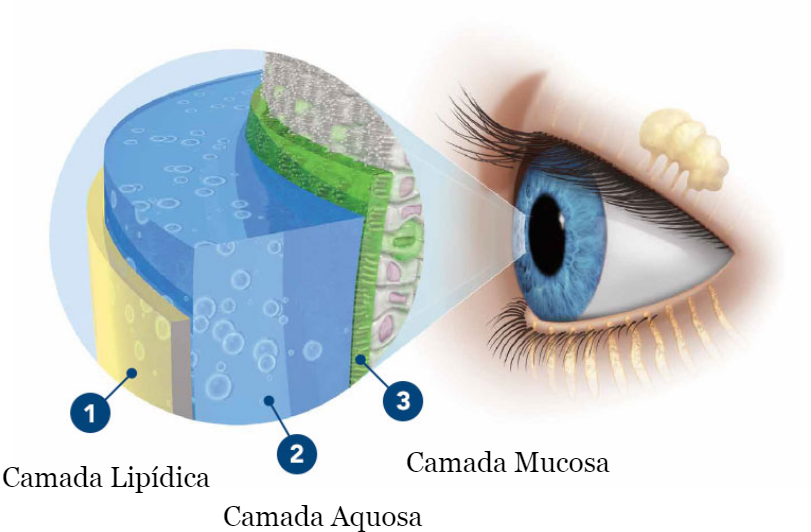
\includegraphics[width=0.6\textwidth]{figs/ImagemCamadas.png}
    \legend{Fonte: Adaptado de \cite{UnderstandingDryEye}.}
    \label{fig:EstruturaFilmeLacrimal}
\end{figure}

A Síndrome do Olho Seco evaporativo é causada pela deficiência da camada lipídica. Assim, a avaliação dessa camada é uma das formas utilizadas para avaliar o filme lacrimal \cite{korb2002tear}.

\subsection{Imagens e Síndrome do Olho Seco}
\label{sec:imgPatologia}

A Síndrome do Olho Seco é uma doença multifatorial da superfície ocular que resulta em desconforto, distúrbios visuais e instabilidade do filme lacrimal. Embora haja portadores assintomáticos, a maioria tem como principais sintomas: sensação de corpo estranho, queimação, instabilidade do filme lacrimal com potencial dano à superfície ocular, prurido, fotofobia, embaçamento visual e lacrimejamento excessivo, o que pode causar impacto na qualidade de vida. Este distúrbio é mais comum em adultos com mais de 40 anos e afeta principalmente as mulheres \cite{valim2015current}.

Existem duas categorias da Síndrome do Olho Seco, de acordo com a classificação do DEWS (\textit{International Workshop on Dry Eye} - Workshop Internacional sobre Olho Seco): deficiência aquosa e aumento da evaporação. A principal causa da Síndrome do Olho Seco do tipo de deficiência aquosa é a síndrome de Sjögren (SS). Além da SS, outras doenças causam a diminuição da produção das lágrimas como: lúpus eritematoso sistêmico, reumatoide, esclerose sistêmica, sarcoidose, artrite, linfoma, diabetes, episclerite, HIV ou infecções por vírus da hepatite C, deficiência da glândula lacrimal, obstrução do ducto lacrimal, hipossecreção reflexa e uso de medicações sistêmicas \cite{dry2007definition, lemp2012distribution, sivaraj2007ocular, waszczykowska2013prevalence, fox1994systemic}.

A Síndrome do Olho Seco evaporativo pode ser causado por várias outras doenças, como blefarite, psoríase, rosácea, dermatite seborreica, conjuntivite alérgica e distúrbios palpebrais (paralisia do nervo facial, doença de Graves), uso prolongado de lentes de contato e medicamentos de uso tópico e uso sistêmico. Entretanto, estudos mostram que ambos os tipos geralmente coexistem, e a forma isolada evaporativa é mais comum que a deficiência isolada aquosa \cite{dry2007definition, lemp2012distribution, fonseca2010olho}.

O diagnóstico da patologia é uma tarefa difícil devido à sua etiologia multifatorial e vários testes clínicos, que podem ser utilizados tanto para o diagnóstico quanto para o tratamento. A avaliação dos padrões de interferência que categorizam a camada lipídica através da classificação do filme lacrimal é um dos testes mais comuns para diagnosticar a Síndrome do Olho Seco \cite{GUILLON1998S31}. Essa avaliação pode ser realizada utilizando diferentes tipos de instrumentos: Tearscope Plus, Interferômetro Doane, Tomografia de Coerência Óptica (OCT), etc.

%A espessura e a regularidade da camada lipídica são categorizadas observando a aparência e a cor do padrão de interferência entre a camada lipídica e as camadas subjacentes.O instrumento usado em conjunto com um biomicroscópio não iluminado fornece ampliação adequada da imagem.

O Interferômetro Doane apresentado e desenvolvido por Doane \cite{doane1989instrument}, consiste originalmente em uma fonte de luz e um sistema de observação que captura a aparência do filme lacrimal usando um sistema baseado em vídeo. Este modelo permite que as mudanças dinâmicas que ocorrem ao longo do tempo sejam gravadas, permitindo que clínicos avaliem rapidamente a espessura da camada lipídica.

\citeonline{thai2004effect} utilizaram o Interferômetro para medir a taxa de evaporação, características de desgaste e mudanças na camada lipídica do filme lacrimal. Para isto, eles propuseram um sistema para classificação do filme lacrimal em imagens de diferentes categorias. Com base em tal estudo, uma nova escala de classificação composta por cinco categorias foi proposta em \cite{remeseiro2015automatic} uma vez que o uso de uma câmera digital produziu mudanças nos detalhes vistos nas imagens digitais. Essas categorias são: detritos, franjas finas, coalescente de franjas finas, franjas fortes e coalescente de franjas fortes.

O Tearscope Plus é o instrumento projetado por Guillon para avaliação rápida da espessura da camada lipídica \cite{GUILLON1998S31}. Ele projeta uma fonte cilíndrica de luz fluorescente branca fria sobre a camada lipídica e, portanto, qualquer fenômeno observado é exclusivo de sua fonte de luz específica. Em geral, as imagens do Tearscope são analisadas durante a realização do exame, sem qualquer processo de aquisição. No entanto, existem alguns estudos que utilizaram procedimentos de aquisição de vídeo/imagens \cite{efron2012}, \cite{king1999three}, que auxiliam o observador a classificar corretamente os padrões e são indispensáveis para a análise computacional.

Os conjuntos de imagens capturadas pelo Tearscope Plus podem conter cinco categorias: malhas abertas, malhas fechadas, ondas, amorfa e de franja. Em ambos instrumentos, a variabilidade da aparência dos padrões de interferência da camada lipídica resultam em grandes variações inter e intra observadoras. Portanto, a classificação visual dos padrões é uma tarefa clínica difícil, especialmente com camadas lipídicas mais finas que não possuem características de cor e/ou morfológicas \cite{garcia2013new}.

Nas próximas seções desse capítulo são apresentados os conceitos teóricos utilizados pelo método proposto para a classificação automatizada da camada lipídica em imagens do filme lacrimal. Os aspectos fisiológicos dos olhos expostos nessa seção serão levados em consideração para o aperfeiçoamento das técnicas propostas no método apresentado no próximo capítulo.

\section{Processamento Digital de Imagens}
\label{sec:PDI}

Em geral, o processamento digital de imagens é definido como um conjunto de técnicas computacionais que transformam uma imagem de entrada em uma saída desejada \cite{gonzalez2010processamento}. Esse conjunto de técnicas possibilita extrair e identificar informações das imagens e melhorar a qualidade visual de aspectos estruturais, facilitando a percepção humana e a interpretação automática por meio de máquinas \cite{pedrini2008analise}.

O principal objetivo do processamento de imagens é auxiliar a compreensão do mesmo, entretanto, existem vários algoritmos com finalidades muito específicas, que juntos formam a metodologia final. Portanto, uma metodologia difere de outra na maneira que compõe seus passos ou ferramentas, mas tipicamente obedecem as etapas apresentadas por Gonzalez e Woods (2010)\nocite{gonzalez2010processamento}, conforme apresentado na~\autoref{fig:passosProcessamentoImagens}.

As etapas fundamentais para resolução do problema, são\cite{gonzalez2010processamento}: aquisição das imagens digitais, pré-processamento, segmentação, representação, descrição e, reconhecimento e interpretação. O resultado gerado por uma etapa é utilizado como entrada na etapa seguinte onde cada entrada e resultado pode ou não ser uma imagem digital. Uma metodologia de processamento de imagens pode conter apenas um subconjunto de todas as etapas apresentadas \cite{BRAZ:2014}.

\begin{figure}[ht!]    
	\centering
	\caption{Etapas fundamentais em processamento digital de imagens.}
	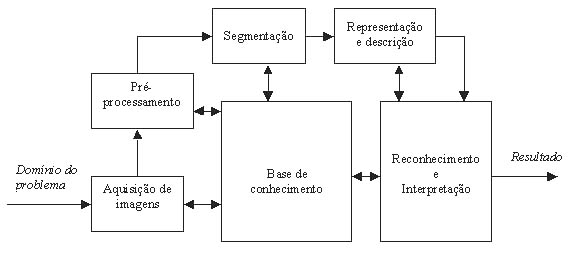
\includegraphics[width=0.90\textwidth]{figs/passosProcessamentoImagens.png}
	\legend{Fonte: Adaptado de \cite{gonzalez2010processamento}.}
	\label{fig:passosProcessamentoImagens}
\end{figure}

As etapas necessárias após a definição e delimitação do problema, foram: segmentação, extração de características, seleção de características e reconhecimento de padrões, com base no modelo apresentado. Portanto, no restante deste capítulo são abordados os aspectos teóricos das técnicas utilizadas no método proposto desta dissertação.

\begin{comment}
\section{Pré-processamento}
\label{sec:preprocessamento}

Nesta seção são apresentadas as técnicas de melhoramento de imagens utilizadas no método proposto, visando aprimorar o desempenho da segmentação, extração de características e reconhecimento de padrões. Para o desenvolvimento do método foram utilizadas técnicas de realce para o tratamento do contraste das imagens e quantização para a digitalização dos valores de amplitude.  

%que utiliza o valor máximo e mínimo da imagem digitalizada e divide a escala de cinza em intervalos iguais de acordo com o número de \textit{bits} definidos. Uma forma de calcular 

\subsection{Filtro Homomórfico}

O filtro homomórfico é usualmente utilizado em melhoramento de imagens digitais. Essa técnica analisa separadamente as informações de reflectância e iluminação, obtendo uma imagem com realce das altas frequência (reflectância) e atenuação das baixas frequências (iluminação). A iluminância $i(x,y)$ representa a quantidade de luz que incide sobre o \textit{pixel}. Já a reflectância $r(x,y)$ indica quanto dessa luz incidente é refletida. A ideia central é que a iluminação varie pouco ao longo da imagem em relação à reflectância.

De acordo com Melo et al. (2005)\nocite{de2005system}, a o filtro homomórfico tem como entrada a função $f(x,y)$, que representa a imagem de entrada em níveis de cinza. Em seguida, os valores dos \textit{pixels} são convertidos para o logaritmo natural (\autoref{eq:logaritmo}), onde ocorre a separação dos componentes de iluminação e reflectância. Na imagem logarítmica é aplicado o filtro passa-baixa\footnote{permite a passagem dos componentes de mais baixa frequência, atenuando o contraste.} e o filtro passa-alta\footnote{permite a passagem dos componentes de alta frequência com facilidade, porém reduz a amplitude das frequências abaixo da frequência de corte.} resultando em $log(i(x,y))$ e $log(r(x,y))$, respectivamente.

\begin{equation}
\label{eq:logaritmo}
f(x, y) = log(1 + f(x, y))
\end{equation}

As imagens resultantes dos filtros passa-baixa e passa-alta são multiplicadas por valores $\alpha$ e $\beta$, onde $\alpha$ < 1 e $\beta$ > 1, respectivamente. Dessa forma, diminuirá os limites amplos de intensidade em $log(i(x,y))$ e aumentará o contraste local em $log(r(x,y))$. Posteriormente, $\alpha \times log(i(x,y))$ e $\beta \times log(r(x,y))$ são somadas e normalizadas entre faixa de valores 0 e 1. Finalmente, é calculado o exponencial da imagem normalizada (evita tender ao infinito), seguida da normalização para os níveis de cinza (0 - 255) e aplicação da equalização do histograma. Na~\autoref{fig:filtroH2} é apresentado o esquema de aplicação do filtro homomórfico.

\begin{figure}[ht!]
    \centering
    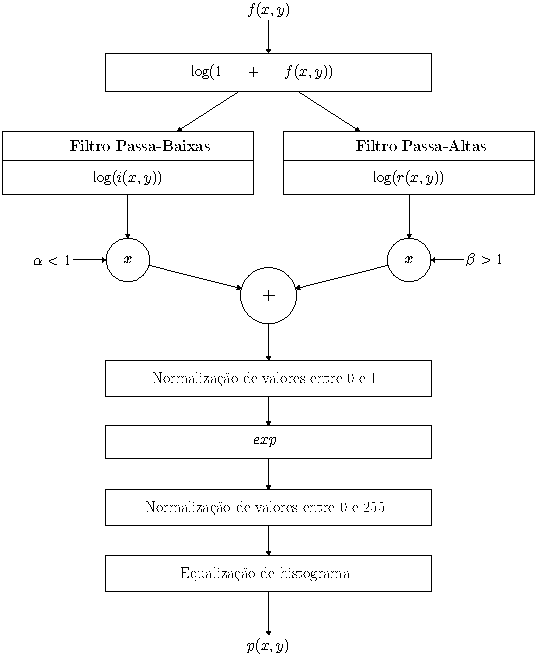
\includegraphics[width=12cm]{figs/fig_homomorphicFilter.pdf}
    \caption{Esquema de aplicação do filtro homomórfico. Fonte: \cite{gomes:2017}.}
    \label{fig:filtroH2}
\end{figure}

Nesta dissertação, o filtro homomórfico foi utilizado para corrigir a iluminação não uniforme, minimizando a influência da iluminação no processamento de imagens. A~\autoref{fig:filtroH} (b) apresenta o resultado obtido com a aplicação do filtro homomórfico a partir de uma imagem de entrada da base VOPTICAL\_LS (\autoref{fig:filtroH}).

\begin{figure}[ht!]
    \centering
    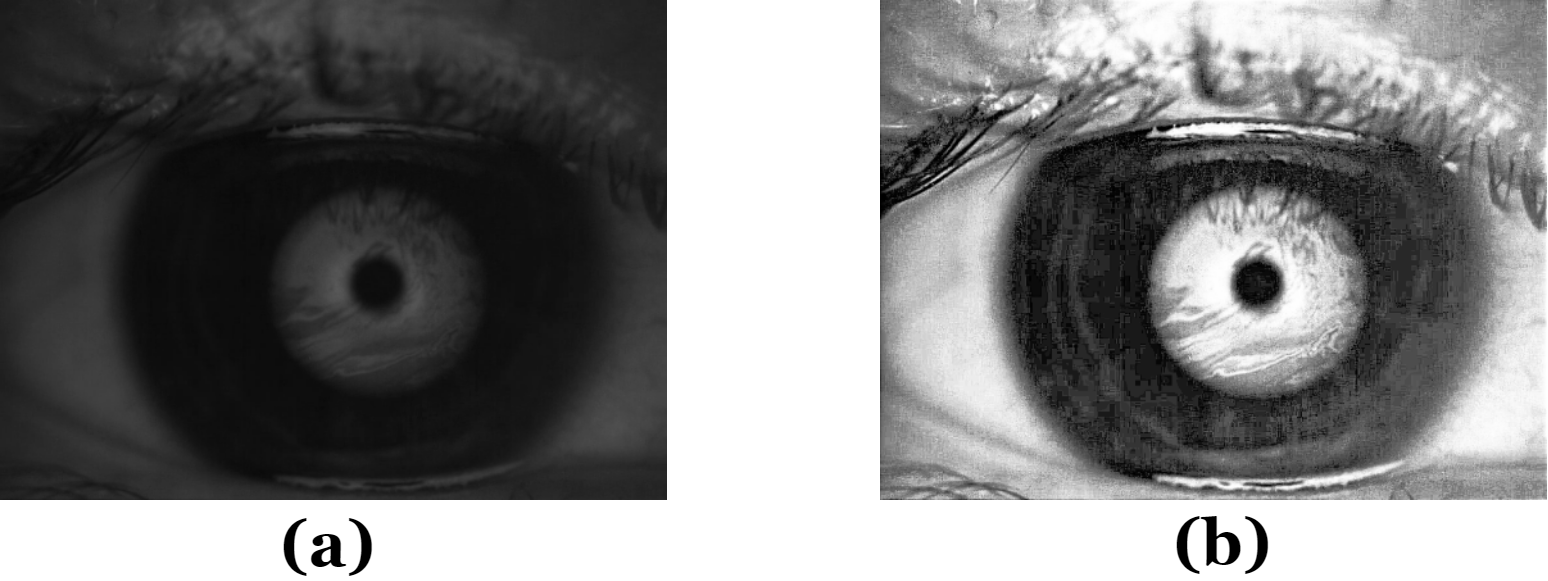
\includegraphics[width=11cm]{figs/FiltroH.png}
    \caption{Exemplo de utilização do filtro homomórfico (a) imagem original; (b) imagem após aplicação do filtro homomórfico.}
    \label{fig:filtroH}
\end{figure}
\end{comment}

\section{Extração de Características}
\label{sec:extCaracteristicas}

A extração de características tem o objetivo de extrair informações quantitativas de interesse ou que sejam básicas para discriminação entre as classes de objetos. Portanto, esta etapa visa obter medidas descritivas das bases de imagens, as quais formarão os vetores de características que serão usados nas etapas de seleção e classificação. A etapa de extração de características pode ser dividida em duas categorias de análise, sendo elas: textura e forma.

Em uma análise por textura, o objetivo é descrever aspectos da imagem no que diz respeito a suavidade, rugosidade e regularidade \cite{gonzalez2008digital}, possibilitando distinguir regiões da imagem que apresentam as mesmas características de padrões \cite{azevedo2003computaccao}. Já em uma análise baseada na forma, o intuito é extrair informações que mensuram sobre propriedades morfológicas da imagem, caracterizando a forma e aparência dos objetos
através do contorno ou da área do objeto em estudo \cite{BRAZ:2014}.

O procedimento de extração de características adotado nesta dissertação é distribuído em análise de texturas baseadas em geoestatística \cite{BRAZJUNIOR20091063} e outra em índices de diversidade \cite{16085910409503825}. Para tal, as seções seguintes apresentam as fundamentações dos descritores propostos para o tipo de análise por textura.

\section{Análise por Textura}

A análise de textura é, em princípio, uma técnica para avaliar a posição e a intensidade das características do sinal, ou seja, \textit{pixels} e sua intensidade em imagens digitais. As características de textura são, na verdade, parâmetros matemáticos calculados a partir da distribuição de \textit{pixels}, que caracterizam o tipo de textura e, portanto, a estrutura subjacente dos objetos mostrados na imagem \cite{CASTELLANO20041061}. De acordo com os métodos empregados para avaliar as inter-relações dos \textit{pixels}, três formas de análise de textura são usadas em processamento de imagem, categorizadas como: métodos estatísticos, estruturais e baseados em modelos \cite{gonzalez2010processamento}.

A abordagem estatística define a textura como um conjunto de medidas locais extraídas do padrão, descrevendo as imagens através de regras estatísticas que administram tanto a distribuição quanto a relação entre os diferentes níveis de cinza. A abordagem estrutural considera a textura como um conjunto de sub-padrões espaciais na imagem com arranjos espaciais repetitivos regulares, conforme regras bem definidas \cite{morais1999discriminaccao}. Finalmente, na abordagem baseada em modelos a textura pode ser considerada como uma realização de um processo estocástico dirigido por parâmetros, que são utilizados como características \cite{felipe2002utilizando}.

Nesta dissertação, foram utilizados para caracterizar a textura das imagens do filme lacrimal, a função K de \textit{Ripley} e os índices de diversidade filogenética, que são medidas estatísticas.

\subsection{Função K de \textit{Ripley}}
\label{sec:kripley}

A função K de \textit{Ripley} é comumente usada em análise de dados espaciais, sendo frequentemente empregada na ecologia, para descrever a distribuição espacial de árvores e outras espécies em uma floresta. Nos últimos trinta anos, sua aplicação também foi utilizada nas mais diversas áreas como: epidemiologia, geomorfologia, criminologia, geologia, etc \cite{lancaster2004spatial}.

Essa técnica pode ser usada para resumir um padrão de pontos, testar hipóteses sobre o padrão, estimar parâmetros e ajustar modelos~\cite{ripley1977modelling}. A função é definida na Equação~\ref{equacao:equacaoRipley}:

\begin{equation}
\label{equacao:equacaoRipley}
R(d,i) = \sqrt{\frac{Ak(i,j)}{N}}, i \neq j,
\end{equation}onde $d$ representa a função de distância usada na análise, $A$ indica a área da região em questão, calculada a partir do ponto de referência $i$ sob a distância $d$. $N$ o total de pontos da amostra, e $k$ é a função de pertinência que verifica se $j$ está contido no conjunto de análise determinado por $i$ e $d$. Ou seja, cada padrão espacial pontual é examinado separadamente dos demais, e tratado como a ocorrência ou não de uma mesma intensidade dentro da distância especificada.

Em suma, a função K de \textit{Ripley} calcula uma relação do total de indivíduos de uma determinada espécie distribuída em uma região de estudo. Segundo \cite{martins2007detecccao}, além do uso convencional (círculos) da função K de \textit{Ripley}, foi proposta também uma nova forma de aplicação da função, através da análise dos padrões de pontos em anéis. Basicamente, a modificação consiste em substituir a região de interesse dada pela \autoref{fig:ripleyCircAneis} (a) pela região compreendida entre dois círculos concêntricos, como na \autoref{fig:ripleyCircAneis} (b). Além dessas duas abordagens, formas complexas como, janelas e diagonais também podem ser aplicadas.

\begin{figure}[ht]
    \centering
    \caption{Abordagens da função K de \textit{Ripley}. (a) círculos; (b) anéis.}
     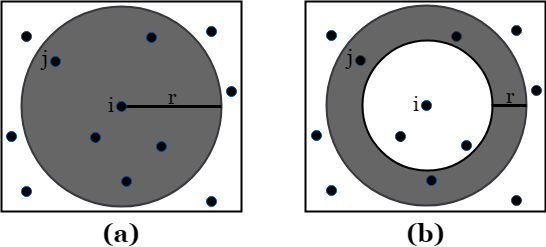
\includegraphics[width=8cm]{figs/RipleyCircAneis1.png}
     \legend{Fonte: Adaptado de \cite{martins2007detecccao}.}
    \label{fig:ripleyCircAneis}
\end{figure}

O cálculo do raio de cada círculo é baseado no raio máximo determinado pela região. Inicialmente, é necessário calcular a menor dimensão da Região de Interesse (ROI). Assim, o raio máximo é representado pela metade do valor da menor dimensão. A partir do raio máximo, calculam-se os demais através da alteração de proporção em relação ao primeiro, dada pela \autoref{equacao:equacaoCirc}.

%Para cada círculo, o cálculo dos raios é baseado no seu raio máximo. Inicialmente, é necessário calcular o menor tamanho da Região de Interesse (ROI). O raio máximo é metade do menor tamanho de ROI. Então, os outros raios podem ser calculados usando diferentes proporções do raio máximo (\autoref{equacao:equacaoCirc}).

\begin{equation}
\label{equacao:equacaoCirc}
Raio_{i} = \frac{Raio_{max}}{i},
\end{equation}
onde $i$ = $1,2,3...,n$, e $n$ é a quantidade de raios determinados pela aplicação.

Para calcular a divisão em anéis, segue-se o mesmo princípio do cálculo da divisão em círculos. A diferença está no fato de anéis não possuírem áreas comuns entre si, como tem os círculos concêntricos. Assim, o raio máximo do anel interno é utilizado como um raio mínimo para o próximo.

A partir do mesmo cálculo do raio máximo obtido pela divisão de círculos, os raios mínimos e máximos dos anéis são obtidos usando as Equações \ref{equacao:equacaoMin} e \ref{equacao:equacaoAnelMax}, respectivamente.

\begin{equation}
\label{equacao:equacaoMin}
Raio_{min} (i) = \frac{Raio_{max}}{n}i
\end{equation}
e
\begin{equation}
\label{equacao:equacaoAnelMax}
Raio_{max} (i) = \frac{Raio_{max}}{n}(i + 1),  
\end{equation}onde $i$ = $1,2,3...,n$, e $n$ é a quantidade de raios determinados pela aplicação.

Portanto, as divisões criam novas representações de regiões circulares e concêntricas da região, a partir das ROIs das imagens. Assim, cada divisão gera recortes individualizados que passarão por todo o processo de extração de características.

\subsection{Índices de Diversidade e Diversidade Filogenética}
\label{sec:indicesDiversidade}

A diversidade é um termo comumente empregado na Ecologia para medir a biodiversidade de um ecossistema, com intuito de identificar a distribuição de um grupo de espécies e as suas relações. De modo geral, o objetivo de um índice de diversidade é descrever a variedade de espécies presentes em uma comunidade ou determinada região, que tais representam um conjunto de espécies que ocorrem em um determinado lugar e tempo \cite{magurran2013measuring}.

O uso dos índices de diversidade são comuns na literatura para extrair características em nódulos pulmonares \cite{de2017computer,de2017lung,de2018classification} e na diferenciação de massas benignas e malignas em mamografias \cite{CARVALHO2018210, de2015classification}. Diferentemente dessas aplicações, os índices de diversidade filogenética foram utilizados no método proposto para extrair características em imagens do filme lacrimal para classificar as categorias da camada lipídica. Para tanto, foram utilizados três grupos dos índices: (1) baseados na distância entre pares de espécies; (2) baseados na topologia; e (3) baseados em caminho mínimo.

\begin{comment}
%Os índices do primeiro grupo são capazes de mensurar a cerca das relações de parentesco que determinadas espécies possuem, como por exemplo, a quantidade de ancestrais comuns que existem entre determinadas espécies. O segundo grupo, explora o grau de parentesco entre as espécies relacionando possíveis ancestrais em comum. Já o terceiro, possuem a propriedade de aferir o quão distante estão as espécies presentes na comunidade, considerando a distância filogenética, calculada a partir de uma árvore filogenética, podendo ser representada em forma de dendrograma, como apresentada na Figura~\ref{fig:Cladograma}.

%foi um dos primeiros a propor o uso de métodos baseados em topologia, refletindo a ordem de ramificação filogenética dentro de um grupo. Nesta abordagem, cada tipo de comunidade é ponderada pelo número de nós entre as espécies e a raiz da árvore filogenética (dendrograma); Desta forma, as espécies com os maiores pesos são aquelas com maior distância da raiz. Em nosso trabalho, as distâncias são representadas pelo número de nós entre as espécies.

%determinam além das propriedades filogenéticas a topologia pela qual as espécies se distribuem no dendrograma

%denotam relações evolutivas.

%Nesta árvore, os nós das folhas representam as espécies analisadas, os nós internos correspondem a algum antepassado comum e as arestas indicam a distância filogenética entre duas espécies. Assim, é possível fazer uma conexão evolutiva entre as espécies \cite{carvalho2016metodos}.

%Para implementar essa ideia, a primeira etapa é realizar uma correspondência entre os termos usados na biologia e os utilizados neste trabalho. A Tabela~\ref{table:descricao} apresenta essa correspondência.

%os ancestrais são representados pelos nós internos no cladograma
%A escolha dos índices de diversidade filogenética foi devido ao seu grande potencial na caracterização de texturas em imagens.
\end{comment}

Os índices do primeiro grupo são capazes de mensurar acerca das relações de parentesco que determinadas espécies possuem, como por exemplo, a quantidade de ancestrais comuns que existem entre determinadas espécies. O segundo grupo, reflete a ordem de ramificação filogenética dentro de um grupo. Já o terceiro, possui a propriedade de aferir o quão distante estão as espécies presentes na comunidade, considerando a distância filogenética, calculada a partir de uma árvore filogenética \cite{carvalho2016metodos}.

%que é uma representação gráfica usada para descrever a relação filogenética entre espécies ancestrais

%Árvores filogenéticas são usadas na biologia para descrever as relações evolutivas entre as espécies, a fim de determinar possíveis ancestrais comuns. As árvores filogenéticas podem ser representadas em forma de cladograma inclinado para descrever a relação filogenética entre espécies ancestrais \cite{baxevanis2004bioinformatics}. A Figura~\ref{fig:Cladograma} ilustra uma árvore filogenética dos macacos em forma de cladograma. Note que um chimpanzé tem maior proximidade filogenética com humanos do que um siamango. Nesta árvore, os nós da folha são as espécies analisadas, os nós internos correspondem a algum ancestral comum, e as arestas indicam a distância filogenética entre duas espécies \cite{carvalho2016metodos, baxevanis2004bioinformatics}.

Árvores filogenéticas e filogenia são usadas na biologia para descrever as relações evolutivas entre as espécies, a fim de determinar possíveis ancestrais comuns \cite{baxevanis2004bioinformatics}. A Figura~\ref{fig:Cladograma} ilustra uma árvore filogenética dos macacos em forma de cladograma inclinado. Note que um chimpanzé tem maior proximidade filogenética com humanos do que um siamango. Nesta árvore, os nós da folha são as espécies analisadas, os nós internos correspondem a algum ancestral comum, e as arestas indicam a distância filogenética entre duas espécies \cite{carvalho2016metodos, baxevanis2004bioinformatics}.

%Árvores filogenéticas são usadas na biologia para descrever as relações evolutivas entre as espécies, a fim de determinar possíveis ancestrais comuns. As árvores filogenéticas podem ser representadas em forma de cladograma inclinado \cite{baxevanis2004bioinformatics} como apresentado na Figura~\ref{fig:Cladograma}, que ilustra uma árvore filogenética dos macacos. Note que um chimpanzé tem maior proximidade filogenética com humanos do que um siamango. Nesta árvore, os nós da folha são as espécies analisadas, os nós internos correspondem a algum ancestral comum, e as arestas indicam a distância filogenética entre duas espécies \cite{carvalho2016metodos, baxevanis2004bioinformatics}.

\begin{figure}[ht!]
    \centering
    \caption{Árvore filogenética representada como cladograma.}
     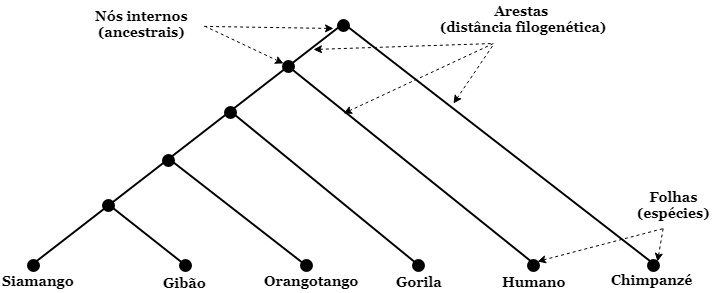
\includegraphics[width=12cm]{figs/Cladograma2.png}
     \legend{Fonte: Adaptado de \cite{baxevanis2004bioinformatics}.}
    \label{fig:Cladograma}
\end{figure}
%\FloatBarrier

Árvores filogenéticas combinadas com índices de diversidade filogenética comparam padrões de comportamento entre espécies de diferentes áreas e, descrevem suas relações evolutivas entre seus antepassados \cite{vane1991protect}. Para implementar essa ideia, o primeiro passo é fazer uma correspondência entre os termos usados na biologia e os utilizados neste trabalho (Tabela~\ref{table:descricao}).

A~\autoref{table:descricao} apresenta a correspondência dentro do contexto de processamento de imagens. A comunidade é representada pela ROI, seus indivíduos são representados pelos \textit{pixels}, os níveis de cinza são suas espécies e a distância filogenética é representada pelo número de arestas entre duas espécies.

\definecolor{lightgray}{gray}{0.94}
\begin{table}[!ht]
\centering
\onehalfspacing
\rowcolors{1}{}{lightgray}
\caption{Correspondência entre os termos da biologia e o método proposto.}
\label{table:descricao}
\begin{tabular}{lp{7cm}l}
\hline
\multicolumn{1}{c}{\textbf{Biologia}} & \multicolumn{1}{c}{\textbf{Método Proposto}}          \\ \hline \hline
Comunidade                            & Região de interesse da imagem do filme lacrimal      \\
Espécies                              & Número máximo de valores de níveis de cinza na região \\
Indivíduos                             & Quantidade de \textit{pixels} de uma determinada espécie \\
%Ancestrais                            & Número de nós internos no dendrograma                 \\
Distância filogenética                & Número de arestas entre duas espécies                 \\ \hline
\end{tabular}
\end{table}
\FloatBarrier

A Figura~\ref{fig:ExemploCladograma} mostra um exemplo da construção de um árvore filogenética em forma de cladograma a partir de uma amostra de imagem original. Esta imagem contém três níveis de cinza, que são preto (P), cinza (C) e branco (B), bem como as espécies que compõem a comunidade. O número de \textit{pixels} para P é 4, C é 2 e B é 3, compreendendo assim os indivíduos da comunidade. A representação genérica da árvore e sua matriz de distância para a imagem da Figura~\ref{fig:ExemploCladograma} (a) são mostradas na Figura~\ref{fig:ExemploCladograma} (b) e (c), respectivamente.

\begin{figure}[ht!]
    \centering
    \caption{Imagem sintética para exemplificar o cladograma. (a) amostra de uma imagem original; (b) árvore enraizada na forma de cladograma inclinado e (c) matriz de distâncias.}
     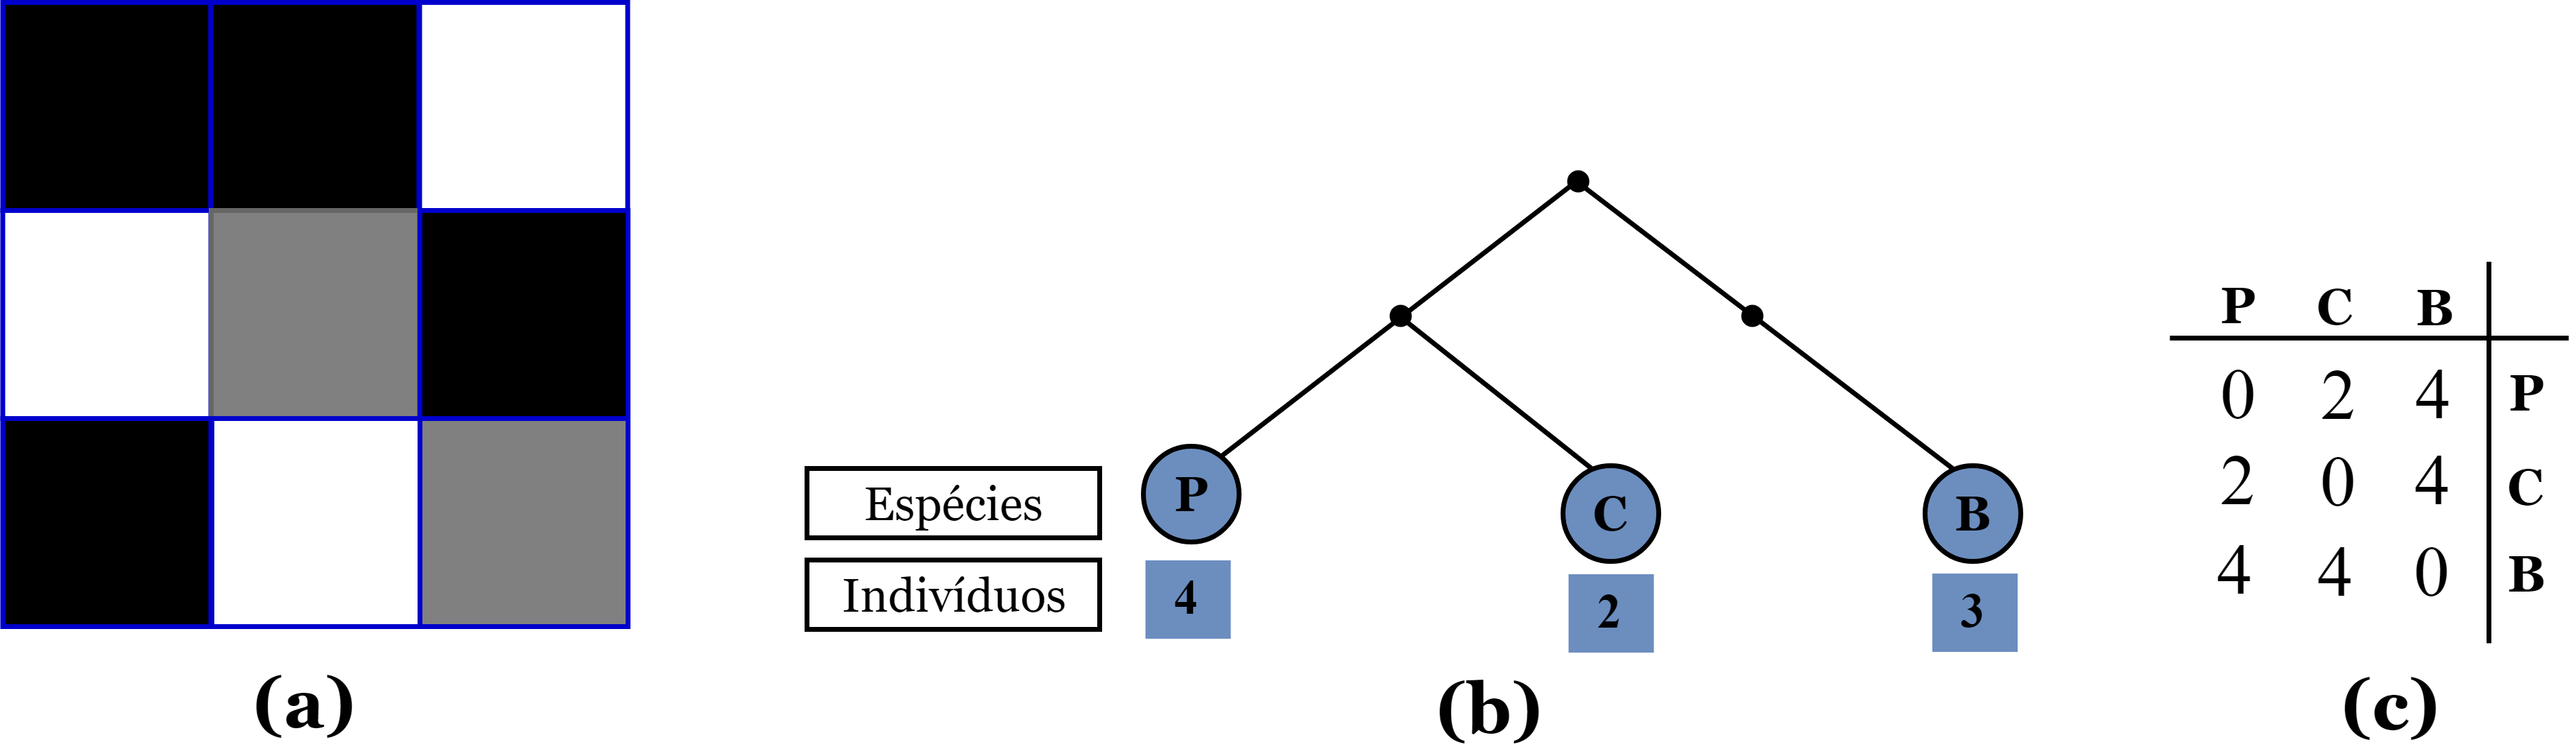
\includegraphics[width=16cm]{figs/ExemploCladogramaFinal.png}
     \legend{Fonte: Adaptado de \cite{CARVALHO2018210}.}
    \label{fig:ExemploCladograma}
\end{figure}
\FloatBarrier

A informação requerida de um determinado cladograma para o cálculo da diversidade filogenética pode ser resumida por uma matriz de distâncias entre espécies, obtida a partir do cladograma. Os valores dentro da matriz de distância são interpretados como a distinção entre cada par de espécies ou entre uma espécie específica e todas as outras \cite{CARVALHO2018210}. Assim, os detalhes fundamentais de cada grupo de índices são coletados para composição dos descritores propostos. Nas próximas seções serão apresentados maiores detalhes de cada grupo, e como é realizado o cálculo de cada um dos índices.

%já que estes índices se complementam, isto é, um grupo é capaz de mensurar alguma riqueza de propriedade que outro grupo não consegue.

\subsubsection{Índices de Diversidade Filogenética Baseados na Distância entre Pares de Espécies}
\label{sec:indicesPE}

Os índices que medem as relações de distância entre pares de espécies são baseados na matriz de distância de todas as espécies da comunidade. Estes índices podem ser interpretados como a distinção entre cada par de espécies ou de cada espécie em particular para todas as outras. Nessa abordagem, as distâncias são representadas pelo número de arestas entre as espécies, calculadas sobre a árvore mapeada (\autoref{fig:Cladograma}). Nesse grupo, cinco índices são utilizados: a entropia quadrática intensiva \cite{izsak2000link}, a entropia quadrática extensiva \cite{izsak2000link}, a distinção taxonômica média \cite{pienkowski1998taxonomic}, a distinção taxonômica total \cite{krwarwick} e a medida de diversidade pura \cite{gerlinger2012intratumor}.

A entropia quadrática intensiva ($I$) estabelece uma ligação entre os índices de biodiversidade e índices de diversidade \cite{izsak2000link}. O índice $I$ representa o número de espécies e as relações taxonômicas, quando existem os mesmos valores formais ou hipotéticos em abundância. Portanto, $I$ expressa a distância taxonômica média entre duas espécies. As relações entre espécies influenciam o valor de $I$, diferentemente de outros índices de diversidade \cite{izsak2000link}. O índice $I$ é dado pela~\autoref{equacao:equacaoI}.
\begin{equation}
\label{equacao:equacaoI}
I = \left [ \sum d_{i,j} \right ] / s^{2},
%I = [\frac{\sum\limits_{i=1}^{i=n-1}\sum\limits_{j=1}^{j=n-1} d_{i,j}}{s^{2}}]
\end{equation}
onde a distância entre as espécies $i$ e $j$ é representada por $d_{i,j}$ e $s$ o número de espécies.

Em relação às propriedades do índice, a monotonicidade é geralmente necessária para métricas de diversidade. Para uma determinada medida $J$, essa propriedade significa que: $J (A \cup \left \{ x \right \}) > J(A)$, garante que o valor do índice aumentará adicionando uma nova espécie $x$ a um conjunto de espécies $A$. Portanto, $I$ não é um índice de diversidade ideal, uma vez que não satisfaz esse requisito. Para resolver este problema, a entropia quadrática extensiva ($E$) \cite{izsak2000link} foi proposta com base em $I$. $E$ representa a soma das diferenças de espécies. O índice $E$ tem a propriedade de monotonicidade, já que para qualquer conjunto de espécies $A$, se uma nova espécie $x$ for adicionada, o valor de $E$ será modificado. O índice $E$ é calculado na Equação~\ref{equacao:equacaoE}.
\begin{equation}
\label{equacao:equacaoE}
E = \sum d_{i,j},
%E = \sum\limits_{i=1}^{i=n-1}\sum\limits_{j=1}^{j=n-1} d_{i,j}
\end{equation}
onde a distância entre as espécies $i$ e $j$ é representada por $d_{i,j}$.

A distinção taxonômica média ($DTM$) e a distinção taxonômica total ($DTT$) foram originalmente desenvolvidas com base nas relações taxonômicas. No entanto, podem ser facilmente adaptadas às informações filogenéticas \cite{schweiger2008comparative}. A $DTM$ refere-se à distância taxonômica média entre duas espécies \cite{pienkowski1998taxonomic} e $DTT$ representa a distinção taxonômica média de todas as espécies dentro da comunidade. $DTM$ e $DTT$ são, respectivamente, definidos nas Equações~\ref{equacao:equacaoIDTM} e \ref{equacao:equacaoIDTT}.
\begin{equation}
\label{equacao:equacaoIDTM}
DTM = \left [ \sum \sum_{i<j}d_{i,j} \right ] / \left [ s(s - 1)/2 \right ]
%DTM = [\frac{\sum\limits_{i=1}^{i=n-1}\sum\limits_{j=1}^{j=n-1}d_{i,j}}{\frac{s(s-1)}{2}}]
\end{equation}
e
\begin{equation}
\label{equacao:equacaoIDTT}
DTT = \sum_{i}\left [ \left ( \sum_{i \neq j}d_{i,j} \right )\left (s - 1  \right ) \right ],
%DTT = [\frac{\sum\limits_{i=1}^{i=n-1}\sum\limits_{j=1}^{j=n-1}d_{i,j}}{(s-1)}]
\end{equation}
onde $d_{i,j}$ representa a distância entre as espécies $i$ e $j$, e o número de espécies é definido por $s$.

Finalmente, o índice de diversidade pura ($IDP$) verifica a distância de uma espécie para seu vizinho mais próximo \cite{faith1992conservation}. $IDP$ é definido na Equação~\ref{equacao:equacaoIDP}.
\begin{equation}
\label{equacao:equacaoIDP}
IDP = \sum d_{i} _{ } _{ }_{min},
%IDP =\sum\limits_{i=1}^{i=n-1}\textit{$d_{i}$} \textit{$_{min}$}
\end{equation}
onde $d_{i} _{ } _{ }_{min}$ representa a menor distância do vizinho mais próximo da espécie $i$ em relação as todas as outras espécies.

\subsubsection{Índices de Diversidade Filogenética Baseados na Topologia}
\label{sec:indicesT}

Os índices de diversidade filogenética baseados na topologia refletem a ordem de ramificação filogenética dentro de um grupo. Nesta abordagem, cada espécie de uma comunidade é ponderada de acordo com o número de nós entre as espécies e a raiz da árvore filogenética. Portanto, espécies com pesos maiores são aquelas com maiores distâncias da raiz no cladograma \cite{vane1991protect}. Esse grupo é composto por dois índices: a soma básica dos pesos e soma dos pesos normalizados \cite{keith2005taxonomic,posadas2001using,vane1991protect}, que estão relacionados às espécies da comunidade que indicam o grau de similaridade entre elas.

A soma básica de pesos ($Q$) é o quociente de todos os nós dividido pelo número de nós entre a raiz e uma espécie, que representa a soma das contribuições de cada espécie para a diversidade. O índice $Q$ é definido na Equação~\ref{equacao:equacaoQ1}.
\begin{eqnarray}
\label{equacao:equacaoQ1}
Q = \sum Q_{i} \nonumber \\
Q_{i} = I/I_{i} \\
I = \sum I_{i}, \nonumber, 
\end{eqnarray}
onde $ Q_{i}$ é o quociente do total de nós raiz para todas as espécies por $ I_{i}$, que é o número de nós entre a raiz e a espécie $i$.

A soma dos pesos normalizados ($W$) representa para cada espécie o peso normalizado, isto é, os valores de $Q$ de cada espécie dividido pelo valor de $Q_{min}$. $W$ é calculado pela Equação~\ref{equacao:equacaoW2}.
\begin{eqnarray}
\label{equacao:equacaoW2}
W = \sum W_{i} \nonumber \\
W_{i} = Q_{i}/Q_{min},
\end{eqnarray}
onde $Q_{min}$ representa o quociente do caminho mínimo da raiz para a espécie.

%índices de diversidade filogenética baseados em topologia, que determinam além das propriedades filogenéticas a topologia pela qual as espécies se distribuem no dendrograma. Em outras palavras, através desses índices, é possível explorar o grau de parentesco entre as espécies relacionando possíveis ancestrais em comum. Portanto, viabilizando a caracterização da relação homogeneidade e heterogeneidade com base na topologia das espécies. %%% ja estava comentado

\subsubsection{Índices de Diversidade Filogenética Baseados em Caminho Mínimo}
\label{sec:IndicesCM}

Os índices de diversidade filogenética baseados em caminhos mínimos analisam a distância das espécies em uma comunidade. Em resumo, quanto menor o caminho, menor o número de espécies e, como resultado, menor a diversidade. Três índices são usados: medida quantitativa da diversidade filogenética \cite{faith1992conservation}, diversidade filogenética incluindo ramos de base \cite{rodrigues2002maximising} e diversidade filogenética média \cite{rodrigues2002maximising}.

A medida quantitativa da diversidade filogenética ($PD_{NODE}$) representa a extensão total mínima de todos os ramos filogenéticos, o que é fundamental para medir um táxon\footnote{Um grupo ou divisão usado em biologia para classificação científica de espécies.} em uma árvore filogenética. Valores maiores de $ PD_{NODE}$ representam maiores diversidades \cite{faith1992conservation}. $PD_{NODE}$ é definido na Equação~\ref{equacao:equacaoPDNODE}.
\begin{equation}
\label{equacao:equacaoPDNODE}
 PD_{NODE} = \sum n_{i},
\end{equation}
onde $n_{i}$ indica o número de nós $i$ no caminho mínimo de cada espécie existente na diversidade.

Os Índices de diversidade filogenética incluindo ramos de base ($PD_{ROOT}$), correspondem ao número de nós dentro do caminho raiz máximo \cite{rodrigues2002maximising}. O $PD_{ROOT}$ é definido na Equação~\ref{equacao:equacaoPDROOT}.
\begin{equation}
\label{equacao:equacaoPDROOT}
PD_{ROOT} = \sum n_{iROOT},
\end{equation}
onde $n_{iROOT}$ é o número de nós dentro no caminho.

Finalmente, tem-se a diversidade filogenética média ($AvPD$), definida na Equação~\ref{equacao:equacaoAvPD}.
\begin{equation}
\label{equacao:equacaoAvPD}
AvPD = PD_{NODE/s},
\end{equation}
onde $s$ indica o número de espécies na comunidade.

\section{Representação da Imagem}
\label{sec:representacao da imagem}

Esta seção apresentada as técnicas para representação das imagens utilizadas no método proposto, visando aprimorar o desempenho da extração de características da função K de \textit{Ripley} e o reconhecimento de padrões. Para o desenvolvimento da representação da imagem foram utilizadas técnicas de quantização para a digitalização dos valores de amplitude e o \textit{Local Binary Pattern} para encontrar a distribuição espacial de padrões locais de textura existente na região de interesse. 

\subsection{Quantização}
\label{sec:quantizacao}

O processo de quantização constitui em obter a representação de uma imagem com $L$ níveis para cada \textit{pixel} com $L$ = $2^{b}$, sendo $b$ o número de \textit{bits} usados para o armazenamento do valor do \textit{pixel}. Dessa forma, se houver a necessidade de quantizar para $L'$ níveis de cinza, utiliza-se a quantização uniforme, que consiste em dividir a escala de cinza da imagem em intervalos iguais, onde cada intervalo é mapeado para um valor de cinza na imagem quantizada \cite{gonzalez2010processamento}. O mapeamento é definido na Equação~\ref{equacao:quantizacao}.

\begin{equation}
\label{equacao:quantizacao}
q(i,j) = (2^{b} - 1) \frac{p(i,j) - I_{min}}{I_{max} - I_{min}}, 
\end{equation}
sendo $q(i,j)$ o nível de cinza do \textit{pixel} $(i,j)$ da nova imagem quantizada, $p(i,j)$ o nível de cinza do \textit{pixel} da imagem original, $[{I_{max} - I_{min}}]$ os limites inferiores e superiores da escala de cinza da imagem original e $b$ o número de \textit{bits} utilizados para armazenar cada \textit{pixel} da imagem quantizada.

\subsection{\textit{Local Binary Pattern}}

\citeonline{ojala1996comparative} foi proposto originalmente o \textit{Local Binary Pattern} (LBP) como um operador não paramétrico para descrever a estrutura espacial local da imagem, demonstrando alta capacidade de discriminar características de textura. A ideia básica do LBP é que a imagem é composta por micropadrões, que são as unidades de textura. O LBP é definido na Equação~\ref{equacao:lbp}.

\begin{equation}
\label{equacao:lbp}
LBP(x_{c},y_{c}) = \sum_{n=0}^{n-1}S(i_{n}-i_{c})2^{n},
\end{equation}
onde $n$ representa o número de vizinhos do \textit{pixel} central $(x_{c},y_{c})$ considerados no cálculo, $i_{c}$ é o valor de nível de cinza do \textit{pixel} central $(x_{c},y_{c})$, $i_{n}$ é o valor de nível de cinza de cada \textit{pixel} vizinho e $S(x)$ é uma função que devolve 1 se $x$ $\geq$ 0 e 0, caso contrário.

\begin{figure}[ht!]
    \centering
    \caption{Cálculo do LBP. (a) imagem; (b) imagem binária; (c) matriz de pesos; (d) valores resultantes.}
    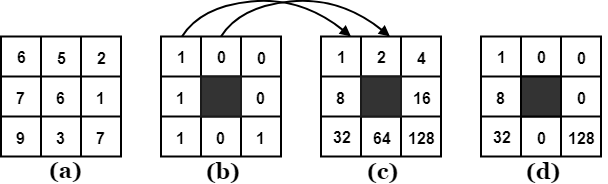
\includegraphics[width=12cm]{figs/LBP2.png}
    \legend{Fonte: Adaptado de \cite{ojala1996comparative}.}
    \label{fig:lbp}
\end{figure}

A~\autoref{fig:lbp} apresenta um exemplo do cálculo LBP. A partir de uma janela de tamanho 3 x 3 (\autoref{fig:lbp} (a)), é realizado a subtração dos valores de níveis de cinza dos \textit{pixels} vizinhos (individualmente) com o valor do nível de cinza do \textit{pixel} central, formando uma matriz binária composta pelos valores 0 ou 1, dependendo do resultado da diferença dos \textit{pixels} analisados (\autoref{fig:lbp} (b)). Em seguida, os valores da matriz binária são multiplicados pelo respectivo valor da matriz de pesos (\autoref{fig:lbp} (c)). Finalmente, o resultado do LBP se dá através da soma de todos os valores resultantes da multiplicação (\autoref{fig:lbp} (d)), no exemplo em questão, o LBP é 169.

\section{Seleção de Características}
\label{sec:selecao}

Em aplicações de visão computacional é bastante recorrente a utilização de técnicas que geram um grande número de características, que muitas vezes são desnecessárias para realizar a separação dos indivíduos em suas classes. Portanto, a escolha do conjunto de características relevantes é importante para simplificar o modelo e aumentar seu poder de generalização. Neste contexto, realiza-se a seleção das características que é uma etapa opcional no processo de reconhecimento de padrões.%, a fim de aumentar a eficiência dos classificadores e diminuir custos computacionais.

A seleção de características visa reduzir a dimensionalidade do espaço de características sem perca de informações. As principais razões para tal redução são os custos de medição e precisão do classificador. Por este motivo, faz-se necessário a utilização de algoritmos de seleção de características que propiciem a obtenção de representações dos padrões de forma robusta. Sendo assim, o algoritmo \textit{Greedy Stepwise} \cite{ambelu2010comparison} foi o escolhido para efetuar este procedimento, afim de aumentar a eficiência dos classificadores e diminuir custos computacionais.

\subsection{Algoritmo \textit{Greedy Stepwise}}
\label{sec:greedyStepwise}

O \textit{Greedy Stepwise} é um algoritmo guloso de paradigma algorítmico que segue a heurística de resolução de problemas de fazer a escolha localmente ótima em cada estágio \cite{gutin2002traveling}, com a intenção de encontrar um ótimo global. Em muitos problemas, uma estratégia gulosa geralmente não produz uma solução ótima. Mesmo assim, uma heurística gananciosa pode produzir soluções ótimas localmente que se aproximam de uma solução globalmente ótima em um período de tempo razoável.

Esse algoritmo executa uma busca gulosa, no sentido \textit{forward} ou \textit{backward}, através do espaço de busca dos subconjuntos de atributos. A busca pode iniciar com nenhum/todos os atributos ou de um ponto arbitrário no espaço, e encerra quando todas as inclusões ou exclusões de atributos resultarem em uma diminuição da taxa de acerto. Para tanto, neste trabalho, esta abordagem encontra características que discriminam melhor as categorias da camada lipídica do filme lacrimal para o conjunto de características geradas, que contém menos redundâncias que poderiam prejudicar os classificadores durante as próximas etapas \cite{ambelu2010comparison}.

\section{Reconhecimento de Padrões}
\label{sec:recPadroes}

O reconhecimento de padrões é o campo da ciência que tem como objetivo a classificação e reconhecimento de objetos em um determinado número de categorias ou classes a partir da observação de suas características \cite{Theodoridis:2008:PRF:1457541}. Dessa forma, visa construir uma representação mais simples de um conjunto de dados através de suas características mais relevantes, possibilitando sua partição em classes \cite{Duda:2000:PC:954544}.

O reconhecimento de padrões tem uma ampla aplicação em astronomia, medicina, robótica, reconhecimento de fala, sensoriamento remoto por satélites, etc. O processo de reconhecimento de padrões é composto por duas etapas: classificação e reconhecimento. Durante a etapa de classificação uma amostra de uma população é particionada em grupos chamados classes. Na etapa de reconhecimento uma amostra desconhecida, porém pertencente à mesma população, é reconhecida como integrante de uma das classes criadas anteriormente \cite{looney1997pattern}.

As técnicas de classificação são compostas por dois grupos: supervisionada e não-supervisionada. A classificação supervisionada consiste em um processo prévio de treinamento de um classificador para o conhecimento dos padrões desejados. Posteriormente, o classificador é capaz de identificar a classe de qualquer objeto desconhecido da mesma população de treinamento. Já na classificação não supervisionada não há informação prévia sobre as classes às quais os padrões de amostras pertencem \cite{pedrini2008analise}.

Neste trabalho foram utilizadas as técnicas de classificação supervisionada \textit{Support Vector Machine}, \textit{Random Forest}, \textit{Naive Bayes} e \textit{Bayes Net} para o reconhecimentos dos padrões de interferência da camada lipídica do filme lacrimal.

\subsection{Classificadores}
\label{sec:classificadores}

O método proposto utiliza \textit{Support Vector Machine} (SVM), \textit{Random Forest} (RF), \textit{Bayes Net} (BN) \cite{nielsen2009bayesian} e \textit{Naive Bayes} (NB) \cite{john2010elements} para o reconhecimento de padrões, objetivando categorizar os padrões de interferência da camada lipídica do filme lacrimal.

%Multilayer Perceptron (MLP) \cite{monika2015di}, Random Tree (RT) \cite{biau2012analysis} e RBFNetwork (RBFNet) \cite{broomhead1988radial}.

A BN pertence à família dos modelos gráficos probabilísticos, que representa um conjunto de variáveis e suas dependências condicionais. Essas estruturas gráficas são usadas para representar o conhecimento sobre um domínio incerto. Particularmente, cada nó no gráfico representa uma variável aleatória, enquanto as arestas entre os nós representam dependências probabilísticas entre as variáveis aleatórias correspondentes. Estas dependências condicionais no gráfico são frequentemente estimadas usando métodos estatísticos e computacionais conhecidos. Assim, as BNs combinam princípios da teoria dos grafos, teoria da probabilidade, ciência da computação e estatística \cite{nielsen2009bayesian}.

%As redes bayesianas são um tipo de modelo gráfico probabilístico que utiliza a inferência bayesiana para cálculos de probabilidade. As redes bayesianas visam modelar a dependência condicional e, portanto, a causalidade, representando a dependência condicional por arestas em um grafo direcionado. Através dessas relações, pode-se conduzir eficientemente a inferência sobre as variáveis aleatórias no gráfico através do uso de fatores.

A NB é um técnica de classificação probabilística baseada no teorema de Bayes com uma suposição de independência entre os preditores, ou seja, as características de cada classe são assumidas como condicionalmente independentes. Por ser muito simples e rápido, possui um desempenho relativamente maior do que outros classificadores. Além disso, o NB precisa apenas de um pequeno número de dados de teste para concluir classificações com uma boa precisão \cite{jensen1996introduction}.

%Naive Bayes é uma técnica simples para a construção de classificadores: modelos que atribuem rótulos de classes a instâncias de problemas, representados como vetores de valores de recursos, em que os rótulos de classes são extraídos de um conjunto finito. 
    
%O RT é baseado na construção de múltiplas árvores de decisão, selecionando subconjuntos aleatórios de variáveis para cada árvore e usando a saída da árvore mais frequente como a classificação geral, ou seja, são geradas uma coleção de árvores de decisão onde cada árvore é formada a partir de diferentes amostras e subconjuntos dos dados de treinamento. A classificação funciona da seguinte maneira: o classificador de árvores aleatórias pega o vetor de recurso de entrada, classifica-o em cada árvore da floresta e exibe o rótulo de classe que recebeu a maioria dos "votos". No caso de uma regressão, a resposta do classificador é a média das respostas sobre todas as árvores na floresta \cite{biau2012analysis}.

O RF é uma técnica baseada na construção de um conjunto de árvores que são classificadores fracos e posteriormente são usados para construir um classificador estável e forte, melhor que a árvore média criada. O RF é um algoritmo flexível que mesmo sem ajuste de hiperparâmetros apresenta um ótimo resultado na maioria das vezes. Além disso, é possível utilizá-lo tanto para tarefas de classificação como de regressão \cite{breiman2001random}. 
    
O SVM é uma técnica baseada na teoria do aprendizado estatístico, usado para encontrar hiperplanos ideais para as classes linearmente separáveis e não separáveis. No segundo caso, são mapeados os dados de entrada para um espaço dimensional superior (usando função do \textit{kernel}) e definido um hiperplano de separação \cite{vapnik1998statistical}. O SVM utiliza o princípio de minimização do risco estrutural, que se baseia no fato de que a taxa de erro de uma máquina de aprendizado nos dados de teste é limitada pela soma da taxa de erro de treinamento e por um termo que depende da dimensão Vapnik-Chervonenkis (dimensão VC) \cite{zhuang2006parameter}.
    
%A MLP é uma abordagem de rede neural que consiste em um sistema de neurônios interconectados simples, ou nós, que mapeiam um conjunto de dados de entrada para um conjunto de saídas apropriadas. A MLP é semelhante à perceptron, mas com mais de uma camada de neurônios em alimentação direta. Tal tipo de rede é composta por camadas de neurônios ligadas entre si por sinapses com pesos. O aprendizado nesse tipo de rede é geralmente feito através do algoritmo de retropropagação do erro \cite{monika2015di}.
    
%A RBFNet permite a escolha do número de clusters (algoritmo de clusterização k-means) e, em seguida, implementa uma função de base radial (atribuição de valores partindo do distanciamento de um centro) para efetuar a classificação. As RBFNets normalmente possuem três camadas: uma camada de entrada, uma camada oculta com uma função de ativação RBF não linear e uma camada de saída linear. A entrada pode ser modelada como um vetor de números reais e a saída da rede é então uma função escalar do vetor de entrada \cite{broomhead1988radial}.

\section{Métricas de Desempenho} 
\label{sec:validacao}

O resultado da etapa de classificação é a identificação das categorias da camada lipídica do filme lacrimal. Após o processo de reconhecimento de padrões existe a necessidade de validar os resultados produzidos, através das métricas de desempenho. Esta atividade tem por finalidade avaliar o desempenho do método desenvolvido por meio de uma análise estatística dos resultados.

Para avaliar o desempenho do método proposto foram utilizadas estatísticas tipicamente aplicadas em sistemas CADx para análise de imagens médicas: acurácia \cite{duda1973pattern}, que é definida como a razão entre o número de casos corretamente classificados pelo número total de casos, e o desvio padrão relacionado a acurácia \cite{viera2005understanding}. Além disso, como existe desequilíbrio entre as classes das categorias, a medida \textit{F-Measure} foi usada, que representa a média harmônica de Precisão e \textit{Recall} \cite{fawcett2006introduction}.

%Além disso, como as classes são desbalanceadas, também usamos F-Measure, que representa a média harmônica de Accuracy e Recall

Outra medida utilizada é o índice \textit{Kappa}, que é um coeficiente de concordância utilizado em escalas nominais. O índice \textit{Kappa} mede a relação entre concordância e causalidade, e também o desacordo esperado, indicando quão legítimas são as interpretações \cite{rosenfield1986coefficient}. Esse índice é recomendado como uma medida que representa integralmente uma matriz de confusão. A categorização dos níveis de acurácia de classificação, pelo índice \textit{Kappa}, pode ser visualizada na~\autoref{tab:indkappa}, conforme definido por \citeonline{landis1977measurement}.

\begin{table}[ht!]
\centering
\rowcolors{1}{}{lightgray}
\onehalfspacing
\caption{Níveis de precisão de classificação, segundo o índice \textit{Kappa}.}
\label{tab:indkappa}
%\resizebox{7.5cm}{!}
\end{table}

O desempenho do método proposto também é avaliado usando a curva ROC (\textit{Receiver Operating Characteristic}), que indica a taxa positiva verdadeira (sensibilidade) como uma função da taxa de falsos positivos (1 - especificidade) \cite{fawcett2006introduction}. A curva é construída variando o limiar do classificador e avaliando os resultados gerados. A principal informação extraída de uma curva ROC é a área sob a curva ROC (\textit{Area Under the ROC Curve} - AUC), quanto maior a área, ou seja, mais próximo de 1 (equivalente a 100\%), melhor é o desempenho do classificador.


\section{Considerações Finais}

Neste capítulo foram apresentadas os fundamentos teóricos que são necessários para compreensão das técnicas utilizadas e suas aplicações no método proposto. Foram abordados temas como: Síndrome do Olho Seco, tipos de imagens do exame, técnicas de pré-processamento digital de imagens, descritores para análise de textura, técnicas para reconhecimento de padrões e métricas de desempenhos.

% detecção de objetos; estimação de pose; panoramas aumentados; aplicações industriais
\chapter{Materiais e Métodos}
\label{metodologia_ref}
\phantom{0}
  
Este capítulo descreve os procedimentos utilizados para diagnóstico dos padrões de interferência da camada lipídica do filme lacrimal, a partir de imagens capturadas com o Interferômetro Doane e Tearscope Plus. Primeiramente são apresentadas as bases de imagens classificadas como um problema multiclasse, nas quais será aplicado o método proposto. Em seguida, é descrita a sequência de etapas realizadas para alcançar o objetivo proposto no método.

\section{Base de Imagens Capturadas com o Interferômetro Doane}
\label{sec:metodoBaseInterferometrica}

A base de imagens VOPTICAL\_GCU \cite{voptical_gcuvarpa2013} contém imagens interferométricas do filme lacrimal, adquiridas de pacientes com a Síndrome do Olho Seco com faixa etária entre 16 e 55 anos. Todas as imagens foram disponibilizadas por dois optometristas do Departamento de Ciências da Vida, da Universidade Caledoniana de Glasgow (Glasgow, Reino Unido).

Nesta base de imagens, a aquisição foi feita usando o Interferômetro Doane \cite{doane1989instrument} e uma câmera digital CMEX-1301. Como o filme lipídico lacrimal não é estático entre os flashes, um vídeo foi gravado e a melhor imagem para processamento foi selecionada. As imagens têm uma resolução de 1280x1024 \textit{pixels} no espaço de cor RGB. A base contém 106 imagens das cinco categorias consideradas: 11 franjas fortes, 25 coalescentes de franjas fortes, 30 franjas finas, 26 coalescentes de franjas finas e 14 detritos. A~\autoref{fig:baseInterferometrica} ilustra exemplos das cinco categorias.

\begin{figure}[ht!]
    \centering
    \caption{Categorias da camada lipídica das imagens da base VOPTICAL\_GCU: (a) franjas fortes; (b) coalescentes de franjas fortes; (c) franjas finas; (d) coalescentes de franjas finas; (e) detritos.}
    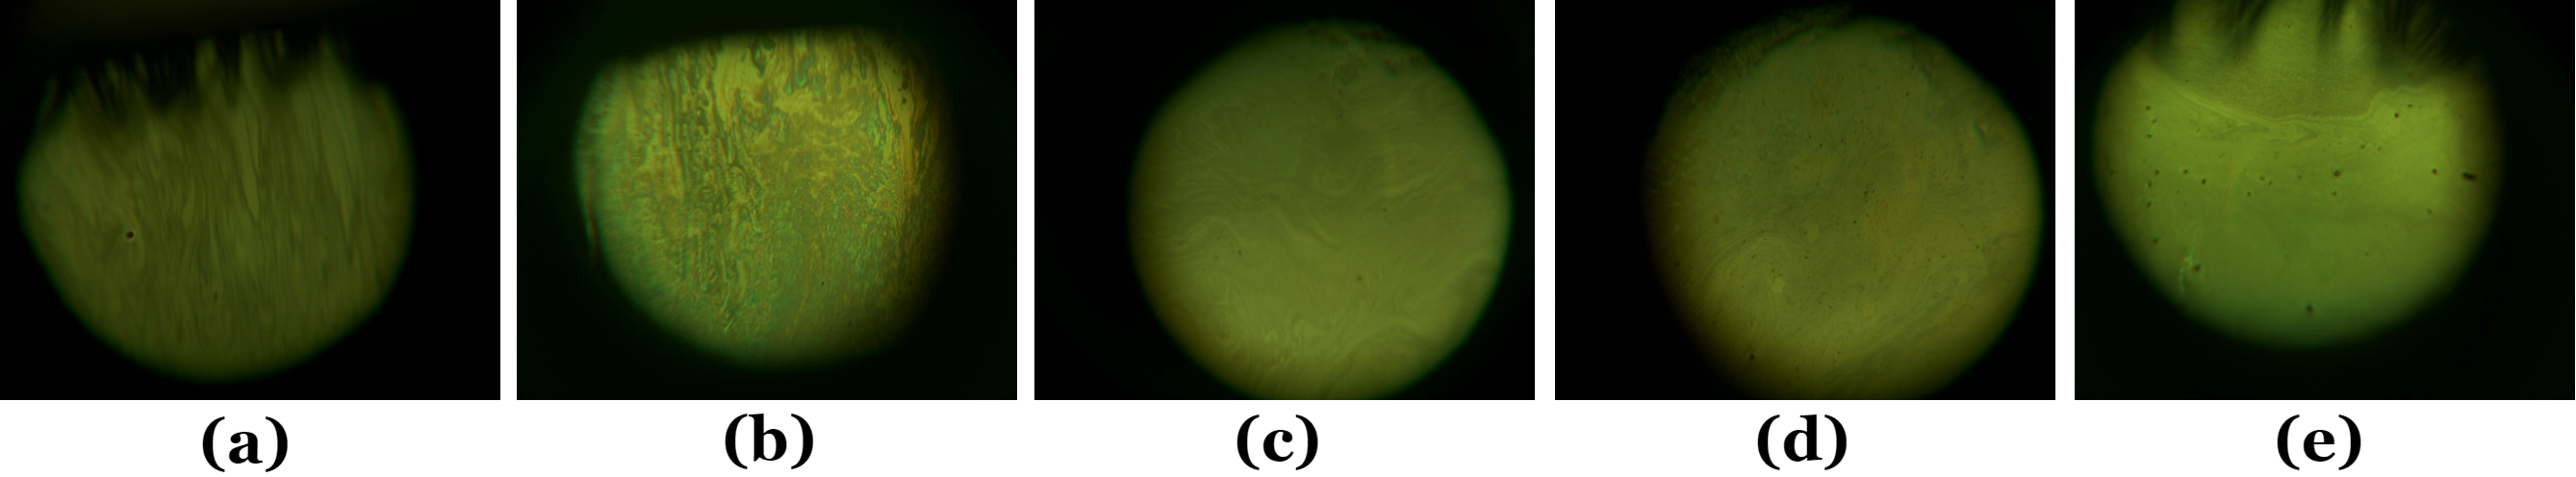
\includegraphics[width=15.8cm]{figs/BaseVOPTICAL.png}
    \legend{Fonte: \cite{voptical_gcuvarpa2013}.}
    \label{fig:baseInterferometrica}
\end{figure}

No estudo realizado por \citeonline{remeseiro2015automatic}, as categorias dos padrões de interferência das imagens foram definidas por optometristas da seguinte forma: (a) franjas óbvias de cor com uma aparência de se espalhar pela córnea; (b) franjas de cores óbvias, mas aglomerando-se em ilhas de cor; (c) franjas cinza com uma aparência de propagação através da córnea; (d) franjas cinza, mas aglomerando-se em ilhas de cinza; e (e) distúrbios óbvios no filme lacrimal, provavelmente de origem variada.

\section{Bases de Imagens Capturadas com o Tearscope Plus}
\label{sec:metodoBaseTearscope}

Os conjuntos de bases VOPTICAL\_I1, VOPTICAL\_I1-v2 e  VOPTICAL\_Is contêm imagens do filme lacrimal pré-ocular adquiridas do mesmo grupo de pacientes com idades entre 19 e 33 anos. A aquisição das imagens foi realizada com o Tearscope Plus (Keeler Ltd., Reino Unido)  \cite{guillon1997tearscope} acoplado a uma lâmpada de fenda Topcon SL-D4 e uma câmera digital Topcon DV-3. Um vídeo foi gravado e a melhor imagem foi selecionada. Todas as imagens têm uma resolução de 1024x768 \textit{pixels} e estão no espaço de cor RGB. Estes conjuntos de imagens foram adquiridos e anotados por optometristas do Serviço de Optometria da Universidade de Santiago de Compostela (Espanha).

O Tearscope Plus permite aos médicos avaliar rapidamente a espessura da camada lipídica. \citeonline{guillon1998non} definiu uma escala de classificação composta de cinco categorias, que em espessura crescente são: malha aberta, malha fechada, onda, amorfa e franja de cor.

%O tacoplado a uma lâmpada de fenda Topcon SL-D4 e uma câmera digital Topcon DV-3. A ampliação do biomicroscópio foi ajustada para 200X e as imagens armazenadas com uma resolução de 1024 768 pixels. Como o lípide lacrimal lm não é estático entre os flashes, um vídeo foi gravado e analisado para selecionar as imagens a serem processadas: uma imagem foi selecionada somente quando o lípide do lípido lacrimal foi completamente expandido após o piscar do olho.

%O Tearscope Plus, projetado por Guillon [1], é o instrumento de escolha para a avaliação da espessura da camada lipídica em ambientes clínicos. Guillon também propôs cinco principais categorias de lipídios

%Guillon também propôs cinco graus principais de padrões de interferência da espessura da camada lipídica para observações feitas usando o Tearscope Plus: malha aberta (10–20 nm), malha fechada (20–50 nm), onda (50–70 nm), amorfa (80–90 nm) e cor de franja (90–180 nm). Outros padrões associados à patologia ocular frequentemente aparecem como franjas anormais de cor, referidas como padrões globulares (> 180 nm).

%Observe que a espessura da camada lipídica está associada aos olho SF, pois uma camada lipídica mais fina acelera a evaporação da água.
%Os nomes dos arquivos das imagens indicam o padrão de interferência predominante: CO é franja de cor, AM é amorfo, FL é onda, MA é malha aberta e MC é malha fechada.

\subsection{Bases VOPTICAL\_I1 e VOPTICAL\_Is}
\label{subsec:basesI1eIs}

Embora os padrões de interferência sejam independentes da iluminação, existe uma faixa ótima de iluminações usadas pelos optometristas para obter as imagens. Imagens com iluminações fora deste intervalo são consideradas imagens ruidosas \cite{remeseiro2014methodology}. Dessa maneira, dois conjuntos de imagens foram gerenciados. A primeira base contém 105 imagens do conjunto VOPTICAL\_I1 \cite{voptical_gcuvarpa_i1}, todas nas mesmas condições de iluminação, distribuídas em 29 malhas abertas, 29 malhas fechadas, 25 de ondas e 22 de franja de cor.

A segunda base contém 406 imagens do conjunto de imagens VOPTICAL\_Is \cite{voptical_gcuvarpa_is}, em diferentes condições de iluminação. Esta base possui 159 malhas abertas, 117 malhas fechadas, 90 ondas e 40 franja de cor. Não contém imagens dentro da categoria amorfa porque é um padrão muito incomum \cite{garcia2013new}, e por esta razão a última categoria não foi considerada nessas duas bases.

A~\autoref{fig:2basesTeascope} mostra exemplos de imagens das categorias da camada lipídica em ambas as bases. As imagens superiores compõem a base VOPTICAL\_I1, e as inferiores a base VOPTICAL\_Is. As imagens da base VOPTICAL\_Is possuem uma iluminação muito alta, produzindo uma imagem onde o padrão de interferência é dificilmente apreciado.

\begin{figure}[ht!]
    \centering
    \caption{Categorias da camada lipídica. Imagens superiores são da base VOPTICAL\_I1 e inferiores VOPTICAL\_Is: (a) malhas abertas; (b) malhas fechadas; (c) ondas; (d) franja de cor.}
    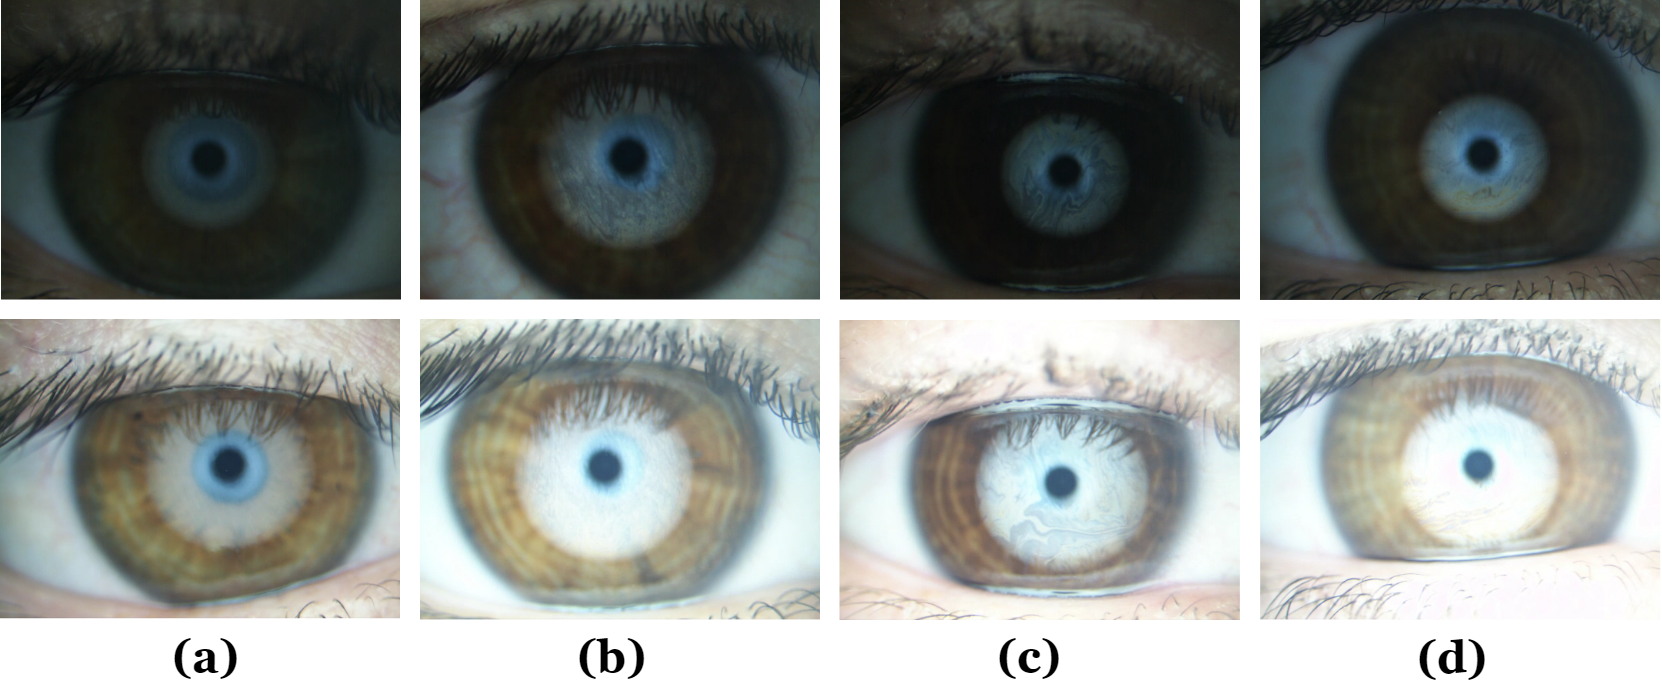
\includegraphics[width=15.4cm]{figs/DuasBases1.png}
    \legend{Fonte: \cite{voptical_gcuvarpa_i1, voptical_gcuvarpa_is}.}
    \label{fig:2basesTeascope}
\end{figure}

\subsection{Base VOPTICAL\_I1-v2}

O conjunto de imagens VOPTICAL\_I1-v2 \cite{voptical_gcuvarpa_i1-v2} é a versão atualizada do conjunto de imagens VOPTICAL\_I1 e inclui a categoria amorfa. A base contém 128 imagens do filme lacrimal adquiridas de pacientes com olhos escuros. O conjunto de imagens têm 29 malhas abertas, 29 malhas fechadas, 25 ondas, 23 amorfas e 22 franja de cor. A~\autoref{fig:basesVersao2Teascope} demonstra exemplos das cinco categorias da camada lipídica.

\begin{figure}[ht!]
    \centering
    \caption{Categorias da camada lipídica das imagens da base VOPTICAL\_I1-v2: (a) malhas abertas; (b) malhas fechadas; (c) ondas; (d) amorfas; (e) franja de cor.}
    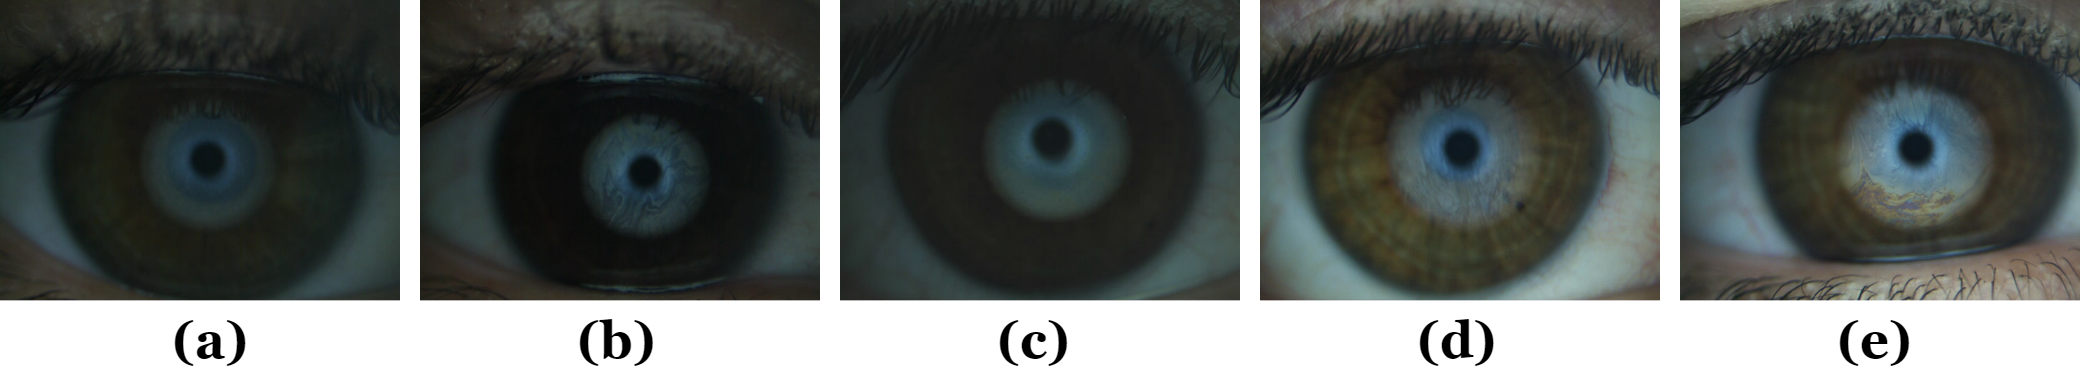
\includegraphics[width=15.8cm]{figs/BaseVersao2.png}
    \legend{Fonte: \cite{voptical_gcuvarpa_i1-v2}.}
    \label{fig:basesVersao2Teascope}
\end{figure}

\section{Método Proposto}
\label{sec:metodoProposto}

%O método proposto consiste em quatro etapas: segmentação, extração de características, seleção de características e reconhecimento de padrões. A~\autoref{fig:metodoProposto} ilustra a sequência que essas etapas são executadas. Na primeira etapa é realizado a segmentação das quatro bases de imagens, uma capturada com o Interferômetro Doane e três com o Teascope Plus. Na segunda etapa é realizado a extração de características com os descritores de textura baseados em índices de diversidade filogenéticos, que são aplicados somente nas imagens capturadas com o Interferômetro Doane, e a função K de \textit{Ripley} nas imagens capturadas com o Teascope Plus.

%As características mais discriminantes dos vetores de características extraídos são selecionados na terceira etapa e, submetidos como entrada para o processo de classificação supervisionada (quarta etapa) usando os classificadores Random Forest, SVM, Naive Bayes e Bayes Net. Finalmente, os resultados são validados utilizando métricas de desempenho e comparados com os resultados encontrados na literatura.

%O método proposto consiste em quatro etapas: segmentação, extração de características, seleção de características e reconhecimento de padrões. Foram realizados testes separadamente para cada base de imagens, a Seção~\ref{sec:resultadosDisc} apresentará os resultados obtidos em cada um dos experimentos. Para cada tipo de base de imagens, os fluxos apresentam sequências diferentes em algumas etapas. A~\autoref{fig:metodoProposto} ilustra a sequência que as etapas são executadas.

%O método proposto consiste em quatro etapas: segmentação, extração de características, seleção de características e reconhecimento de padrões. Para cada tipo de base de imagens, os fluxos apresentam sequências diferentes em algumas etapas e, consequentemente, serão apresentados os resultados para os diferentes tipos de bases de imagens. A~\autoref{fig:metodoProposto} ilustra a sequência que as etapas são executadas.

O método proposto consiste em quatro etapas: segmentação, extração de características, seleção de características e reconhecimento de padrões. A~\autoref{fig:metodoProposto} ilustra a sequência que as etapas são executadas. Para cada tipo de base de imagens, os fluxos apresentam sequências diferentes em algumas etapas, e são realizados testes separadamente para cada base de imagens, o Capítulo~\ref{sec:resultadosDisc} apresentará os resultados obtidos em cada um dos experimentos.

Na primeira etapa realiza-se a segmentação da região de interesse nas imagens das quatro bases, uma capturada com o Interferômetro Doane e três com o Tearscope Plus. Na segunda etapa é realizado a extração de características com os descritores de textura baseados em índices de diversidade filogenética, que são aplicados nas imagens da base capturada com o Interferômetro Doane; e a função K de \textit{Ripley} nas imagens das bases capturadas com o Tearscope Plus e Interferômetro Doane.

As características mais discriminantes dos vetores de características extraídos são selecionadas na terceira etapa para todas as bases de imagens, posteriormente, são submetidas como entrada para o processo de classificação supervisionada (quarta etapa) usando os classificadores \textit{Random Forest}, \textit{Support Vector Machine}, \textit{Naive Bayes} e \textit{Bayes Net}. Finalmente, os resultados obtidos são validados utilizando métricas de desempenho e comparados com os resultados encontrados na literatura.

%As características mais discriminantes dos vetores de características extraídos são selecionados na terceira etapa e, submetidos como entrada para o processo de classificação supervisionada (quarta etapa) usando os classificadores Random Forest, SVM, Naive Bayes e Bayes Net. Finalmente, os resultados são validados utilizando métricas de desempenho e comparados com os resultados encontrados na literatura.

\begin{comment}
O método proposto consiste em quatro etapas: segmentação, extração de características, seleção de características e reconhecimento de padrões. A~\autoref{fig:metodoProposto} ilustra a sequência que as etapas são executadas para o fluxo (1) que utiliza base de imagem capturada com o Interferômetro Doane; e o fluxo (2) bases de imagens capturadas com o Tearscope Plus. Pode ser observado que os fluxos (1) e (2) apresentam sequências diferentes em algumas etapas e, consequentemente, serão apresentados os resultados para os diferentes fluxos.

Em geral, a primeira etapa é realizado a segmentação da região de interesse nas quatro bases de imagens, em que uma base é capturada com o Interferômetro Doane e três com o Tearscope Plus. Na segunda etapa é realizado a extração de características com os descritores de textura baseados em índices de diversidade filogenética no fluxo (1), e a função K de \textit{Ripley} no fluxo (1) e (2).

As características mais discriminantes dos vetores de características extraídos são selecionados na terceira etapa em ambos os fluxos e, submetidos como entrada para o processo de classificação supervisionada (quarta etapa) usando os classificadores \textit{Random Forest}, \textit{Support Vector Machine}, \textit{Naive Bayes} e \textit{Bayes Net}. Finalmente, os resultados dos fluxos são validados utilizando métricas de desempenho e comparados com os resultados encontrados na literatura.
\end{comment}

\begin{figure}[ht!]
    \centering
    \caption{Etapas do método proposto.}
    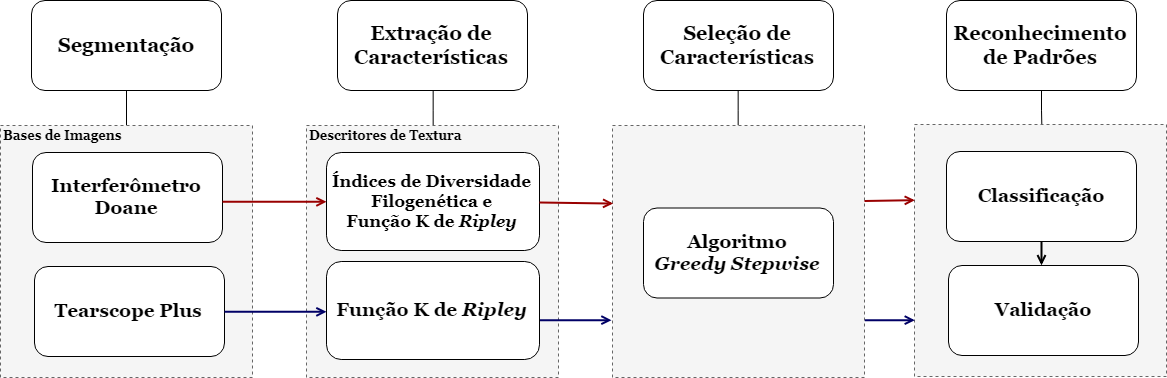
\includegraphics[width=15.8cm]{figs/metodoDissertacao2.png}
    \legend{Fonte: Elaborado pela autora.}
    \label{fig:metodoProposto}
\end{figure}

\subsection{Segmentação}
\label{sec:metodoSegmentacao}

%A segmentação consiste na separação dos objetos de interesse de informações irrelevantes presentes em imagens digitalizadas. As Seções seguintes apresentam duas segmentações diferentes referentes as quatro bases de imagens, divididas em dois grupos de tipos de imagens, utilizando o Interferômetro Doane (base VOPTICAL\_GCU) e o Tearscope Plus (base VOPTICAL\_I1, VOPTICAL\_I1-v2 e VOPTICAL\_LS).

A segmentação consiste na separação dos objetos de interesse, de informações irrelevantes presentes em imagens digitalizadas. As seções seguintes apresentam duas segmentações diferentes referentes aos tipos de imagens capturadas com o Interferômetro Doane (base VOPTICAL\_GCU) e as capturadas com Tearscope Plus (base VOPTICAL\_I1, VOPTICAL\_I1-v2 e VOPTICAL\_Is).


%Na segmentação manual todo o processo de separação de um objeto de interesse é conduzido por um especialista humano, o que torna o procedimento exaustivo e custoso. Portanto, faz-se necessário um sistema para segmentação automática das regiões de interesse, visando tornar o trabalho ágil e menos custoso. Nesta dissertação foram utilizadas quatro bases de imagens, e realizadas duas segmentação diferentes para os tipos de imagem que compõem as bases. A seguir são detalhados tais procedimentos.

\subsubsection{Segmentação das ROIs de Imagens Capturadas pelo Interferômetro Doane}
\label{sec:metodoSegInterferometroDoane}

As imagens de entrada adquiridas com o Interferômetro Doane, incluem áreas irrelevantes presentes nas áreas externas, como ilustrado na~\autoref{fig:ExtracaoROI} (a). Assim, a região mais relevante para segmentação encontra-se na parte central da área amarelada ou esverdeada da imagem, formada pela superfície anterior do filme lacrimal que cobre a córnea. Portanto, foi realizado um passo destinado à extração da ROI, conforme proposto em \cite{remeseiro2015automatic}.

\begin{figure}[ht!]
    \centering
    \caption{Etapas da segmentação da ROI de imagens capturadas com Interferômetro Doane.}
    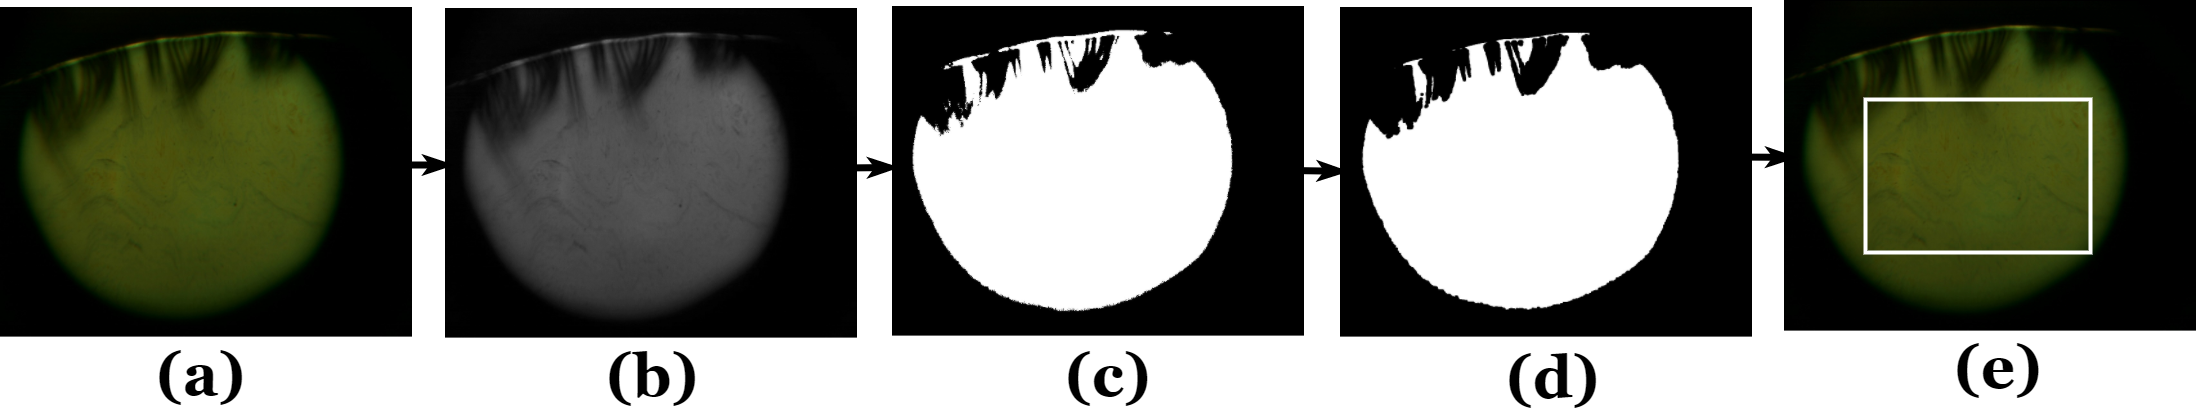
\includegraphics[width=15.8cm]{figs/ExtracaoROI.png}
    \legend{Fonte: Elaborado pela autora.}
    \label{fig:ExtracaoROI}
\end{figure}

A região relevante da imagem é caracterizada por tonalidades esverdeadas ou amareladas, assim apenas o canal verde (G) da imagem de entrada em RGB é considerado (\autoref{fig:ExtracaoROI} (b)). Na imagem do canal G é usado o princípio de limiar, que consiste em separar os \textit{pixels} da imagem em duas classes (fundo e objeto). O objetivo é encontrar os \textit{pixels} cujo nível de cinza é menor que um limite (\autoref{fig:ExtracaoROI} (c)). O cálculo desse limite é apresentado na~\autoref{equacao:equacaoLimiar}.

\begin{equation}
\label{equacao:equacaoLimiar}
limiar = media - p  \times \sigma,
\end{equation}onde $media$ constitui o valor médio dos níveis de cinza da imagem, $\sigma$ é o desvio padrão e $p$ é um fator de peso empiricamente determinado ($p$ = 0,1). Depois que a ROI preliminar é identificada, sua parte central deve ser localizada. Devido algumas imagens incluírem outras regiões irrelevantes, como cílios, o operador morfológico de erosão \cite{gonzalez2008digital}, usando uma elipse como elemento estruturante é aplicado (\autoref{fig:ExtracaoROI} (d)). Em seguida, um retângulo dentro da região identificada acima é mapeado e reduzido até que nenhuma área do fundo permaneça (\autoref{fig:ExtracaoROI} (e)). Observa-se que o tamanho das imagens de entrada é 1280 x 1024 \textit{pixels}, e o tamanho final da ROI é, em média, 547 x 578 \textit{pixels}.

%Especialistas geralmente se concentram na parte inferior da íris, porque esta é a área onde a lágrima pode ser percebida com o melhor contraste.

\subsubsection{Segmentação das ROIs de Imagens Capturadas pelo Tearscope Plus}
\label{sec:metodoSegTearscopePlus}

As imagens de entrada obtidas com o Tearscope Plus, incluem várias áreas do olho que não contêm informações relevantes para a classificação, conforme ilustrado na~\autoref{fig:ExtracaoROI2} (a). O procedimento de aquisição garante que há uma área central na imagem mais iluminada do que o ambiente ao redor, na qual o filme lacrimal pode ser observado. Consequentemente, optometristas que analisam visualmente essas imagens concentram sua atenção nessa parte da íris, ou seja, na área mais clara entre a pupila e o limite da íris. Portanto, este fato força uma etapa destinada a extração da ROI.

%O procedimento de aquisição garante que esta região corresponda à área mais iluminada da imagem. Para isso, a imagem de entrada é transformada no espaço de cores Lab e somente o componente L é considerado nesta etapa. Além disso, um conjunto de modelos em forma de anel que definem diferentes formas de ROI é usado. Em seguida, a correlação cruzada normalizada entre o componente L e o conjunto de modelos é calculada. Finalmente, a região com o valor máximo de correlação cruzada é selecionada [ver Figura 3 (b)] e a ROI da imagem de entrada é obtida através de um processo completamente automático.

\begin{figure}[ht!]
    \centering
    \caption{Etapas da segmentação da ROI de imagens capturadas com Tearscope Plus.}
    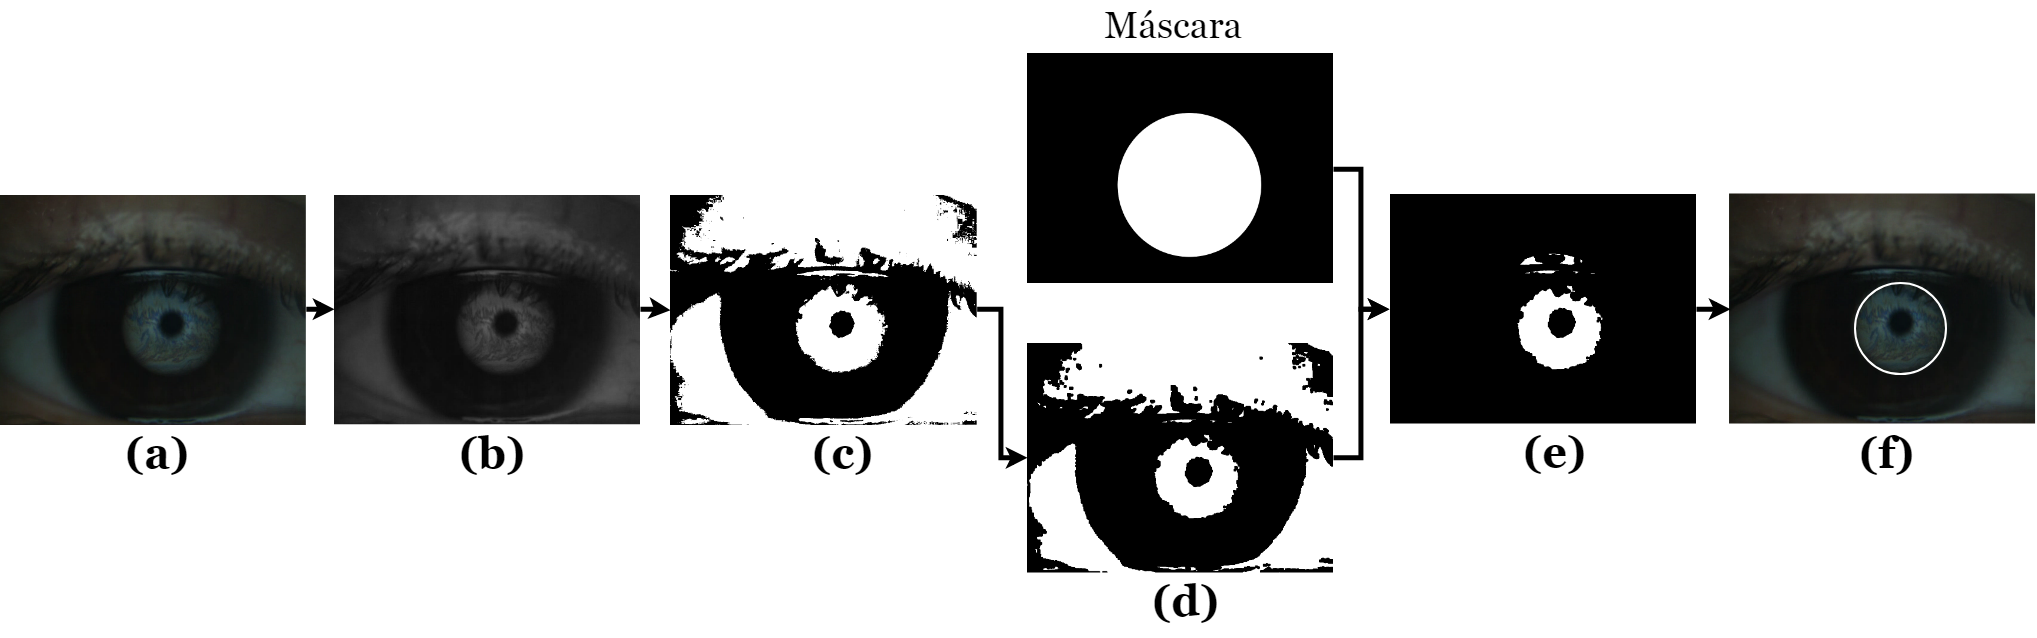
\includegraphics[width=15.8cm]{figs/ExtracaoROI3.png}
    \label{fig:ExtracaoROI2}
    \legend{Fonte: Elaborado pela autora.}
\end{figure}

O filme lacrimal pode ser percebido com o maior contraste no canal verde da imagem de entrada, assim como nas imagens interferométricas. Portanto, as etapas apresentadas na \autoref{fig:ExtracaoROI2} (b), (c) e (d) seguem os mesmos procedimentos encontrados nas etapas da~\autoref{fig:ExtracaoROI} (b), (c) e (d) detalhadas na Subseção~\ref{sec:metodoSegInterferometroDoane}. Em seguida, foi observado que a região de interesse encontra-se sempre um pouco abaixo do centro das imagens. Assim, uma máscara fixa foi utilizada nesta etapa, extraindo apenas as informações que coincidem com a região marcada pela máscara fixa (\autoref{fig:ExtracaoROI2} (e)). Uma vez identificada esta ROI preliminar, pode ser observado que algumas imagens ainda incluem outras regiões que não contêm informações relevantes para a extração de características. Para eliminar essas regiões foram localizadas circunferências no objeto de interesse. Por fim, foi retornado a circunferência que contém maior área, representando a região de interesse para extração de características (\autoref{fig:ExtracaoROI2} (f)).

\subsection{Extração de Características}
\label{sec:metodoExtracao}

Após a extração da ROI, inicializa-se a etapa de caracterização. Esta etapa visa obter medidas descritivas da camada lipídica do filme lacrimal, que formarão os vetores de características a serem utilizados nas etapas de seleção e classificação. O procedimento de extração de características adotado neste trabalho é distribuído em análises de texturas baseadas em geoestatística (Subseção~\ref{sec:kripley}) e índices de diversidade filogenética (Subseção~\ref{sec:indicesDiversidade}). %\cite{doi:10.2989/16085910409503825}

Nas bases de imagens capturadas com o Interferômetro Doane são aplicados os descritores baseados em índices de diversidade filogenética e a função K de \textit{Ripley}. E nas bases capturadas com o Tearscope Plus são aplicadas a função K de \textit{Ripley}. A seguir, são detalhadas as adaptações utilizadas para a extração de características com essas técnicas.

\subsubsection{Extração de Características usando a Função K de \textit{Ripley}}
\label{sec:metodoRipley}

Os índices geostatísticos descrevem a textura em termos de medidas de autocorrelação espacial. A autocorrelação espacial é uma medida de similaridade entre pontos em uma certa distância \cite{clark1979practical}. Especificamente, no contexto deste descritor, é utilizada a representação da ROI em LBP padrão com tamanho de janela $3x3$, onde um ponto analisado em geostatística corresponderá ao padrão binário local na ROI, aplicado sobre os espaços de cores baseado em cores oponentes, L*a*b*, RGB e YCbCr \cite{plataniotis2013color}.

Posteriormente, são aplicadas as abordagens em círculos e anéis apresentadas sobre a função K de \textit{Ripley} (Subseção~\ref{sec:kripley}). O procedimento adotado é semelhante para as duas abordagens. Para diferentes valores de raios $r$, a partir da escolha de um centro $i$, são analisadas as ocorrências de LBPs de um mesmo valor $j$. Foram utilizados 6 raios, parâmetro empiricamente testado, onde valores menores normalmente reduzem o desempenho e valores maiores aumentam a complexidade e não incluem características relevantes. Vale observar que a escolha da quantidade de raios é um critério dependente da abordagem adotada e pode variar entre métodos ou estudos diferentes.

Para determinar os 6 raios é necessário calcular o raio máximo que pode ser alcançado a partir do seu centro, ou seja, a distância entre o centro da ROI até o \textit{pixel} mais distante pertencente à mesma (cálculos apresentados na Seção~\ref{sec:kripley}). A quantidade de raios provê uma divisão das ROIs em círculos ou anéis de tamanhos que crescem gradativamente em variação relativamente pequena de raio, mas não unitária. %Cada raio é definido através da equação:

\begin{comment}
\begin{equation}
\label{equacao:raioRipley}
R_{i} = \frac{R_{Max}}{6}*i \ \ \ \ \ \ \ para \ \ \ i = 1,2,3,4,5,6
\end{equation}
\end{comment}

Além da utilização dos raios, pretende-se encontrar características existentes em agrupamentos de um mesmo padrão, com o objetivo de representar a maior quantidade possível de informações sobre as camadas lipídicas. Para atingir este objetivo, cada ROI foi quantizada sucessivamente de 256 níveis, para 128, 64, 32, 16 e 8, que corresponde a 6 quantizações diferentes para cada um dos 6 raios de amostragem. Além disso, vale ressaltar que foram realizados experimentos exaustivos de quantização e foram apresentados apenas os melhores resultados.

Posteriormente, o LBP foi aplicado sobre o resultado de cada uma das quantizações. Finalmente, cada raio de amostragem gera uma observação sobre cada um dos 3 canais de cada espaço de cores. Dessa forma, são extraídas 3024 características (6 raios x (256 + 128 + 64 + 32 + 16 + 8 quantizações)) para cada canal de cada espaço de cor, totalizando 9072 características.

\subsubsection{Extração de Características usando Índices de Diversidade Filogenética}
\label{sec:metodoIndicesD}

Para descrição da textura, foram utilizados todos os índices de diversidade filogenética apresentados na Seção~\ref{sec:indicesDiversidade}. Esse descritor de textura foi utilizado somente na base de imagens capturadas com os Interferômetro Doane (Subseção~\ref{sec:metodoBaseInterferometrica}) e aplicado sobre o espaço de cor em nível de cinza.

O processo de extração de características usando os índices de diversidade filogenética é semelhante em todos os grupos dos índices filogenéticos. Esses índices são utilizados para analisar a distribuição de espécies em uma região de análise, usados em conjunto com as árvores filogenéticas. Para montar e organizar
a árvore, é necessário saber quais espécies estão presentes na ROI, sendo elas representadas pelos níveis de cinza dos \textit{pixel} em cada ROI da camada lipídica.

Como explicado na Seção~\ref{sec:indicesDiversidade}, as árvores filogenéticas são usadas na biologia para descrever as relações evolutivas entre as espécies. Nessas árvores, as folhas representam as espécies e os nós internos representam os antepassados comuns à espécie. Assim, é possível fazer uma conexão evolucionária entre as espécies estudadas. O cladograma (\autoref{fig:Cladograma}) foi a representação gráfica usada para descrever a relação filogenética entre espécies e seus antepassados \cite{vane1991protect}.

A partir do cladograma, foi adaptado o conceito de árvores filogenéticas para o contexto de processamento de imagens. A comunidade foi representada pela ROI, seus indivíduos pelos \textit{pixels}, os níveis de cinza as suas espécies, os ancestrais são os nós internos no cladograma, e a distância filogenética o número de arestas entre duas espécies. Com isso, os índices de diversidade filogenética foram calculados para aferir as relações filogenéticas entre as espécies
existentes na comunidade \cite{carvalho2016metodos,vane1991protect}.

\subsection{Seleção de Características}
\label{sec:metodoSelecaoC}

Esta etapa foi introduzida no método devido as duas abordagens da função K de \textit{Ripley} gerarem um número muito grande de variáveis, sendo que muitas poderiam ser redundantes e com isso diminuir a eficiência do classificador. Em outras palavras, o objetivo dessa etapa é encontrar um subconjunto de medidas, de modo a diminuir a dimensionalidade, eliminando variáveis redundantes e, dessa forma, melhorar a eficiência do processo de classificação.

Para efetuar este processo, foi utilizado o Algoritmo \textit{Greedy Stepwise} apresentado na Seção~\ref{sec:greedyStepwise}. Esse algoritmo consiste em uma sequência de passos iterativos, onde o início é dado por uma configuração de solução arbitrária qualquer. Os demais passos trocam uma das variáveis da solução dada na etapa anterior à procura de uma melhor taxa de acerto. Se a troca resultou em sucesso, a nova melhor taxa é anotada. A repetição iterativa acontece até que não ocorra alteração de melhor taxa de acerto. Assim, espera-se que o conjunto de características resultante possa conter menos variáveis redundantes, as quais poderiam prejudicar o classificador durante as próximas etapas.

\subsection{Reconhecimento de Padrões}
\label{sec:metodoReconhecimentoP}

Nesta etapa são apresentadas as técnicas utilizadas na etapa de reconhecimento de padrões. Por meio de experimentos de classificação, esta fase visa analisar se as características produzidas são capazes de diferenciar os padrões de interferência da camada lipídica do filme lacrimal.

\subsubsection{Classificação}
\label{sec:metodoClassificacao}

Conforme descrito na Seção~\ref{sec:classificadores}, o objetivo desta etapa consiste em classificar categorias dos padrões de interferência da camada lipídica do filme lacrimal, a partir dos vetores de características produzidos na etapa anterior.

Após obter a base de características, inicia-se o processo de reconhecimento de padrões pela normalização dos dados. Este processo tem como objetivo padronizar a distribuição dos valores das características para uma faixa de valores entre 0 e 1. A normalização dos dados também é utilizada para auxiliar o classificador a convergir com maior facilidade durante a etapa de treinamento \cite{duda1973pattern}.

Finalizando a normalização, a base de características foi dividida em dois conjuntos: uma para treino e outra para teste. Pelo fato do conjunto de teste ser, na maioria das vezes, menor que o conjunto de treinamento, há o risco deste não ser suficientemente representativo para todo o conjunto, e portanto, a avaliação feita ser ruidosa. A fim de evitar isto, a estratégia de validação cruzada \textit{k-fold} foi usada \cite{rodriguez2010sensitivity}. 

%A validação cruzada foi definida o número de k-fold = 10, sendo computados seus valores médios para todas as métricas (Seção~\ref{sec:validacao}) após a execução de cinco classificações aleatória, com o objetivo de verificar a consistência dos resultados. Em outras palavras, a repetição dos experimentos busca analisar se a função de classificação sofre grandes variações a cada experimento.

Foram definidos 10 \textit{folds} na validação cruzada. Com o objetivo de verificar a consistência dos resultados, foi executada o mesmo procedimento cinco vezes com classificações aleatórias e, posteriormente foram computados seus valores médios para todas as métricas (Seção~\ref{sec:validacao}). Portando, a repetição dos experimentos buscou analisar se a função de classificação sofreu grandes variações a cada experimento, e também demonstrar que o método é robusto as mais diversas situações.

A função de núcleo utilizada no SVM foi a função de base radial, também chamada \textit{kernel} RBF \cite{scholkopf2002learning}. Devido a natureza aleatória da divisão da base, foram estimados em cada experimento os parâmetros $C$ e $\gamma$, que representam o custo, e o grau de complexidade da função de mapeamento, respectivamente. Os parâmetros foram estimados para cada \textit{k-fold} através do \textit{Grid-Search} que é fornecido no pacote LIBSVM \cite{chang2011libsvm}.

Os outros classificadores foram usados com a configuração padrão do WEKA 3.8 \cite{hall2009weka}. Foi usado distribuição normal nos atributos numéricos para NB, e discretização supervisionada para converter atributos numéricos para valores nominais; no RF não foi definido nenhum valor para a profundidade máxima da árvore e foram utilizadas trezentas iterações; e o método K2 \cite{cooper1992bayesian} foi o utilizado para pesquisar estruturas da rede no BN.

\subsection{Validação dos Resultados}
\label{sec:metodoValidacao}

Após a conclusão da etapa de reconhecimento de padrões, é necessário validar e discutir os resultados dos experimentos. Este processo é realizado utilizando métricas comumente aplicadas em sistemas CAD/CADx. As métricas utilizadas foram: acurácia, desvio padrão em relação a acurácia, \textit{F-Measure}, \textit{Kappa} e curva ROC (Seção~\ref{sec:validacao}). A etapa de validação dos resultados tem como objetivo medir o desempenho do método proposto e também discriminar seus pontos positivos e negativos, para que possa buscar melhorias em trabalhos futuros.

\section{Considerações Finais}
\label{sec:metodoConsideracoesF}

Este capítulo apresentou e descreveu, minuciosamente, o método proposto para classificação da camada lipídica em imagens do filme lacrimal. Foram detalhadas cada uma das etapas que compõem o método, e apresentadas as adaptações empregadas para utilização dos descritores de textura propostos nesta dissertação.

No próximo capítulo serão apresentados os resultados obtidos a partir da aplicação do método proposto. Será feita uma discussão acerca dos resultados obtidos, e também uma comparação com os trabalhos descritos na literatura, visando contextualizar a relevância da pesquisa desenvolvida neste trabalho.
% marcador natural; estimação de pose; 
\chapter{Resultados e Discussão}
\phantom{0}
\label{sec:resultadosDisc}

Nesta seção são apresentados e detalhados os resultados dos experimentos realizados para validação do método proposto. Destaca-se que o propósito dos experimentos é investigar a aplicabilidade dos descritores de textura e os classificadores explorados nesta dissertação. Em outras palavras, o objetivo é identificar o conjunto de características que mais contribua para a classificação das categorias da camada lipídica do filme lacrimal. Além disso, é realizada uma discussão a respeito dos resultados obtidos, e uma análise comparativa (Seção~\ref{sec:comparacao}) com os trabalhos relacionados (Seção~\ref{sec:trabRelacionados}).

Os resultados estão organizados de acordo com a técnica utilizada. Na função K de \textit{Ripley} as ROIs são analisadas nos espaços de cores baseados em cores oponentes (CO), YCbCr, RGB e L*a*b*, e nos índices de diversidade filogenética em escala de cinza. Os valores apresentados representam a média das 5 repetições na validação cruzada (\textit{k-fold} = 10). São apresentadas as médias de acurácia (AC), desvio padrão em relação a acurácia (DP), \textit{Kappa}, \textit{F-Measure} (FM) e a curva ROC, destacando-se o melhor resultado em cada experimento.


\section{Experimentos utilizando a Função K de \textit{Ripley}} 
\label{sec:expKRipley}

Esta seção apresenta e discute os resultados obtidos aplicando as abordagens em círculos e anéis apresentadas sobre a função K de \textit{Ripley}. Essa técnica é realizada nas imagens das bases capturadas com o Tearscope Plus e o Interferômetro Doane.

Conforme descrito na Seção~\ref{sec:kripley}, as abordagens em círculos e anéis usando a função K de \textit{Ripley} geram 3024 características (6 raios e 6 quantizações, sendo a quantidade de variáveis de cada raio igual a 504 (254 + 128 + 64 + 32 + 16 + 8)) para cada um dos três canais de um espaço de cor, totalizando um conjunto de 9072 características. Devido à grande quantidade de variáveis extraídas, o algoritmo de seleção \textit{Greedy Stepwise} foi utilizado para reduzir a dimensionalidade, e aumentar a eficiência dos classificadores. Ciente disso, a seguir são apresentados os resultados produzidos para cada base de imagens utilizada.

\subsection{Resultados sobre as Imagens das Bases Capturadas com o Tearscope Plus}

As subseções seguintes são dedicadas para apresentar os resultados obtidos aplicando a função K de \textit{Ripley} sobre as imagens das bases VOPTICAL\_I1, VOPTICAL\_I1-v2 e VOPTICAL\_Is capturadas com o Tearscope Plus.

\subsubsection{Resultados da Base VOPTICAL\_I1}

A Tabela~\ref{tab:cirVOPTICAL_I1} apresenta a aplicação da abordagem em círculos sobre a função K de \textit{Ripley}. A maior taxa de acerto foi obtida no espaço de cor (EC) YCbCr, utilizando o classificador BN após o processo de seleção de características pelo \textit{Greedy Stepwise}, resultando em 92 variáveis selecionadas (VS). O resultado apresenta 99,23\% de acurácia, 0,79\% de desvio padrão sobre a acurácia, 0,99 de área sob a curva ROC, 0,98 de \textit{Kappa} e 0,99 de \textit{F-Measure}.

\definecolor{lightgray2}{gray}{0.8}
\begin{table}[!ht]
\centering
\onehalfspacing
\caption{Resultados produzidos sobre a base VOPTICAL\_I1, aplicando a função K de \textit{Ripley} usando abordagem em círculos.}
\label{tab:cirVOPTICAL_I1}
\resizebox{13cm}{!}{%
\begin{tabular}{llcccccc}
\cline{2-8}
 & \textbf{EC} & \multicolumn{1}{l}{\textbf{AC(\%)}} & \multicolumn{1}{l}{\textbf{DP(\%)}} & \multicolumn{1}{l}{\textbf{ROC}} & \multicolumn{1}{l}{\textbf{\textit{Kappa}}} & \multicolumn{1}{l}{\textbf{FM}} & \multicolumn{1}{l}{\textbf{VS}} \\ \cline{2-8} \parbox[t]{4mm}{\multirow{4}{*}{\rotatebox[origin=c]{90}{\textbf{BN}}}}
 & CO & 96,00 & 0,79 & 0,99 & 0,94 & 0,95 & 136 \\ 
 & \textbf{YCbCr}\cellcolor{lightgray2} & \textbf{99,23}\cellcolor{lightgray2} & \textbf{0,79}\cellcolor{lightgray2} & \textbf{0,99}\cellcolor{lightgray2} & \textbf{0,98}\cellcolor{lightgray2} & \textbf{0,99}\cellcolor{lightgray2} & \textbf{92}\cellcolor{lightgray2} \\
 & RGB & 89,52 & 0,67 & 0,98 & 0,85 & 0,89 & 90 \\
 & L*a*b* & 90,85 & 1,59 & 0,98 & 0,87 & 0,90 & 104 \\ \cline{2-8} \parbox[t]{4mm}{\multirow{4}{*}{\rotatebox[origin=c]{90}{\textbf{NB}}}}
 & CO & 96,02 & 0,79 & 0,99 & 0,94 & 0,96 & 136 \\
 & YCbCr & 99,04 & 0,67 & 0,98 & 0,98 & 0,99 & 92 \\
 & RGB & 89,14 & 1,44 & 0,98 & 0,85 & 0,89 & 90 \\
 & L*a*b* & 90,28 & 1,83 & 0,98 & 0,86 & 0,90 & 104 \\ \cline{2-8} \parbox[t]{4mm}{\multirow{4}{*}{\rotatebox[origin=c]{90}{\textbf{SVM}}}}
 & CO & 89,52 & 2,02 & 0,92 & 0,85 & 0,89 & 136 \\
 & YCbCr & 94,09 & 2,55 & 0,96 & 0,92 & 0,94 & 92 \\
 & RGB & 89,90 & 1,08 & 0,93 & 0,86 & 0,89 & 90 \\
 & L*a*b* & 88,57 & 0,95 & 0,92 & 0,84 & 0,88 & 104 \\ \cline{2-8} \parbox[t]{4mm}{\multirow{4}{*}{\rotatebox[origin=c]{90}{\textbf{RF}}}}
 & CO & 90,66 & 1,04 & 0,98 & 0,87 & 0,90 & 136 \\
 & YCbCr & 91,61 & 2,17 & 0,99 & 0,88 & 0,91 & 92 \\
 & RGB & 85,71 & 1,16 & 0,96 & 0,80 & 0,85 & 90 \\
 & L*a*b* & 87,04 & 1,27 & 0,98 & 0,82 & 0,86 & 104 \\ \cline{2-8} 
\end{tabular}
}
\end{table}

Nos testes da abordagem em anéis (Tabela~\ref{tab:aneisVOPTICAL_I1}), após o processo de seleção de características, 130 variáveis foram selecionadas no melhor caso. É possível verificar que o melhor resultado foi no espaço de cor baseado em cores oponentes e o classificador NB, apresentando 94,28\% de acurácia, 0,67\% de desvio padrão, área sob a curva ROC de 0,99, \textit{Kappa} de 0,92, \textit{F-Measure} de 0,94.

\begin{table}[!ht]
\centering
\onehalfspacing
\caption{Resultados produzidos sobre a base VOPTICAL\_I1, aplicando a função K de \textit{Ripley} usando abordagem em anéis.}
\label{tab:aneisVOPTICAL_I1}
\resizebox{13cm}{!}{%
\begin{tabular}{llcccccc}
\cline{2-8}
 & \textbf{EC} & \textbf{AC(\%)} & \textbf{DP(\%)} & \textbf{ROC} & \textbf{\textit{Kappa}} & \textbf{FM} & \textbf{VS} \\ \cline{2-8} \parbox[t]{4mm}{\multirow{4}{*}{\rotatebox[origin=c]{90}{\textbf{BN}}}}
 & CO & 93,71 & 1,44 & 0,99 & 0,91 & 0,93 & 130 \\
 & YCbCr & 93,33 & 1,16 & 0,99 & 0,91 & 0,93 & 125 \\
 & RGB & 93,71 & 1,97 & 0,99 & 0,91 & 0,93 & 104 \\
 & L*a*b* & 91,04 & 2,08 & 0,98 & 0,88 & 0,90 & 100 \\ \cline{2-8} \parbox[t]{4mm}{\multirow{4}{*}{\rotatebox[origin=c]{90}{\textbf{NB}}}}
 & \textbf{CO} \cellcolor{lightgray2} & \textbf{94,28} \cellcolor{lightgray2} & \textbf{0,67} \cellcolor{lightgray2} & \textbf{0,99} \cellcolor{lightgray2} & \textbf{0,92} \cellcolor{lightgray2} & \textbf{0,94} \cellcolor{lightgray2} & \textbf{130} \cellcolor{lightgray2} \\
 & YCbCr & 92,95 & 1,27 & 0,99 & 0,90 & 0,92 & 125 \\
 & RGB & 93,71 & 1,97 & 0,99 & 0,91 & 0,93 & 104 \\
 & L*a*b* & 90,66 & 1,83 & 0,98 & 0,87 & 0,90 & 100 \\ \cline{2-8} \parbox[t]{4mm}{\multirow{4}{*}{\rotatebox[origin=c]{90}{\textbf{SVM}}}}
 & CO & 91,42 & 2,85 & 0,94 & 0,88 & 0,91 & 130 \\
 & YCbCr & 90,09 & 2,19 & 0,93 & 0,86 & 0,90 & 125 \\
 & RGB & 89,33 & 1,24 & 0,92 & 0,85 & 0,89 & 104 \\
 & L*a*b* & 90,09 & 1,44 & 0,93 & 0,86 & 0,89 & 100 \\ \cline{2-8} \parbox[t]{4mm}{\multirow{4}{*}{\rotatebox[origin=c]{90}{\textbf{RF}}}}
 & CO & 91,61 & 1,24 & 0,98 & 0,88 & 0,91 & 130 \\
 & YCbCr & 91,23 & 1,04 & 0,98 & 0,88 & 0,91 & 125 \\
 & RGB & 90,66 & 0,79 & 0,97 & 0,87 & 0,90 & 104 \\
 & L*a*b* & 87,23 & 1,08 & 0,97 & 0,82 & 0,86 & 100 \\ \cline{2-8} 
\end{tabular}
}
\end{table}

No geral, os experimentos usando a abordagem em círculos obteve os melhores resultados para a base VOPTICAL\_I1. Apesar desse fato, pode-se notar que ambas abordagens obtiveram desempenhos promissores, apresentando na maioria dos casos resultados superiores a 90\% de acurácia, além de bons resultados nas demais métricas utilizadas.

\subsubsection{Resultados da Base VOPTICAL\_I1-v2}

A Tabela~\ref{tab:cirVOPTICAL_I1-v2} apresenta os resultados da abordagem em círculos. Após a seleção das variáveis mais relevantes, o conjunto de características foi reduzido a 84 características no melhor caso. A partir desse novo conjunto, foi obtido como melhor resultado 91,87\% de acurácia, 1,18\% de desvio padrão, 0,99 de área sob a curva ROC, 0,89 de \textit{Kappa} e 0,91 de \textit{F-Measure} sobre o espaço de cor YCbCr e usando o classificador BN.

\begin{table}[!ht]
\centering
\onehalfspacing
\caption{Resultados produzidos sobre a base VOPTICAL\_I1-v2, aplicando a função K de \textit{Ripley} usando abordagem em círculos.}
\label{tab:cirVOPTICAL_I1-v2}
\resizebox{13cm}{!}{%
\begin{tabular}{llcccccc}
\cline{2-8}
 & \textbf{EC} & \textbf{AC(\%)} & \textbf{DP(\%)} & \textbf{ROC} & \textbf{\textit{Kappa}} & \textbf{FM} & \textbf{VS} \\ \cline{2-8} \parbox[t]{4mm}{\multirow{4}{*}{\rotatebox[origin=c]{90}{\textbf{BN}}}}
 & CO & 89,68 & 0,65 & 0,98 & 0,87 & 0,89 & 114 \\
 & \textbf{YCbCr} \cellcolor{lightgray2} & \textbf{91,87} \cellcolor{lightgray2} & \textbf{1,18} \cellcolor{lightgray2} & \textbf{0,99} \cellcolor{lightgray2} & \textbf{0,89} \cellcolor{lightgray2} & \textbf{0,91} \cellcolor{lightgray2} & \textbf{84} \cellcolor{lightgray2} \\
 & RGB & 89,21 & 1,15 & 0,98 & 0,86 & 0,89 & 79 \\
 & L*a*b* & 86,87 & 2,23 & 0,98 & 0,83 & 0,86 & 119 \\ \cline{2-8} \parbox[t]{4mm}{\multirow{4}{*}{\rotatebox[origin=c]{90}{\textbf{NB}}}}
 & CO & 90,00 & 0,65 & 0,98 & 0,87 & 0,89 & 114 \\
 & YCbCr & 91,56 & 0,65 & 0,99 & 0,89 & 0,91 & 84 \\
 & RGB & 88,75 & 1,30 & 0,98 & 0,85 & 0,88 & 79 \\
 & L*a*b* & 86,56 & 1,50 & 0,98 & 0,83 & 0,86 & 119 \\ \cline{2-8} \parbox[t]{4mm}{\multirow{4}{*}{\rotatebox[origin=c]{90}{\textbf{SVM}}}}
 & CO & 86,40 & 1,18 & 0,91 & 0,82 & 0,86 & 114 \\
 & YCbCr & 84,68 & 1,18 & 0,90 & 0,80 & 0,84 & 84 \\
 & RGB & 86,56 & 1,69 & 0,91 & 0,83 & 0,86 & 79 \\
 & L*a*b* & 87,50 & 1,83 & 0,92 & 0,84 & 0,87 & 119 \\ \cline{2-8} \parbox[t]{4mm}{\multirow{4}{*}{\rotatebox[origin=c]{90}{\textbf{RF}}}}
 & CO & 86,71 & 0,95 & 0,98 & 0,83 & 0,86 & 114 \\
 & YCbCr & 90,93 & 1,41 & 0,98 & 0,88 & 0,90 & 84 \\
 & RGB & 85,15 & 1,10 & 0,97 & 0,81 & 0,85 & 79 \\
 & L*a*b* & 85,31 & 1,28 & 0,97 & 0,81 & 0,84 & 119 \\ \cline{2-8} 
\end{tabular}
}
\end{table}

A segunda abordagem (Tabela~\ref{tab:aneisVOPTICAL_I1-v2}) apresentou no melhor caso o experimento aplicando também o espaço de cor YCbCr e o classificador BN. Foi atingido uma acurácia de 93,12\%, 0,34\% de desvio padrão, 0,99 de área sob a curva ROC, 0,91 de \textit{Kappa} e 0,93 de \textit{F-Measure} sobre 89 variáveis selecionadas.

\begin{table}[!ht]
\centering
\onehalfspacing
\caption{Resultados produzidos sobre a base VOPTICAL\_I1-v2, aplicando a função K de \textit{Ripley} usando abordagem em anéis.}
\label{tab:aneisVOPTICAL_I1-v2}
\resizebox{13cm}{!}{%
\begin{tabular}{llcccccc}
\cline{2-8}
 & \textbf{EC} & \textbf{AC(\%)} & \textbf{DP(\%)} & \textbf{ROC} & \textbf{\textit{Kappa}} & \textbf{FM} & \textbf{VS} \\ \cline{2-8} \parbox[t]{4mm}{\multirow{4}{*}{\rotatebox[origin=c]{90}{\textbf{BN}}}}
 & CO & 90,93 & 1,62 & 0,99 & 0,88 & 0,90 & 102 \\
 & \textbf{YCbCr} \cellcolor{lightgray2} & \textbf{93,12} \cellcolor{lightgray2} & \textbf{0,34} \cellcolor{lightgray2} & \textbf{0,99} \cellcolor{lightgray2} & \textbf{0,91} \cellcolor{lightgray2} & \textbf{0,93} \cellcolor{lightgray2} & \textbf{89} \cellcolor{lightgray2} \\
 & RGB & 91,40 & 0,78 & 0,98 & 0,89 & 0,91 & 97 \\
 & L*a*b* & 89,53 & 1,52 & 0,98 & 0,86 & 0,89 & 103 \\ \cline{2-8} \parbox[t]{4mm}{\multirow{4}{*}{\rotatebox[origin=c]{90}{\textbf{NB}}}}
 & CO & 90,93 & 1,96 & 0,98 & 0,88 & 0,90 & 102 \\
 & YCbCr & 93,12 & 0,34 & 0,99 & 0,90 & 0,93 & 89 \\
 & RGB & 90,93 & 1,04 & 0,98 & 0,88 & 0,90 & 97 \\
 & L*a*b* & 88,75 & 1,52 & 0,98 & 0,85 & 0,88 & 103 \\ \cline{2-8} \parbox[t]{4mm}{\multirow{4}{*}{\rotatebox[origin=c]{90}{\textbf{SVM}}}}
 & CO & 90,62 & 1,23 & 0,94 & 0,88 & 0,90 & 102 \\
 & YCbCr & 87,65 & 1,69 & 0,92 & 0,84 & 0,87 & 89 \\
 & RGB & 86,87 & 1,39 & 0,91 & 0,83 & 0,86 & 97 \\
 & L*a*b* & 84,53 & 1,94 & 0,90 & 0,80 & 0,84 & 103 \\ \cline{2-8} \parbox[t]{4mm}{\multirow{4}{*}{\rotatebox[origin=c]{90}{\textbf{RF}}}}
 & CO & 91,40 & 1,99 & 0,99 & 0,89 & 0,91 & 102 \\
 & YCbCr & 90,15 & 2,44 & 0,99 & 0,87 & 0,90 & 89 \\
 & RGB & 89,06 & 0,55 & 0,97 & 0,86 & 0,88 & 97 \\
 & L*a*b* & 88,43 & 0,85 & 0,98 & 0,85 & 0,88 & 103 \\ \cline{2-8} 
\end{tabular}
}
\end{table}
\FloatBarrier

Em suma, a abordagem em anéis obteve os melhores resultados sobre a base VOPTICAL\_I1-v2. Entretanto, as duas abordagens apresentam desempenho promissor e, em ambas, os resultados aplicando o classificador BN e o espaço de cor YCbCr, superam os outros classificadores e espaços de cores. Acredita-se que, o espaço de cor YCbCr contêm informações que melhor discriminam as categorias, contribuindo com o aumento dos resultados das métricas aplicadas no classificador.

\subsubsection{Resultados da Base VOPTICAL\_Is}

Após a etapa de seleção de características para determinar as
variáveis mais relevantes, o conjunto de características foi reduzido para 120 características no melhor resultado da abordagem em círculos (Tabela~\ref{tab:cirVOPTICAL_LS}). Produziu o melhor resultado aplicando o espaço de cor YCbCr e o classificador SVM, apresentando uma acurácia de 81,52\%, desvio padrão de 0,49\%, área sob a curva ROC 0,87, \textit{Kappa} 0,73 e \textit{F-Measure} 0,81.

\begin{table}[!ht]
\centering
\onehalfspacing
\caption{Resultados produzidos sobre a base VOPTICAL\_Is, aplicando a função K de \textit{Ripley} usando abordagem em círculos.}
\label{tab:cirVOPTICAL_LS}
\resizebox{13cm}{!}{%
\begin{tabular}{llcccccc}
\cline{2-8}
 & \textbf{EC} & \textbf{AC(\%)} & \textbf{DP(\%)} & \textbf{ROC} & \textbf{\textit{Kappa}} & \textbf{FM} & \textbf{VS} \\ \cline{2-8} \parbox[t]{4mm}{\multirow{4}{*}{\rotatebox[origin=c]{90}{\textbf{BN}}}}
 & CO & 79,16 & 0,44 & 0,92 & 0,70 & 0,79 & 176 \\
 & YCbCr & 75,96 & 1,05 & 0,92 & 0,65 & 0,76 & 140 \\
 & RGB & 75,36 & 0,52 & 0,91 & 0,65 & 0,75 & 120 \\
 & L*a*b* & 75,12 & 0,93 & 0,91 & 0,64 & 0,75 & 143 \\ \cline{2-8} \parbox[t]{4mm}{\multirow{4}{*}{\rotatebox[origin=c]{90}{\textbf{NB}}}}
 & CO & 78,91 & 0,80 & 0,92 & 0,69 & 0,78 & 176 \\
 & YCbCr & 75,76 & 1,09 & 0,91 & 0,65 & 0,75 & 140 \\
 & RGB & 75,61 & 0,69 & 0,91 & 0,65 & 0,75 & 120 \\
 & L*a*b* & 74,58 & 0,63 & 0,91 & 0,63 & 0,74 & 143 \\ \cline{2-8} \parbox[t]{4mm}{\multirow{4}{*}{\rotatebox[origin=c]{90}{\textbf{SVM}}}} 
 & CO & 80,88 & 0,80 & 0,86 & 0,72 & 0,80 & 176 \\
 & \textbf{YCbCr} \cellcolor{lightgray2} & \textbf{81,52} \cellcolor{lightgray2} & \textbf{0,49} \cellcolor{lightgray2} & \textbf{0,87} \cellcolor{lightgray2} & \textbf{0,73} \cellcolor{lightgray2} & \textbf{0,81} \cellcolor{lightgray2} & \textbf{140} \cellcolor{lightgray2} \\
 & RGB & 81,28 & 0,95 & 0,86 & 0,73 & 0,81 & 120 \\
 & L*a*b* & 80,49 & 0,40 & 0,86 & 0,72 & 0,80 & 143 \\ \cline{2-8} \parbox[t]{4mm}{\multirow{4}{*}{\rotatebox[origin=c]{90}{\textbf{RF}}}}
 & CO & 78,76 & 0,70 & 0,93 & 0,68 & 0,77 & 176 \\
 & YCbCr & 78,37 & 0,58 & 0,94 & 0,68 & 0,77 & 140 \\
 & RGB & 79,16 & 0,61 & 0,93 & 0,69 & 0,78 & 120 \\
 & L*a*b* & 76,40 & 0,44 & 0,92 & 0,65 & 0,74 & 143 \\ \cline{2-8} 
\end{tabular}
}
\end{table}
\FloatBarrier

No melhor resultado da abordagem em anéis (Tabela~\ref{tab:aneisVOPTICAL_LS}), as taxas de acerto obtiveram, em média, uma melhora superior a 2 pontos em relação as taxas de acerto do melhor resultado da abordagem em círculos. Foi obtido 83,39\% de acurácia, 0,70\% de desvio padrão, 0,88 de área sob a curva ROC, 0,76 de \textit{Kappa}, 0,83 de \textit{F-Measure}, sobre 176 variáveis selecionadas do conjunto de características, no espaço de cor YCbCr, usando o classificador SVM.

\begin{table}[!ht]
\centering
\onehalfspacing
\caption{Resultados produzidos sobre a base VOPTICAL\_Is, aplicando a função K de \textit{Ripley} usando abordagem em anéis.}
\label{tab:aneisVOPTICAL_LS}
\resizebox{13cm}{!}{%
\begin{tabular}{llcccccc}
\cline{2-8}
 & \textbf{EC} & \textbf{AC(\%)} & \textbf{DP(\%)} & \textbf{ROC} & \textbf{\textit{Kappa}} & \textbf{FM} & \textbf{VS} \\ \cline{2-8} \parbox[t]{4mm}{\multirow{4}{*}{\rotatebox[origin=c]{90}{\textbf{BN}}}}
 & CO & 80,78 & 0,87 & 0,93 & 0,72 & 0,80 & 188 \\
 & YCbCr & 81,57 & 1,05 & 0,94 & 0,73 & 0,81 & 176 \\
 & RGB & 78,52 & 0,66 & 0,93 & 0,69 & 0,78 & 148 \\
 & L*a*b* & 77,98 & 1,16 & 0,94 & 0,68 & 0,78 & 169 \\ \cline{2-8} \parbox[t]{4mm}{\multirow{4}{*}{\rotatebox[origin=c]{90}{\textbf{NB}}}}
 & CO & 81,23 & 0,82 & 0,93 & 0,73 & 0,81 & 188 \\
 & YCbCr & 81,03 & 1,00 & 0,94 & 0,73 & 0,81 & 176 \\
 & RGB & 78,42 & 0,37 & 0,93 & 0,69 & 0,78 & 148 \\
 & L*a*b* & 77,93 & 1,10 & 0,93 & 0,68 & 0,78 & 169 \\ \cline{2-8} \parbox[t]{4mm}{\multirow{4}{*}{\rotatebox[origin=c]{90}{\textbf{SVM}}}}
 & CO & 82,75 & 0,87 & 0,87 & 0,75 & 0,82 & 188 \\
 & \textbf{YCbCr} \cellcolor{lightgray2} & \textbf{83,39} \cellcolor{lightgray2} & \textbf{0,70} \cellcolor{lightgray2} & \textbf{0,88} \cellcolor{lightgray2} & \textbf{0,76} \cellcolor{lightgray2} & \textbf{0,83} \cellcolor{lightgray2} & \textbf{176} \cellcolor{lightgray2} \\
 & RGB & 80,78 & 1,47 & 0,86 & 0,72 & 0,80 & 148 \\
 & L*a*b* & 78,57 & 0,17 & 0,84 & 0,69 & 0,77 & 169 \\ \cline{2-8} \parbox[t]{4mm}{\multirow{4}{*}{\rotatebox[origin=c]{90}{\textbf{RF}}}}
 & CO & 77,19 & 1,32 & 0,94 & 0,66 & 0,76 & 188 \\
 & YCbCr & 79,06 & 0,42 & 0,95 & 0,69 & 0,77 & 176 \\
 & RGB & 78,22 & 1,53 & 0,93 & 0,68 & 0,76 & 148 \\
 & L*a*b* & 77,73 & 0,66 & 0,94 & 0,67 & 0,76 & 169 \\ \cline{2-8} 
\end{tabular}
}
\end{table}

Os experimentos analisados nas abordagens em círculos e anéis sobre a base VOPTICAL\_Is, obtiveram as taxas de acerto mais baixas em comparação com os resultados das bases de imagens VOPTICAL\_I1, VOPTICAL\_I1-v2 capturadas com o Tearscope Plus. Uma das possíveis causas pode ser a produção de características não-discriminativas para o problema específico, pois como descrito na Seção~\ref{subsec:basesI1eIs} as imagens que compõe esta base apresentam iluminação irregular. Entretanto, as taxas de acerto apresentam resultados razoáveis e bastantes promissores, visto que, a base de imagens é extremamente desbalanceada, variando de 40 a 117 imagens entre as categorias, o que possivelmente seja a causa principal para os resultados obtidos.

\subsection{Resultados sobre as Imagens das Bases Capturadas com o Interferômetro Doane}

A subseção seguinte apresenta os resultados obtidos aplicando a função K de \textit{Ripley} sobre as imagens a base VOPTICAL\_GCU capturada com o Interferômetro Doane.

\subsubsection{Resultados da Base VOPTICAL\_GCU}

A Tabela~\ref{tab:cirVOPTICAL_GCU} apresenta os experimentos aplicando a abordagem em círculos. Pode ser analisado que o melhor resultado foi obtido no espaço de cor YCbCr e usando o classificador BN, após a seleção de 106 variáveis. O resultado apresenta uma acurácia de 95,28\%, desvio padrão de 0,94, área sob a curva ROC de 0,99, \textit{Kappa} de 0,93 e 0,95 de \textit{F-Measure}.

\begin{table}[!ht]
\centering
\onehalfspacing
\caption{Resultados produzidos sobre a base VOPTICAL\_GCU, aplicando a função K de \textit{Ripley} usando abordagem em círculos.}
\label{tab:cirVOPTICAL_GCU}
\resizebox{13cm}{!}{%
\begin{tabular}{llcccccc}
\cline{2-8}
 & \textbf{EC} & \textbf{AC(\%)} & \textbf{DP(\%)} & \textbf{ROC} & \textbf{\textit{Kappa}} & \textbf{FM} & \textbf{VS} \\ \cline{2-8} \parbox[t]{4mm}{\multirow{4}{*}{\rotatebox[origin=c]{90}{\textbf{BN}}}}
 & CO & 94,40 & 0,84 & 0,99 & 0,93 & 0,95 & 115 \\
 & \textbf{YCbCr} \cellcolor{lightgray2} & \textbf{95,28} \cellcolor{lightgray2} & \textbf{0,94} \cellcolor{lightgray2} & \textbf{0,99} \cellcolor{lightgray2} & \textbf{0,93} \cellcolor{lightgray2} & \textbf{0,95} \cellcolor{lightgray2} & \textbf{106} \cellcolor{lightgray2} \\
 & RGB & 91,13 & 1,43 & 0,98 & 0,88 & 0,90 & 99 \\
 & L*a*b* & 93,96 & 1,43 & 0,99 & 0,92 & 0,94 & 106 \\ \cline{2-8} \parbox[t]{4mm}{\multirow{4}{*}{\rotatebox[origin=c]{90}{\textbf{NB}}}}
 & CO & 94,15 & 0,78 & 0,99 & 0,92 & 0,94 & 115 \\
 & YCbCr & 94,71 & 1,07 & 0,99 & 0,93 & 0,94 & 106 \\
 & RGB & 90,56 & 0,94 & 0,98 & 0,88 & 0,90 & 99 \\
 & L*a*b* & 94,15 & 0,78 & 0,99 & 0,92 & 0,94 & 106 \\ \cline{2-8} \parbox[t]{4mm}{\multirow{4}{*}{\rotatebox[origin=c]{90}{\textbf{SVM}}}}
 & CO & 87,92 & 1,55 & 0,92 & 0,84 & 0,86 & 115 \\
 & YCbCr & 85,28 & 2,17 & 0,90 & 0,80 & 0,85 & 106 \\
 & RGB & 83,58 & 2,63 & 0,89 & 0,78 & 0,82 & 99 \\
 & L*a*b* & 89,05 & 1,07 & 0,92 & 0,85 & 0,88 & 106 \\ \cline{2-8} \parbox[t]{4mm}{\multirow{4}{*}{\rotatebox[origin=c]{90}{\textbf{RF}}}}
 & CO & 89,62 & 0,10 & 0,98 & 0,86 & 0,86 & 115 \\
 & YCbCr & 89,62 & 0,66 & 0,98 & 0,86 & 0,88 & 106 \\
 & RGB & 85,84 & 1,76 & 0,97 & 0,81 & 0,84 & 99 \\
 & L*a*b* & 85,84 & 1,15 & 0,98 & 0,81 & 0,84 & 106 \\ \cline{2-8} 
\end{tabular}
}
\end{table}
\FloatBarrier

Analisando os resultados dos experimentos da abordagem em anéis apresentado na Tabela~\ref{tab:aneisVOPTICAL_GCU}, é possível verificar que o melhor resultado foi usando o espaço de cor baseado em cores oponentes e o classificador BN, sobre 129 variáveis selecionadas. Os resultados obtidos para acurácia, desvio padrão, área sob a curva ROC, \textit{Kappa} e \textit{F-Measure} são 95,09\%, 1,81\%, 0,99, 0,93 e 0,95 respectivamente.

Em geral, os experimentos realizados sobre as duas abordagens aplicadas sobre a base VOPTICAL\_GCU, demonstram que os resultados se comportam de maneira semelhante, evidenciando que as abordagens testadas representam bem o padrão de textura das amostras das categorias da camada lipídica do filme lacrimal, para a referida base.

\begin{table}[!ht]
\centering
\onehalfspacing
\caption{Resultados produzidos sobre a base VOPTICAL\_GCU, aplicando a função K de \textit{Ripley} usando abordagem em anéis.}
\label{tab:aneisVOPTICAL_GCU}
\resizebox{13cm}{!}{%
\begin{tabular}{llcccccc}
\cline{2-8} 
 & \textbf{EC} & \multicolumn{1}{r}{\textbf{AC(\%)}} & \multicolumn{1}{r}{\textbf{DP(\%)}} & \multicolumn{1}{r}{\textbf{ROC}} & \multicolumn{1}{r}{\textbf{\textit{Kappa}}} & \multicolumn{1}{r}{\textbf{FM}} & \multicolumn{1}{r}{\textbf{VS}} \\ \cline{2-8} \parbox[t]{4mm}{\multirow{4}{*}{\rotatebox[origin=c]{90}{\textbf{BN}}}} 
 & \textbf{CO} \cellcolor{lightgray2} & \textbf{95,09} \cellcolor{lightgray2} & \textbf{1,81} \cellcolor{lightgray2} & \textbf{0,99} \cellcolor{lightgray2} & \textbf{0,93} \cellcolor{lightgray2} & \textbf{0,95} \cellcolor{lightgray2} & \textbf{129} \cellcolor{lightgray2} \\
 & YCbCr & 94,52 & 1,03 & 0,99 & 0,92 & 0,94 & 146 \\
 & RGB & 92,26 & 1,03 & 0,98 & 0,90 & 0,92 & 101 \\
 & L*a*b* & 93,96 & 1,07 & 0,99 & 0,92 & 0,94 & 133 \\ \cline{2-8} \parbox[t]{4mm}{\multirow{4}{*}{\rotatebox[origin=c]{90}{\textbf{NB}}}}
 & CO & 94,90 & 1,57 & 0,99 & 0,93 & 0,94 & 129 \\
 & YCbCr & 94,33 & 1,33 & 0,99 & 0,92 & 0,94 & 146 \\
 & RGB & 91,69 & 1,23 & 0,98 & 0,89 & 0,91 & 101 \\
 & L*a*b* & 92,45 & 0,66 & 0,99 & 0,90 & 0,92 & 133 \\ \cline{2-8} \parbox[t]{4mm}{\multirow{4}{*}{\rotatebox[origin=c]{90}{\textbf{SVM}}}}
 & CO & 82,64 & 1,95 & 0,88 & 0,77 & 0,80 & 129 \\
 & YCbCr & 90,56 & 1,15 & 0,93 & 0,87 & 0,90 & 146 \\
 & RGB & 91,32 & 0,78 & 0,94 & 0,88 & 0,90 & 101 \\
 & L*a*b* & 92,07 & 1,26 & 0,94 & 0,89 & 0,92 & 133 \\ \cline{2-8} \parbox[t]{4mm}{\multirow{4}{*}{\rotatebox[origin=c]{90}{\textbf{RF}}}}
 & CO & 83,39 & 2,06 & 0,98 & 0,78 & 0,80 & 129 \\
 & YCbCr & 87,54 & 0,42 & 0,99 & 0,83 & 0,85 & 146 \\
 & RGB & 88,11 & 0,51 & 0,97 & 0,84 & 0,85 & 101 \\
 & L*a*b* & 87,73 & 1,15 & 0,98 & 0,83 & 0,86 & 133 \\ \cline{2-8} 
\end{tabular}
}
\end{table}
\FloatBarrier

\section{Experimentos utilizando os Índices de Diversidade Filogenética}
\label{sec:expKRipley}

Nesta seção são apresentados os resultados com os descritores de textura baseados em índices de diversidade filogenética, extraídos em escala de cinza. Os experimentos foram realizados para cada grupo de índices, conforme descrito na Seção~\ref{sec:indicesDiversidade}. Essa técnica foi aplicada nas imagens da base capturadas com o Interferômetro Doane.

\subsection{Resultados da Base VOPTICAL\_GCU}
\label{subsectionVOPTICAL_GCU}

A Tabela~\ref{tab:indicesFilogeneticosVOPTICAL_GCU} apresenta os resultados dos índices de diversidade filogenética baseados em caminho mínimo, distância entre pares de espécies e topologia. É possível observar que os resultados de cada grupo são promissores. No melhor caso, tem-se quando combinados todos os índices de diversidade filogenética, usando o classificador RF. Foi alcançado uma acurácia de 97,36\%, desvio padrão de 0,78\%, área sob a curva ROC de 0,99, \textit{Kappa} de 0,96 e \textit{F-Measure} de 0,97.

\begin{table}[!ht]
\centering
\onehalfspacing
\caption{Resultados produzidos sobre a base VOPTICAL\_GCU, aplicando os grupos de índices de diversidade filogenética.}
\label{tab:indicesFilogeneticosVOPTICAL_GCU}
\resizebox{13cm}{!}{%
\begin{tabular}{llccccc}
\cline{2-7}
 & \textbf{\begin{tabular}[c]{@{}l@{}}Índices baseados \\ em:\end{tabular}} & \textbf{AC(\%)} & \textbf{DP(\%)} & \textbf{ROC} & \textbf{\textit{Kappa}} & \textbf{FM} \\ \cline{2-7} \parbox[t]{4mm}{\multirow{5}{*}{\rotatebox[origin=c]{90}{\textbf{BN}}}}
 & Caminho mínimo & 97,34 & 0,42 & 0,98 & 0,96 & 0,97 \\
 & \begin{tabular}[c]{@{}l@{}}Distância entre pares\\ de espécies\end{tabular} & 94,33 & 1,15 & 0,98 & 0,92 & 0,94 \\
 & Topologia & 95,84 & 0,51 & 0,97 & 0,94 & 0,95 \\
 & Todos os índices & 94,90 & 0,51 & 0,99 & 0,93 & 0,94 \\ \cline{2-7} \parbox[t]{4mm}{\multirow{5}{*}{\rotatebox[origin=c]{90}{\textbf{NB}}}}
 & Caminho mínimo & 97,34 & 0,42 & 0,97 & 0,96 & 0,97 \\
 & \begin{tabular}[c]{@{}l@{}}Distância entre pares\\ de espécies\end{tabular} & 94,90 & 0,84 & 0,98 & 0,93 & 0,94 \\
 & Topologia & 95,84 & 0,51 & 0,97 & 0,94 & 0,95 \\
 & Todos os índices & 94,90 & 0,51 & 0,99 & 0,93 & 0,94 \\ \cline{2-7} \parbox[t]{4mm}{\multirow{5}{*}{\rotatebox[origin=c]{90}{\textbf{SVM}}}}
 & Caminho mínimo & 93,20 & 0,42 & 0,95 & 0,91 & 0,93 \\
 & \begin{tabular}[c]{@{}l@{}}Distância entre pares\\ de espécies\end{tabular} & 94,71 & 1,57 & 0,96 & 0,93 & 0,94 \\
 & Topologia & 95,66 & 0,84 & 0,94 & 0,94 & 0,95 \\
 & Todos os índices & 93,58 & 1,68 & 0,96 & 0,91 & 0,93 \\ \cline{2-7} \parbox[t]{4mm}{\multirow{5}{*}{\rotatebox[origin=c]{90}{\textbf{RF}}}}
 & Caminho mínimo & 96,79 & 0,84 & 0,99 & 0,95 & 0,96 \\
 & \begin{tabular}[c]{@{}l@{}}Distância entre pares\\ de espécies\end{tabular} & 94,71 & 1,26 & 0,99 & 0,93 & 0,94 \\
 & Topologia & 95,84 & 0,51 & 0,99 & 0,94 & 0,95 \\
 & \textbf{Todos os índices} \cellcolor{lightgray2} & \textbf{97,36} \cellcolor{lightgray2} & \textbf{0,78} \cellcolor{lightgray2} & \textbf{0,99} \cellcolor{lightgray2} & \textbf{0,96} \cellcolor{lightgray2} & \textbf{0,97} \cellcolor{lightgray2} \\ \cline{2-7} 
\end{tabular}
}
\end{table}
\FloatBarrier

É importante destacar que os índices baseados no caminho mínimo demonstraram o segundo melhor resultado, acredita-se que isso ocorre porque a informação extraída relacionada ao grau de parentesco (diversidade) entre as espécies consegue ser bem evidenciada, uma vez que esse tem seu comportamento central baseado na raiz da árvore filogenética. Além disso, os resultados são balanceados e consistentes em todos os grupos dos índices de diversidade, alcançando sempre valores acima de 93\% acurácia. Além disso, os valores de desvios padrão são baixos, apresentando, em média, valores inferiores a 2\% e a área sob a curva ROC, \textit{Kappa} e \textit{F-Measure} resultados superiores a 0,93.

\section{Experimentos utilizando os Índices de Diversidade Filogenética e a Função K de \textit{Ripley}}

Nesta seção são apresentados os resultados obtidos utilizando as duas abordagens da função K de \textit{Ripley} e os índices de diversidade filogenética, sobre as imagens da base VOPTICAL\_GCU capturadas com o Interferômetro Doane.

\subsection{Resultados da Base VOPTICAL\_GCU}

Com o objetivo de alcançar as maiores taxas de acerto, foi realizado uma grande quantidade de testes, que consistiam de experimentos de classificação com diversas combinações dos índices de diversidade filogenética e a função K de \textit{Ripley} com suas abordagens. Buscava-se encontrar o conjunto de características mais discriminativas para classificar as categorias da camada lipídica do filme lacrimal.

\begin{table}[!ht]
\centering
\onehalfspacing
\caption{Resultados produzidos sobre a base VOPTICAL\_GCU, combinando todos os grupos de índices de diversidade filogenética e a função K de \textit{Ripley} usando a abordagem em círculos.}
\label{tab:cirIndicesFKRipleyVOPTICAL_GCU}
\resizebox{13cm}{!}{%
\begin{tabular}{llcccccc}
\cline{2-8}
 & \textbf{EC} & \textbf{AC(\%)} & \textbf{DP(\%)} & \textbf{ROC} & \textbf{\textit{Kappa}} & \textbf{FM} & \textbf{VS} \\ \cline{2-8} \parbox[t]{4mm}{\multirow{4}{*}{\rotatebox[origin=c]{90}{\textbf{BN}}}}
 & CO + Cinza & 98,11 & 0,10 & 0,99 & 0,97 & 0,98 & 81 \\
 & YCbCr + Cinza & 97,73 & 0,51 & 0,99 & 0,97 & 0,97 & 88 \\
 & RGB + Cinza & 98,49 & 0,51 & 0,99 & 0,98 & 0,98 & 54 \\
 & L*a*b* + Cinza & 96,60 & 0,51 & 0,99 & 0,95 & 0,96 & 69 \\ \cline{2-8} \parbox[t]{4mm}{\multirow{4}{*}{\rotatebox[origin=c]{90}{\textbf{NB}}}}
 & CO + Cinza & 97,54 & 0,51 & 0,99 & 0,96 & 0,97 & 81 \\
 & YCbCr + Cinza & 97,54 & 0,84 & 0,99 & 0,96 & 0,97 & 88 \\
 & RGB + Cinza & 98,30 & 0,42 & 0,99 & 0,97 & 0,98 & 54 \\
 & L*a*b* + Cinza & 96,98 & 1,03 & 0,99 & 0,96 & 0,97 & 69 \\ \cline{2-8} \parbox[t]{4mm}{\multirow{4}{*}{\rotatebox[origin=c]{90}{\textbf{SVM}}}}
 & CO + Cinza & 92,83 & 1,71 & 0,95 & 0,90 & 0,92 & 81 \\
 & YCbCr + Cinza & 94,52 & 1,23 & 0,96 & 0,92 & 0,94 & 88 \\
 & RGB + Cinza & 95,09 & 0,78 & 0,96 & 0,93 & 0,95 & 54 \\
 & L*a*b* + Cinza & 97,54 & 0,84 & 0,98 & 0,96 & 0,97 & 69 \\ \cline{2-8} \parbox[t]{4mm}{\multirow{4}{*}{\rotatebox[origin=c]{90}{\textbf{RF}}}}
 & CO + Cinza & 98,11 & 0,66 & 0,99 & 0,97 & 0,98 & 81 \\
 & YCbCr + Cinza & 98,49 & 0,51 & 0,99 & 0,98 & 0,98 & 88 \\
 & \textbf{RGB + Cinza} \cellcolor{lightgray2} & \textbf{99,81} \cellcolor{lightgray2} & \textbf{0,42} \cellcolor{lightgray2} & \textbf{0,99} \cellcolor{lightgray2} & \textbf{0,99} \cellcolor{lightgray2} & \textbf{0,99} \cellcolor{lightgray2} & \textbf{54} \cellcolor{lightgray2} \\
 & L*a*b* + Cinza & 98,67 & 0,51 & 0,99 & 0,98 & 0,98 & 69 \\ \cline{2-8} 
\end{tabular}
}
\end{table}

Após a bateria de testes, o conjunto de características que produziu as maiores taxas de acerto foi com a combinação de todos os grupos dos índices de diversidade filogenética em conjunto com a função K de \textit{Ripley}. O resultado da combinação dos índices de diversidade e a função K de \textit{Ripley} usando abordagem em círculos é apresentado na Tabela~\ref{tab:cirIndicesFKRipleyVOPTICAL_GCU}. É possível observar que o melhor caso foi obtido usando o classificador RF, no espaço de cor RGB para a função K de \textit{Ripley} e em escala de cinza para os índices de diversidade, alcançando uma acurácia de 99,81\%, desvio padrão de 0,42\%, área sob a curva ROC de 0,99, \textit{Kappa} de 0,99, \textit{F-Measure} de 0,99 e foram selecionadas 54 variáveis.

\begin{table}[!ht]
\centering
\onehalfspacing
\caption{Resultados produzidos sobre a base VOPTICAL\_GCU, combinando todos os grupos de índices de diversidade filogenética e a função K de \textit{Ripley} usando a abordagem em anéis.}
\label{tab:aneisIndicesFKRipleyVOPTICAL_GCU}
\resizebox{13cm}{!}{%
\begin{tabular}{llcccccc}
\cline{2-8}
 & \textbf{EC} & \textbf{AC(\%)} & \textbf{DP(\%)} & \textbf{ROC} & \textbf{\textit{Kappa}} & \textbf{FM} & \textbf{VS} \\ \cline{2-8} \parbox[t]{4mm}{\multirow{4}{*}{\rotatebox[origin=c]{90}{\textbf{BN}}}}
 & CO + Cinza & 99,05 & 0,10 & 0,99 & 0,98 & 0,99 & 89 \\
 & YCbCr + Cinza & 97,73 & 0,51 & 0,97 & 0,97 & 0,99 & 111 \\
 & RGB + Cinza & 98,30 & 0,78 & 0,99 & 0,97 & 0,98 & 85 \\
 & L*a*b* + Cinza & 97,54 & 0,51 & 0,99 & 0,96 & 0,97 & 89 \\ \cline{2-8} \parbox[t]{4mm}{\multirow{4}{*}{\rotatebox[origin=c]{90}{\textbf{NB}}}}
 & CO + Cinza & 99,05 & 0,04 & 0,99 & 0,98 & 0,99 & 89 \\
 & YCbCr + Cinza & 97,73 & 0,516 & 0,99 & 0,97 & 0,97 & 111 \\
 & RGB + Cinza & 98,49 & 1,07 & 0,99 & 0,98 & 0,98 & 85 \\
 & L*a*b* + Cinza & 97,73 & 0,84 & 0,99 & 0,97 & 0,97 & 89 \\ \cline{2-8} \parbox[t]{4mm}{\multirow{4}{*}{\rotatebox[origin=c]{90}{\textbf{SVM}}}}
 & CO + Cinza & 94,33 & 1,49 & 0,96 & 0,92 & 0,94 & 89 \\
 & YCbCr + Cinza & 96,79 & 0,51 & 0,98 & 0,95 & 0,96 & 111 \\
 & RGB + Cinza & 93,58 & 0,78 & 0,95 & 0,91 & 0,93 & 85 \\
 & L*a*b* + Cinza & 96,22 & 0,94 & 0,97 & 0,95 & 0,96 & 89 \\ \cline{2-8} \parbox[t]{4mm}{\multirow{4}{*}{\rotatebox[origin=c]{90}{\textbf{RF}}}}
 & \textbf{CO + Cinza} \cellcolor{lightgray2} & \textbf{99,43} \cellcolor{lightgray2} & \textbf{0,51} \cellcolor{lightgray2} & \textbf{0,99} \cellcolor{lightgray2} & \textbf{0,99} \cellcolor{lightgray2} & \textbf{0,99} \cellcolor{lightgray2} & \textbf{89} \cellcolor{lightgray2} \\
 & YCbCr + Cinza & 98,49 & 0,51 & 0,99 & 0,98 & 0,98 & 111 \\
 & RGB + Cinza & 97,92 & 0,78 & 0,99 & 0,97 & 0,97 & 85 \\
 & L*a*b* + Cinza & 97,92 & 0,42 & 0,99 & 0,97 & 0,97 & 89 \\ \cline{2-8} 
\end{tabular}
}
\end{table}

A Tabela~\ref{tab:aneisIndicesFKRipleyVOPTICAL_GCU} mostra os resultados dos experimentos usando a função K de \textit{Ripley} na abordagem em anéis, e os índices de diversidade filogenética. O melhor resultado foi obtido usando o classificador RF no espaço de cor baseado em cores oponentes para a função K de \textit{Ripley} e em escala de cinza para os índices de diversidade. Do conjunto de 89 variáveis selecionadas, obteve-se uma acurácia de 99,43\% com desvio padrão de 0,51\%, área sob a curva ROC de 0,99, \textit{Kappa} de 0,99 e \textit{F-Measure} de 0,99.

Em geral, comparando os resultados apresentados nas Tabelas~\ref{tab:cirIndicesFKRipleyVOPTICAL_GCU} e~\ref{tab:aneisIndicesFKRipleyVOPTICAL_GCU}, pode-se observar que a abordagem em anéis obteve os melhores resultados. Entretanto, pode-se notar que ambas as abordagens obtiveram desempenhos satisfatórios. Portanto, ao combinar os índices de diversidade com a árvore filogenética e a função K de \textit{Ripley}, foi possível obter um ótimo fator discriminante, que resultou em uma acurácia de mais de 99\% usando o classificador RF para classificação da camada lipídica do filme lacrimal.

\section{Resumo dos Resultados}

Esta seção apresenta o resumo dos principais resultados produzidos pelos experimentos demonstrados na Seção~\ref{sec:resultadosDisc}. As Figuras~\ref{fig:graficoKRipley},~\ref{fig:graficoIndicesDF} e~\ref{fig:graficoIndicesDFKRipley} apresentam os gráficos dos resultados obtidos em termo de acurácia para os descritores abordados neste trabalho.

\begin{figure}[!ht]
    \centering
    \caption{Gráfico dos principais resultados da função K de \textit{Ripley} para todas as bases de imagens.}
    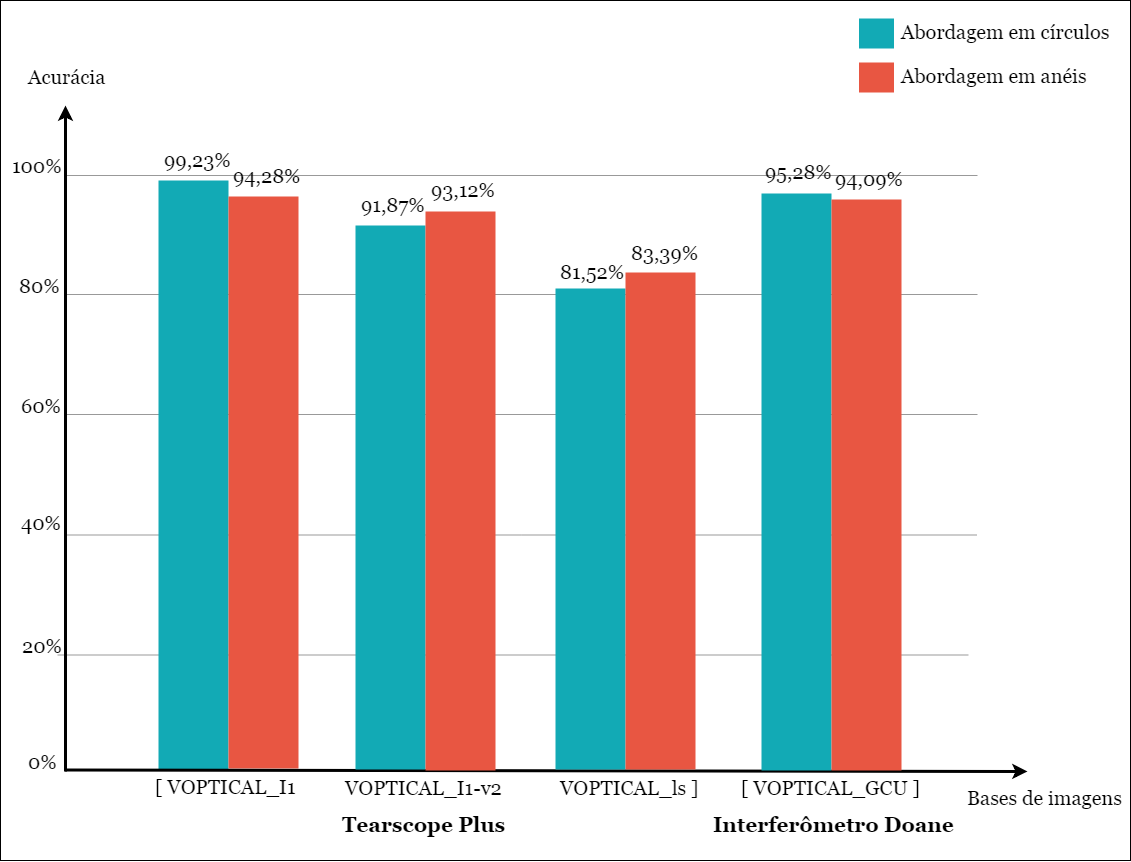
\includegraphics[width=0.8\textwidth]{figs/graficoKRipley1.png}
    \legend{Fonte: Elaborado pela autora.}
    \label{fig:graficoKRipley}
\end{figure}

A Figura~\ref{fig:graficoKRipley} ilustra o gráfico dos melhores resultados das abordagens em círculos e anéis da função K de \textit{Ripley} para todas as bases de imagens, empregada nesta dissertação. Nas bases de imagens capturadas com o Tearscope Plus os melhores resultados foram usando a abordagem em anéis, somente a base VOPTICAL\_I1 obteve melhor resultado utilizando a abordagem em círculos. Acredita-se que, as amostras adicionadas na versão atualizada (VOPTICAL\_I1-v2) apresentaram melhor comportamento com as características extraídas da abordagem em anéis, do que as amostras da primeira versão.

Por outro lado, a base de imagens VOPTICAL\_GCU capturada com o Interferômetro Doane, apresenta o melhor resultado usando a abordagem em círculos. Pressupõe-se que, para esse tipo de imagens as informações cumulativas sobre as regiões do objeto, fornecidas pelo uso de círculos são necessárias, pois as regiões centrais contém informações relevantes para a discriminação das imagens. Além disso, é importante enfatizar que ambas abordagens produziram bons resultados para os diferentes tipos de imagens utilizadas no método proposto. Dessa forma, conclui-se que as características extraídas da função K de \textit{Ripley} aplicadas sobre ambas abordagens, possuem um alto poder de discriminação dos padrões de interferência da camada lipídica do filme lacrimal.

%É importante enfatizar que um número maior de amostras aumenta a heterogeneidade e, consequentemente leva os experimentos a estarem sob circunstâncias mais realistas. Tendo em vista isto, é possível verificar que as bases de imagens VOPTICAL\_I1-v2 e VOPTICAL\_Is possuem um número maior de amostras e apresentam bons resultados, sendo bastante similares entre as abordagens. Portanto, conclui-se que as características extraídas da função K de \textit{Ripley} aplicadas sobre ambas abordagens, possuem um alto poder de discriminação dos padrões de interferência da camada lipídica do filme lacrimal.

\begin{figure}[!ht]
    \centering
    \caption{Gráfico dos principais resultados dos índices de diversidade filogenética para a base VOPTICAL\_GCU.}
    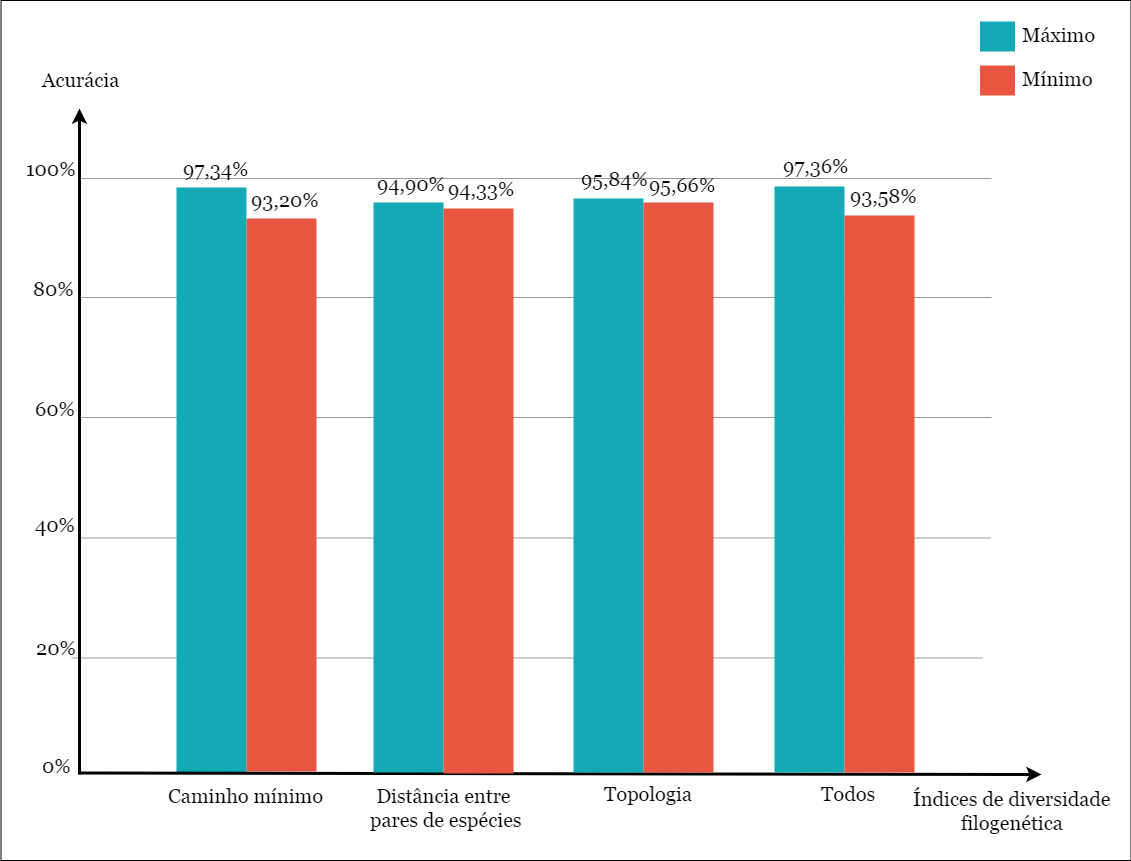
\includegraphics[width=0.8\textwidth]{figs/graficoIndices1.png}
    \legend{Fonte: Elaborado pela autora.}
    \label{fig:graficoIndicesDF}
\end{figure}

O gráfico da Figura~\ref{fig:graficoIndicesDF} apresenta o melhor e o pior resultado produzido por cada grupo dos índices de diversidade filogenética para a base de imagens VOPTICAL\_GCU capturada com o Interferômetro Doane. Ao analisar os resultados, verifica-se que o melhor desempenho foi obtido ao combinar todos os índices de diversidade filogenética. Em suma, acredita-se que a combinação de todos os índices de diversidade permite uma melhor discriminação porque os índices se complementam, isto é, um índice pode destacar uma propriedade que outro não consegue.

Em relação aos piores desempenhos, pode-se observar que a maioria foram obtidos usando o classificador SVM, conforme extraídos dos resultados apresentados na Subseção~\ref{subsectionVOPTICAL_GCU}. O SVM foi originalmente projetado para classificação binária \cite{hsu2002comparison}, e o problema proposto neste trabalho trata-se de uma abordagem multiclasse. Logo, presume-se que ao aumentar o número de classes o classificador diminui seu poder de discriminação, apresentando resultados inferiores. Entretanto, a média dos piores resultados é superior a 93\%, superando os trabalhos relacionados.

%Observando os piores desempenhos apresentados na Subseção~\ref{subsectionVOPTICAL_GCU}, pode-se analisar que a maioria dos resultados produzidos foram usando o classificador SVM. Os SVMs foram originalmente projetadas para classificação binária,  o problema abordado nesta dissertação trata-se da classificação de 5 categorias, aumenta a complexidade do classificador.

%Observando os resultados apresentados na Subseção~\ref{subsectionVOPTICAL_GCU}, pode-se analisar que geralmente os piores desempenhos são usando o classificador SVM. O problema abordado pelo método proposto, trata-se de classificação multi-classes

%as amostras adicionadas na versão 2 da base se comportaram melhor com as características retiradas do anéis do que as imagens da versão 1 da base

\begin{figure}[!ht]
    \centering
    \caption{Gráfico dos principais resultados da combinação dos índices de diversidade filogenética e a função K de \textit{Ripley} para a base VOPTICAL\_GCU.}
    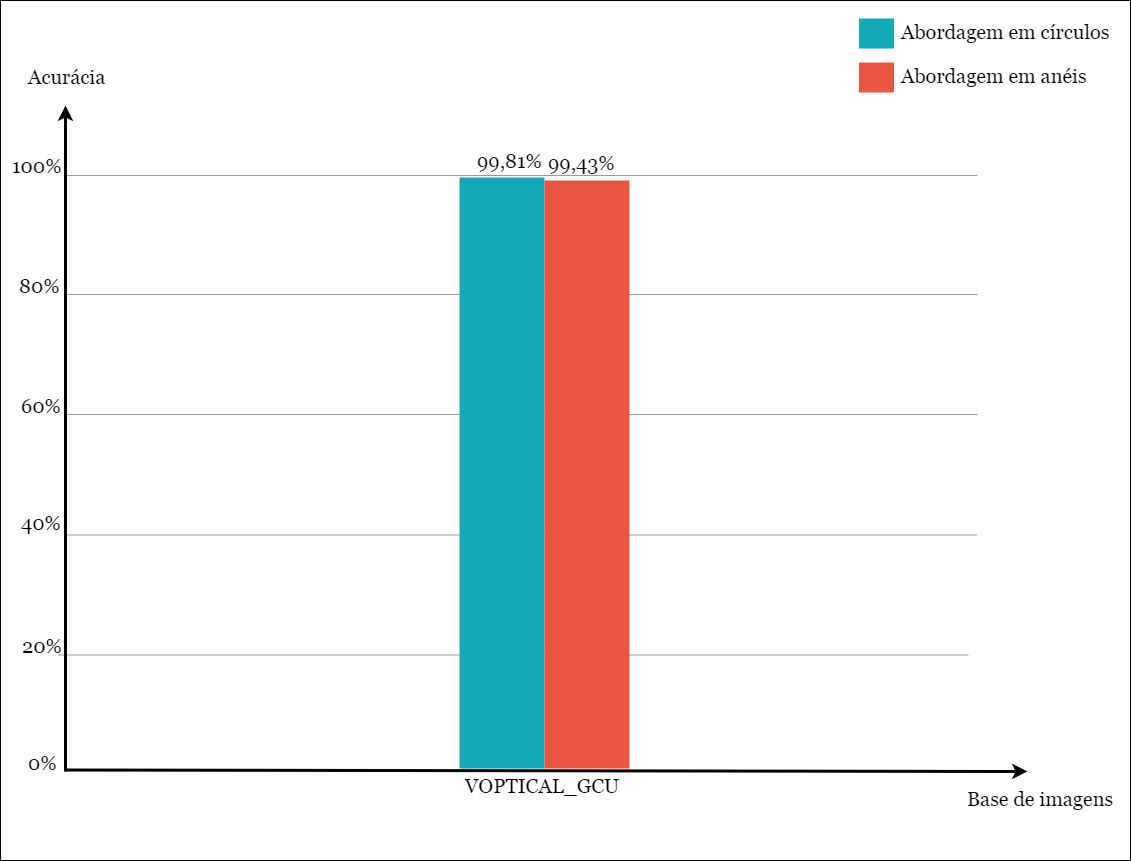
\includegraphics[width=0.8\textwidth]{figs/graficoKRipleyIndices.png}
    \legend{Fonte: Elaborado pela autora.}
    \label{fig:graficoIndicesDFKRipley}
\end{figure}

Finalizando, na Figura~\ref{fig:graficoIndicesDFKRipley} encontram-se os resultados da combinação dos índices de diversidade filogenética e a função K de \textit{Ripley} para a base de imagens capturada com o Interferômetro Doane (VOPTICAL\_GCU). Comparando os resultados produzidos para essa base de imagens, pode ser analisado que ao combinar os descritores, os resultados foram superiores aos produzidos usando somente a função K de \textit{Ripley} (Figura~\ref{fig:graficoKRipley}). Além disso, destaca-se que a abordagem em círculos produziu novamente o melhor resultado para a base VOPTICAL\_GCU, enfatizando que as informações cumulativas sobre as regiões do objeto, fornecidas pelo uso de círculos, são extremamente importantes para as imagens capturadas com o Interferômetro Doane. Entretanto, ambas abordagens apresentam bons resultados, concluindo que as características extraídas da função K de \textit{Ripley} e os índices de diversidade filogenética, possuem um alto poder de discriminação dos padrões de interferência da camada lipídica do filme lacrimal.

%Acreditamos, que o uso de anéis concêntricos elimina possíveis interferências de regiões centrais, fornecendo informações mais precisas a respeito das regiões periféricas da ROI..... Acreditamos que isso se deva às informações cumulativas sobre regiões periféricas do objeto, fornecidas pelo uso de círculos.

\section{Comparação do Método Proposto com os Trabalhos Relacionados}
\label{sec:comparacao}

Nesta seção é apresentada uma análise comparativa dos resultados obtidos pelo método proposto em relação aos trabalhos relacionados (Seção~\ref{sec:trabRelacionados}). A Tabela~\ref{tab:relacionados} apresenta um resumo desta comparação, fornecendo informações das técnicas, base de imagens, quantidade de imagens (amostra) e os valores médios de acurácia obtidos em cada trabalho.

Para realizar uma comparação mais rigorosa, os resultados obtidos em cada base do método proposto foi comparado com os trabalhos que utilizaram a mesma base de imagens, ou mesmo instrumento de captura das imagens. Entretanto, a comparação com outros trabalhos foi uma tarefa difícil, pois na literatura existem poucos trabalhos para quase todas as bases utilizadas no método proposto. Ainda assim, é possível elaborar alguns comentários em relação a esses trabalhos.

\definecolor{lightgray}{gray}{0.94}
\begin{table}[!ht]
\centering
\onehalfspacing
\caption{Comparação do método proposto com os trabalhos relacionados.}
\label{tab:relacionados}
\resizebox{\columnwidth}{!}{%
\begin{tabular}{lcp{8cm}cccc}
\cline{2-6} \parbox[t]{4mm}{\multirow{25}{*}{\rotatebox[origin=c]{90}{\textbf{Tearscope Plus}}}}
 & \textbf{Trabalho} & \centering \textbf{Técnica(s)} & \textbf{Base} & \textbf{Amostra} & \textbf{Acurácia} \\ \cline{2-6} 
 & (REMESEIRO et al., 2018) \cellcolor{lightgray} & Matriz de coocorrência no espaço de cor L*a*b* \cellcolor{lightgray} & VOPTICAL\_I1 \cellcolor{lightgray} & 105 \cellcolor{lightgray} & 96\% \cellcolor{lightgray}\\
 & (REMESEIRO et al., 2014) & Filtros \textit{Butterworth}, \textit{Gabor}, transformada discreta de \textit{Wavelet}, campos aleatórios de \textit{Markov} e coocorrência, seleção de características CFS, consistência e INTERACT & VOPTICAL\_I1 & 105 & 97,14\% \\
 & (MÉNDES et al., 2013) \cellcolor{lightgray} & Matriz de coocorrência, seleção de características CFS e método TOPSIS \cellcolor{lightgray} & VOPTICAL\_I1 \cellcolor{lightgray} & 105 \cellcolor{lightgray} & 95\% \cellcolor{lightgray}\\
 & (REMESEIRO et al., 2012) & Matriz de coocorrência em espaços de cores & VOPTICAL\_I1 & 105 & 96,19\% \\
 & (REMESEIRO et al., 2011) \cellcolor{lightgray} & Filtros \textit{Butterworth}, \textit{Gabor}, transformada discreta de \textit{Wavelet}, campos aleatórios de \textit{Markov} e coocorrência \cellcolor{lightgray} & VOPTICAL\_I1 \cellcolor{lightgray} & 105 \cellcolor{lightgray} & 96,19\% \cellcolor{lightgray}\\
 & (RAMOS et al., 2011) & Banco de filtros passa banda & VOPTICAL\_I1 & 105 & 91,43\% \\ \cline{2-6} 
 & (REMESEIRO et al., 2016) \cellcolor{lightgray} & Matriz de coocorrência, seleção de características CFS \cellcolor{lightgray} & VOPTICAL\_I1-v2 \cellcolor{lightgray} & 128 \cellcolor{lightgray} & 96,09\% \cellcolor{lightgray} \\ \cline{2-6} 
 & (REMESEIRO et al., 2014) & Filtros \textit{Butterworth}, \textit{Gabor}, transformada discreta de \textit{Wavelet}, campos aleatórios de \textit{Markov} e coocorrência, seleção de características CFS, consistência e INTERACT & VOPTICAL\_Is & 406 & 93,84\% \\ \cline{2-6} 
 & (CALVO et al., 2010) \cellcolor{lightgray} & Banco rotacionalmente invariante de filtros passa banda \cellcolor{lightgray} & PRIVADA \cellcolor{lightgray} & 91 \cellcolor{lightgray} & 86,41\% \cellcolor{lightgray}\\ \cline{2-6} \parbox[t]{5mm}{\multirow{4}{*}{\rotatebox[origin=c]{90}{\textbf{Int. Doane}}}}
 & (REMESEIRO et al., 2015) & Processamento de sinais, modelo e estatístico & VOPTICAL\_GCU & 106 & 93,40\% \\
 & (VILLAVERDE et al., 2014) \cellcolor{lightgray} & Processamento de sinais, modelo e estatístico e seleção de características CFS, consistência e INTERACT \cellcolor{lightgray} & VOPTICAL\_GCU \cellcolor{lightgray} & 106 \cellcolor{lightgray} & 91,51\% \cellcolor{lightgray}\\ \cline{2-6}
 & Método Proposto & Função K de \textit{Ripley} & \begin{tabular}[c]{@{}c@{}}VOPTICAL\_I1\\ VOPTICAL\_I1-v2\\ VOPTICAL\_ls\\ VOPTICAL\_GCU\end{tabular} & \begin{tabular}[c]{@{}c@{}}105\\ 128\\ 406\\ 106\end{tabular} & \begin{tabular}[c]{@{}c@{}}99,23\%\\ 93,12\%\\ 83,39\%\\ 95,28\%\end{tabular} \\ \cline{3-6} 
 &  & Índices de Diversidade Filogenética & VOPTICAL\_GCU & 106 & 97,36\% \\ \cline{3-6} 
 &  & Função K de \textit{Ripley} e Índices de Div. Filog. & VOPTICAL\_GCU & 106 & 99,81\% \\ \cline{2-6} 
\end{tabular}
}
\end{table}

\begin{comment}
\begin{table}[!ht]
\centering
\onehalfspacing
\caption{Comparação do método proposto com os trabalhos relacionados.}
\label{tab:relacionados}
\resizebox{\columnwidth}{!}{%
\begin{tabular}{cp{8cm}cccc}
\hline \hline
\textbf{Trabalho} & \textbf{Técnica(s)} & \textbf{Base} & \textbf{Amostra} & \textbf{Acurácia} \\ \hline \hline
\rowcolor{lightgray} (REMESEIRO et al., 2014) & Filtros \textit{Butterworth}, \textit{Gabor}, transformada discreta de \textit{Wavelet}, campos aleatórios de \textit{Markov} e coocorrência, seleção de características CFS, consistência e INTERACT & VOPTICAL\_I1 & 105 & 97,14\% \\
\rowcolor{lightgray} (REMESEIRO et al., 2012) & Matriz de coocorrência em espaços de cores & VOPTICAL\_I1 & 105 & 96,19\% \\
\rowcolor{lightgray} (REMESEIRO et al., 2011) & Filtros \textit{Butterworth}, \textit{Gabor}, transformada discreta de \textit{Wavelet}, campos aleatórios de \textit{Markov} e coocorrência & VOPTICAL\_I1 & 105 & 96,19\% \\
\rowcolor{lightgray} (REMESEIRO et al., 2018) & Matriz de coocorrência no espaço de cor L*a*b* & VOPTICAL\_I1 & 105 & 96\% \\
\rowcolor{lightgray} (MÉNDES et al., 2013) & Matriz de coocorrência, seleção de características CFS e método TOPSIS & VOPTICAL\_I1 & 105 & 95\% \\
\rowcolor{lightgray} (RAMOS et al., 2011) & Banco de filtros passa banda & VOPTICAL\_I1 & 105 & 91,43\% \\ \hline
(REMESEIRO et al., 2016) & Matriz de coocorrência, seleção de características CFS & VOPTICAL\_I1-v2 & 128 & 96,09\% \\ \hline
\rowcolor{lightgray} (REMESEIRO et al., 2014) & Filtros \textit{Butterworth}, \textit{Gabor}, transformada discreta de \textit{Wavelet}, campos aleatórios de \textit{Markov} e coocorrência, seleção de características CFS, consistência e INTERACT & VOPTICAL\_Is & 406 & 93,84\% \\ \hline
(CALVO et al., 2010) & Banco rotacionalmente invariante de filtros passa banda & PRIVADA & 91 & 86,41\% \\ \hline
\rowcolor{lightgray}(REMESEIRO et al., 2015) & Processamento de sinais, modelo e estatístico & VOPTICAL\_GCU & 106 & 93,40\% \\
\rowcolor{lightgray} (VILLAVERDE et al., 2014) & Processamento de sinais, modelo e estatístico e seleção de características CFS, consistência e INTERACT & VOPTICAL\_GCU & 106 & 91,51\% \\ \hline
Método Proposto & Função K de \textit{Ripley} & \begin{tabular}[c]{@{}c@{}}VOPTICAL\_I1\\ VOPTICAL\_I1-v2\\ VOPTICAL\_Is\\ VOPTICAL\_GCU\end{tabular} & \begin{tabular}[c]{@{}c@{}}105\\ 128\\ 406\\ 106\end{tabular} & \begin{tabular}[c]{@{}c@{}}99,23\%\\ 93,12\%\\ 83,39\%\\ 95,28\%\end{tabular} \\ \cline{2-5} 
 & Índices de Diversidade Filogenética & VOPTICAL\_GCU & 106 & 97,36\% \\ \cline{2-5} 
 & Função K de \textit{Ripley} e Índices de Div. Filog. & VOPTICAL\_GCU & 106 & 99,81\% \\ \hline
\end{tabular}
}
\end{table}
\end{comment}

No trabalho de \citeonline{calvo2010color} a base privada utilizada é composta por imagens capturadas com o Teascope Plus, portanto é possível realizar comparação com as bases de imagens VOPTICAL\_I1, VOPTICAL\_I1-v2 e VOPTICAL\_Is utilizadas no método proposto, pois são capturadas com o mesmo instrumento. Em relação aos trabalhos que usaram a base de imagens VOPTICAL\_I1, é possível observar que a performance do método proposto que usa a mesma base foi superior a todos os trabalhos, em termos de acurácia.

%Os trabalhos que usaram as bases de imagens VOPTICAL\_I1-v2 e VOPTICAL\_Is, obtiveram taxas de acerto maiores que as do método proposto. Entretanto, a quantidade de amostras das bases VOPTICAL\_I1-v2 e VOPTICAL\_Is usadas no método proposto, são expressivamente maiores do que as utilizadas no trabalho de \citeonline{calvo2010color}, sendo 28,91\% e 77,59\% superiores. Um número maior de amostras aumenta a heterogeneidade e, consequentemente leva os experimentos a estarem sob circunstâncias mais realistas.

Os trabalhos que usaram as bases de imagens VOPTICAL\_I1-v2 e VOPTICAL\_Is obtiveram taxas de acerto maiores que as do método proposto, porém próximos. Em relação a base privada, é possível observar que o resultado alcançado é inferior aos resultados produzidos pelo método proposto, e a quantidade de amostras das bases VOPTICAL\_I1-v2 e VOPTICAL\_Is são expressivamente maiores do que as utilizadas na base privada, sendo superior 28,91\% e 77,59\%, respectivamente. É importante destacar que um número maior de amostras aumenta a heterogeneidade e, consequentemente leva os experimentos a estarem sob circunstâncias mais realistas.

Os trabalhos de \citeonline{remeseiro2015automatic} e \citeonline{villaverde2014feature} realizam testes na base de imagens VOPTICAL\_GCU. Observando os resultados desses trabalhos e comparando com os resultados alcançados no método proposto quando usa a base VOPTICAL\_GCU, é possível verificar que o método proposto apresenta resultados superiores aos dois trabalhos, tanto ao aplicar somente o descritor da função K de \textit{Ripley} ou os índices de diversidade filogenética, quanto concatenando ambos descritores. 

Finalmente, é importante destacar que neste trabalho é realizada uma análise detalhada dos resultados, por meio das médias obtidas na acurácia, desvio padrão, área sob a curva ROC, \textit{Kappa} e \textit{F-Measure}, isto é, não são considerados apenas resultados isolados. Dessa forma, é possível verificar a consistência dos resultados produzidos para discriminação dos padrões.

Vale ressaltar que o objetivo deste trabalho não é superar todas as metodologias descritas na literatura, mas contribuir com o desenvolvimento de um novo método automático para classificar os padrões de interferência da camada lipídica em imagens do filme lacrimal.

\section{Considerações Finais}

Neste capítulo foram apresentados e discutidos os resultados obtidos pelos experimentos realizados no desenvolvimento do método proposto. Também foi feito um comparativo com os trabalhos relacionados, como forma de analisar a relevância da pesquisa desenvolvida.

No geral, os resultados obtidos podem ser considerados promissores, sendo
comparáveis aos melhores trabalhos descritos na literatura. As maiores taxas de acerto
foram obtidas com a utilização do algoritmo \textit{Greedy Stepwise} para seleção das características mais relevantes da junção dos descritores da função K de \textit{Ripley} e índices de diversidade filogenética, onde foi possível alcançar valores médios de acurácia superiores a 99\%.

No próximo capítulo são apresentadas as conclusões a cerca da pesquisa desenvolvida nesta dissertação. Também serão apontadas algumas de suas limitações, bem como apresentadas sugestões para trabalhos futuros.
% estudo de caso 1: RA; estudo de caso 2: RV;
\chapter{Conclusão}
\phantom{2}

A diferenciação dos padrões de interferência da camada lipídica, em imagens do filme lacrimal exclusivamente pela análise de textura é uma tarefa difícil, principalmente devido ao fato de ser muito comum as categorias da camada lipídica possuírem características de textura semelhantes. Neste contexto, técnicas que auxiliem o desenvolvimento de sistemas CAD e CADx são de grande contribuição para o meio científico.

Nesta dissertação foi apresentado um método de classificação das categorias da camada lipídica em imagens do filme lacrimal para auxiliar no diagnóstico da Síndrome do Olho Seco. O objetivo deste trabalho foi apresentar a viabilidade da utilização dos descritores de textura baseados na geostatística e biologia para a discriminação dos padrões de interferência da camada lipídica do filme lacrimal.

O método proposto foi validado através de experimentos usando as bases de imagens capturadas com o Tearscope Plus: VOPTICAL\_I1, VOPTICAL\_I2-v2 e VOPTICAL\_Is; e capturadas com o Interfêrometro Doane: VOPTICAL\_GCU. Em resumo, os descritores merecem destaque no método proposto, considerados também como as principais contribuições desta dissertação. A primeira é a adaptação e o uso dos conceitos da biologia, mais precisamente dos índices de diversidade filogenética e das árvores filogenéticas; A segunda foi a combinação da abordagem estrutural por meio da técnica LBP e a abordagem geostatística através das técnicas da função K de \textit{Ripley}.

Após a etapa de extração de características, o conjunto gerado foi submetido a uma série de experimentos de classificação na etapa de reconhecimento de padrões, no qual foram utilizados os classificadores SVM, RF, NB e BN. Usando apenas o descritor K de \textit{Ripley}, os melhores resultados alcançados para as bases de imagens VOPTICAL\_I1, VOPTICAL\_I1-v2, VOPTICAL\_Is e VOPTICAL\_GCU foram obtidos ao utilizar o algoritmo \textit{Greedy Stepwise} para seleção automática das características mais relevantes, onde foram alcançados média de acurácia de 99,23\%, 93,12\%, 83,39\% e 95,28\% para as respectivas bases de imagens.

O melhor resultado dos experimentos usando o descritor dos índices de diversidade filogenética para a base de imagens VOPTICAL\_GCU foi aplicando todos os índices de diversidade filogenética, onde alcançou uma média de acurácia de 97,36\%. Por fim, a combinação de todos os índices de diversidade filogenética, a função K de \textit{Ripley} e a seleção de características, apresentou o melhor resultado para a base em questão, resultando em uma média de acurácia de 99,81\%.

Os resultados alcançados nesta dissertação são considerados promissores, sendo comparáveis aos melhores trabalhos descritos na literatura. A partir dos valores obtidos foi possível demonstrar que a utilização dos descritores de textura é bastante viável para caracterização dos padrões de interferência da camada lipídica do filme lacrimal e, portanto, poderão ser utilizados em metodologias CADx para auxílio do diagnóstico da Síndrome do Olho Seco.

Apesar de ter obtido bons resultados no geral, o método proposto possui alguns experimentos que podem ser realizados para melhorar alguns resultados, entre os quais citam-se: a realização de experimentos com os descritores dos índices de diversidade filogenética para as imagens das bases capturadas com o Tearscope Plus, pois nesta pesquisa não foi possível a realização do mesmo, devido ao tempo de conclusão do mestrado.

Conforme apresentado nos trabalhos relacionados, existe um grande interesse da comunidade científica em pesquisas na área médica, devido a relevância deste tema. Desta forma, espera-se que os frutos desta pesquisa possam ser utilizados no futuro em novas metodologias, de modo que sejam sanadas algumas de suas limitações. Assim, como sugestão para trabalhos futuros estão:

\begin{enumerate}
    \item Realizar experimentos com os índices de diversidade filogenética nas imagens das bases capturadas com o Tearscope Plus;
    
    \item Investigar a aplicabilidade de novos índices de diversidade, como os índices funcionais, que possuem como objetivo analisar as relações entre as espécies e possíveis características, como evolução;
    
    \item Usar variações do LBP para geração dos padrões como os algoritmos de LBP circular e de
    \textit{Completed Local Binary Pattern} (CLBP), visto que estas abordagens analisam um número maior de vizinhos no cálculo do LBP, por serem circulares;
    
    \item Avaliar outras técnicas de estatística espacial como, índice de \textit{Moran}, de \textit{Getis} e Coeficiente de \textit{Geary};
    
    \item Analisar a textura da ROI em outras sub-regiões, como máscaras internas e externas, horizontal, vertical, janelas e também, em outros espaços de cores;
    
    \item Utilizar outro método de seleção de características para redução da dimensionalidade de características usando a função K de \textit{Ripley};
    
    \item Realizar testes com outras técnicas de aprendizado de máquina, como abordagens de aprendizagem profunda, ou outros classificadores como \textit{Random Tree}, \textit{Multilayer Perceptron} e \textit{AdaBoost};
    
    \item Aplicar o método proposto para a caracterização de textura de anormalidades de outros tipos de imagens como, por exemplo, de mama; e
    
    \item Empregar o método proposto para outros tipos de imagens, tais como imagens de tomografia de coerência óptica.
    
\end{enumerate}

\section{Produções Científicas}

A \autoref{tab:artigos} apresenta a lista de artigos científicos publicados e submetidos que possuem relação com o método proposto neste trabalho.

\definecolor{lightgray}{gray}{0.94}
\begin{table}[!ht]
\centering
%\onehalfspacing
\rowcolors{1}{}{lightgray}
\caption{Artigos submetidos e publicados do mestrado. Legenda: Publicado (PU) e submetido (SU).}
\label{tab:artigos}
\begin{tabular}{cp{10cm}ccc}
\hline
\textbf{Local} & \centering \textbf{Artigo} & \textbf{Qualis} & \textbf{Status} \\ \hline \hline
Simpósio & \textbf{CRUZ, L. B.}; ARAÚJO, J. D.; SOUSA, J. A.; ALMEIDA, J. D.; JÚNIOR, G. B.; SILVA, A. C.; PAIVA, A. C. Classificação do Filme Lacrimal usando a Função K de Ripley como Descritor de Textura. Simpósio Brasileiro de Computação Aplicada à Saúde (SBCAS\_CSBC), v. 18, n. 1/2018, 2018. & B4 & PU \\
Simpósio & \textbf{CRUZ, L. B.}; ARAÚJO, J. D. L.; SOUZA, J. C.; SOUSA, J. A.; ALMEIDA, J. D. S.; JUNIOR, G. B.; SILVA, A. C.; PAIVA, A. C. Tear Film Classification Using Phylogenetic Diversity Indexes as Texture Descriptor. In: 2018 IEEE Symposium on Computers and Communications (ISCC). IEEE, 2018. p. 00853-00858. & A2 & PU \\
Periódico & \textbf{CRUZ, L. B.}; SOUZA, J. C.; SOUSA, J. A.; SANTOS, A. M.; PAIVA, A. C.; ALMEIDA, J. D. S.; SILVA, A. C.; JÚNIOR, G. B. Dry Eye Classification in Interferometry Images using Phylogenetic Diversity Indexes. Journal of Visual Communication and Image Representation. & A2 & SU \\ \hline
\end{tabular}
\end{table}


% \include{proposta de marcador_natural}
% related works - proposta - resultados
% \include{cap4_estimacao_pose}
% related works - proposta - resultados
% \include{cap5_panoramas_aumentados}
% related works - proposta - resultados
% \chapter{Conclusão}
\phantom{2}

A diferenciação dos padrões de interferência da camada lipídica, em imagens do filme lacrimal exclusivamente pela análise de textura é uma tarefa difícil, principalmente devido ao fato de ser muito comum as categorias da camada lipídica possuírem características de textura semelhantes. Neste contexto, técnicas que auxiliem o desenvolvimento de sistemas CAD e CADx são de grande contribuição para o meio científico.

Nesta dissertação foi apresentado um método de classificação das categorias da camada lipídica em imagens do filme lacrimal para auxiliar no diagnóstico da Síndrome do Olho Seco. O objetivo deste trabalho foi apresentar a viabilidade da utilização dos descritores de textura baseados na geostatística e biologia para a discriminação dos padrões de interferência da camada lipídica do filme lacrimal.

O método proposto foi validado através de experimentos usando as bases de imagens capturadas com o Tearscope Plus: VOPTICAL\_I1, VOPTICAL\_I2-v2 e VOPTICAL\_Is; e capturadas com o Interfêrometro Doane: VOPTICAL\_GCU. Em resumo, os descritores merecem destaque no método proposto, considerados também como as principais contribuições desta dissertação. A primeira é a adaptação e o uso dos conceitos da biologia, mais precisamente dos índices de diversidade filogenética e das árvores filogenéticas; A segunda foi a combinação da abordagem estrutural por meio da técnica LBP e a abordagem geostatística através das técnicas da função K de \textit{Ripley}.

Após a etapa de extração de características, o conjunto gerado foi submetido a uma série de experimentos de classificação na etapa de reconhecimento de padrões, no qual foram utilizados os classificadores SVM, RF, NB e BN. Usando apenas o descritor K de \textit{Ripley}, os melhores resultados alcançados para as bases de imagens VOPTICAL\_I1, VOPTICAL\_I1-v2, VOPTICAL\_Is e VOPTICAL\_GCU foram obtidos ao utilizar o algoritmo \textit{Greedy Stepwise} para seleção automática das características mais relevantes, onde foram alcançados média de acurácia de 99,23\%, 93,12\%, 83,39\% e 95,28\% para as respectivas bases de imagens.

O melhor resultado dos experimentos usando o descritor dos índices de diversidade filogenética para a base de imagens VOPTICAL\_GCU foi aplicando todos os índices de diversidade filogenética, onde alcançou uma média de acurácia de 97,36\%. Por fim, a combinação de todos os índices de diversidade filogenética, a função K de \textit{Ripley} e a seleção de características, apresentou o melhor resultado para a base em questão, resultando em uma média de acurácia de 99,81\%.

Os resultados alcançados nesta dissertação são considerados promissores, sendo comparáveis aos melhores trabalhos descritos na literatura. A partir dos valores obtidos foi possível demonstrar que a utilização dos descritores de textura é bastante viável para caracterização dos padrões de interferência da camada lipídica do filme lacrimal e, portanto, poderão ser utilizados em metodologias CADx para auxílio do diagnóstico da Síndrome do Olho Seco.

Apesar de ter obtido bons resultados no geral, o método proposto possui alguns experimentos que podem ser realizados para melhorar alguns resultados, entre os quais citam-se: a realização de experimentos com os descritores dos índices de diversidade filogenética para as imagens das bases capturadas com o Tearscope Plus, pois nesta pesquisa não foi possível a realização do mesmo, devido ao tempo de conclusão do mestrado.

Conforme apresentado nos trabalhos relacionados, existe um grande interesse da comunidade científica em pesquisas na área médica, devido a relevância deste tema. Desta forma, espera-se que os frutos desta pesquisa possam ser utilizados no futuro em novas metodologias, de modo que sejam sanadas algumas de suas limitações. Assim, como sugestão para trabalhos futuros estão:

\begin{enumerate}
    \item Realizar experimentos com os índices de diversidade filogenética nas imagens das bases capturadas com o Tearscope Plus;
    
    \item Investigar a aplicabilidade de novos índices de diversidade, como os índices funcionais, que possuem como objetivo analisar as relações entre as espécies e possíveis características, como evolução;
    
    \item Usar variações do LBP para geração dos padrões como os algoritmos de LBP circular e de
    \textit{Completed Local Binary Pattern} (CLBP), visto que estas abordagens analisam um número maior de vizinhos no cálculo do LBP, por serem circulares;
    
    \item Avaliar outras técnicas de estatística espacial como, índice de \textit{Moran}, de \textit{Getis} e Coeficiente de \textit{Geary};
    
    \item Analisar a textura da ROI em outras sub-regiões, como máscaras internas e externas, horizontal, vertical, janelas e também, em outros espaços de cores;
    
    \item Utilizar outro método de seleção de características para redução da dimensionalidade de características usando a função K de \textit{Ripley};
    
    \item Realizar testes com outras técnicas de aprendizado de máquina, como abordagens de aprendizagem profunda, ou outros classificadores como \textit{Random Tree}, \textit{Multilayer Perceptron} e \textit{AdaBoost};
    
    \item Aplicar o método proposto para a caracterização de textura de anormalidades de outros tipos de imagens como, por exemplo, de mama; e
    
    \item Empregar o método proposto para outros tipos de imagens, tais como imagens de tomografia de coerência óptica.
    
\end{enumerate}

\section{Produções Científicas}

A \autoref{tab:artigos} apresenta a lista de artigos científicos publicados e submetidos que possuem relação com o método proposto neste trabalho.

\definecolor{lightgray}{gray}{0.94}
\begin{table}[!ht]
\centering
%\onehalfspacing
\rowcolors{1}{}{lightgray}
\caption{Artigos submetidos e publicados do mestrado. Legenda: Publicado (PU) e submetido (SU).}
\label{tab:artigos}
\begin{tabular}{cp{10cm}ccc}
\hline
\textbf{Local} & \centering \textbf{Artigo} & \textbf{Qualis} & \textbf{Status} \\ \hline \hline
Simpósio & \textbf{CRUZ, L. B.}; ARAÚJO, J. D.; SOUSA, J. A.; ALMEIDA, J. D.; JÚNIOR, G. B.; SILVA, A. C.; PAIVA, A. C. Classificação do Filme Lacrimal usando a Função K de Ripley como Descritor de Textura. Simpósio Brasileiro de Computação Aplicada à Saúde (SBCAS\_CSBC), v. 18, n. 1/2018, 2018. & B4 & PU \\
Simpósio & \textbf{CRUZ, L. B.}; ARAÚJO, J. D. L.; SOUZA, J. C.; SOUSA, J. A.; ALMEIDA, J. D. S.; JUNIOR, G. B.; SILVA, A. C.; PAIVA, A. C. Tear Film Classification Using Phylogenetic Diversity Indexes as Texture Descriptor. In: 2018 IEEE Symposium on Computers and Communications (ISCC). IEEE, 2018. p. 00853-00858. & A2 & PU \\
Periódico & \textbf{CRUZ, L. B.}; SOUZA, J. C.; SOUSA, J. A.; SANTOS, A. M.; PAIVA, A. C.; ALMEIDA, J. D. S.; SILVA, A. C.; JÚNIOR, G. B. Dry Eye Classification in Interferometry Images using Phylogenetic Diversity Indexes. Journal of Visual Communication and Image Representation. & A2 & SU \\ \hline
\end{tabular}
\end{table}


\renewcommand{\nomname}{\listadesiglasname\bigskip}
\postextual
  

\bibliography{capitulos/referencias}


%\begin{apendicesenv}

% Imprime uma página indicando o início dos apêndices
%\partapendices

%\begin{KeepFromToc} nao necessario

%\chapter*{APÊNDICE A - Termo de Consentimento Livre e Esclarecido}
%\begin{figure}[!ht]
%\centering
%\includegraphics[scale=0.80]{termo.pdf}
%\end{figure}

%auto_depo

%\chapter*{APÊNDICE B - Termo de Autorização de Depoimento}
%\begin{figure}[!ht]
%\centering
%\includegraphics[scale=0.80]{auto_depo.pdf}
%\end{figure}

%\chapter*{APÊNDICE C - Roteiro de Entrevista}
%\begin{figure}[!ht]
%\centering
%\includegraphics[scale=0.80]{roteiro.pdf}
%\end{figure}

%\end{KeepFromToc} nao necessario

%\end{apendicesenv}

%\begin{anexosenv}

% Imprime uma página indicando o início dos anexos
%\partanexos

%\chapter*{ANEXO A - RESOLUÇÃO Nº 64, DE 05 DE DEZEMBRO DE 2014}
%\begin{figure}[!ht]
%\centering
%\includegraphics[scale=0.80]{res64.pdf}
%\end{figure}

%\includepdf[pages={2-},scale=0.9,pagecommand={}]{res64.pdf}
% \end{anexosenv}

\end{document}
